\documentclass[a4paper]{cas-sc}
\usepackage{soul}

%%%%%%%%%%%%%
% \usepackage[numbers]{natbib}
\usepackage[authoryear]{natbib}
% \usepackage[authoryear,longnamesfirst]{natbib}

% Author macros
\def\tsc#1{\csdef{#1}{\textsc{\lowercase{#1}}\xspace}}
\tsc{WGM}
\tsc{QE}

\usepackage{amssymb}
\usepackage{amsmath,amsfonts}
\usepackage{caption}
\captionsetup[figure]{name={Fig.},labelsep=period,singlelinecheck=off}
% \usepackage{algorithmic}
\usepackage[linesnumbered,ruled]{algorithm2e}
\usepackage{array}
% \usepackage[caption=false,font=normalsize,labelfont=sf,textfont=sf]{subfig}
\usepackage{textcomp}
\usepackage{stfloats}
\usepackage{url}
\usepackage{verbatim}
\usepackage{graphicx}
\usepackage{epstopdf}
\epstopdfsetup{outdir=build/}
% \usepackage{subcaption}
%\usepackage{cite}
%\usepackage{biblatex}  
\usepackage{natbib}
%\usepackage[options]{natbib}
%\addbibresource{ref.bib}
% \hyphenation{op-tical net-works semi-conduc-tor IEEE-Xplore}
% updated with editorial comments 8/9/2021
%\usepackage{hyperref}
\usepackage{subfigure} %By myself
\usepackage{amssymb}
\usepackage{multirow}
\usepackage{mathrsfs}
%\usepackage{mathptmx}
\usepackage{amsthm}
\newtheorem{myDef}{Definition}
\newtheorem{myTheo}{Theorem}
\newtheorem{mypro}{Proposition}
\newtheorem{myex}{Example}
%\usepackage{booktabs}
% \usepackage{algorithmic}
\usepackage{array}
\usepackage{booktabs}
\usepackage{array, caption, threeparttable}
\usepackage[font=small,labelfont=bf]{caption}
\captionsetup[table]{
  labelsep=newline,
  singlelinecheck=false,
}
\usepackage{xcolor} % 提供颜色和高亮功能的宏包
\usepackage{soul}  % 提供\hl命令用于文本高亮
\usepackage{algpseudocode} 
\usepackage{threeparttable}
\usepackage{hyperref}
\hypersetup{%hypertex=true,
            colorlinks=true,
            linkcolor=blue,
            anchorcolor=blue,
            citecolor=blue}
\usepackage{algpseudocode}
\renewcommand{\algorithmicrequire}{\textbf{Input:}}  % Use Input in the format of Algorithm
\renewcommand{\algorithmicensure}{\textbf{Output:}} % Use Output in the format of Algorithm
\newtheorem{remark}{Remark}   
\renewcommand{\qedsymbol}{}
%reference
\usepackage{hyperref}
\usepackage{threeparttable}
% \usepackage{apacite}  % 导入apacite宏包
% \bibliographystyle{apacite}  % 设置参考文献样式
\usepackage{xcolor}
\usepackage{float}
\restylefloat{figure}
\begin{document}

\let\WriteBookmarks\relax
\def\floatpagepagefraction{1}
\def\textpagefraction{.001}



%------------------------ Title ------------------------

\title [mode = title]{Dual Balanced Large Marginal Machine for Imbalanced Data Classification}

\shorttitle{Dual Balanced Large Marginal Machine for Imbalanced Data Classification}

%------------------------ Authors ------------------------
% short author
\shortauthors{Gu et~al.}

%% ---- First Author ----
\author[1]{Pingping Gu}
\credit{Writing - original draft, Methodology, Software, Writing - review editing}
\affiliation[1]{
    organization={School of Transportation and Civil Engineering, Nantong University},
    city={Nantong},
    citysep={},
    postcode={400715}, 
    country={China}}
\affiliation[2]{
    organization={College of Artificial Intelligence, Southwest University},
    city={Chongqing},
    citysep={},
    postcode={400715}, 
    country={China}}

%% ---- Second Author ----
\author[2]{Denghao Dong}
\credit{Software, Formal analysis}


%% ---- Third Author ----
\author[1]{Quan Shi}
\credit{Writing – review $\&$ editing}

%% ---- Four Author ----
\author[2]{Fudi Wang}
\credit{Software – review $\&$ editing}

%% ---- Fi Author ----
\author[2]{Guojun Huang}[orcid=0000-0002-4519-7068]
\credit{Validation, Writing - review editing, Funding acquisition}
\cormark[1]
\cortext[cor1]{Corresponding author: Guojun Huang \\
\qquad \qquad E-mail address: pingpinggu0513@163.com (P. Gu), \\ dhdong1129@163.com (D. Dong), sq@ntu.edu.cn (Q. Shi),\\blue16@email.swu.edu.cn (F. Wang), aikyoko@163.com (G. Huang)}


\begin{abstract}
As a modification of Support Vector Machine (SVM), Large Margin Distribution Machine (LDM) enhances generalization performance by integrating the marginal distribution of samples into the objective function. Nevertheless, the current LDM models (LDMs) still suffer from limitations in imbalanced classification tasks, i.e., the classification hyperplane tends to be skewed towards the minority class. Moreover, the inherited hinge loss function from SVM results in inferior noise immunity and stability. To overcome these limitations, we propose a novel dual balanced (DB) distance function to replace the traditional distance metric and introduce the unified pinball loss (UP) as a replacement for the inherited hinge loss, which significantly enhances the model's generalization capacity in imbalanced classification tasks. Specifically, we combine the imbalance level and bias to construct a pair of composite distances for the majority and minority classes, respectively. The dual balanced distance contributes to reducing the slackness of the minority class and the influence of the majority class, leading to a balanced classification hyperplane. Additionally, the introduction of the unified pinball loss function improves the model's robustness and noise resistance. We have evaluated our proposed model in the fields of meteorology, finance, healthcare, and engineering, demonstrating its superior performance.


\end{abstract}
% Compared with Support Vector Machine (SVM), Large Margin Distribution Machine (LDM) has better generalization performance by adding the marginal distribution of the sample point. However, LDM still suffers from noise and boundary sample points because it inherits the hinge loss function from SVM, which is related to the shortest distance between sample sets and the corresponding classifier. In contrast, the Unified Pinball (UP) loss function is related to quantile distance, and is less affected by noise. Therefore, this paper introduces the UP loss into LDM, and proposes a novel Large Margin Distribution Machine Classifier with Cost-Sensitive Unified Pinball Loss (DBUPLDM) that achieves better anti-noise performance. When constructing the model, the hinge loss in the objective function is replaced by the UP loss, and each sample point is assigned with a penalty term, which weakens the problems of noise sensitivity and data imbalance. Furthermore, to handle more general problems, we expand DBUPLDM to multi-class (DBUPMLDM) by leveraging the one-vs-one strategy. Finally, to testify the effectiveness of the proposed models, we conduct a series of experiments on the artificial datasets, UCI datasets and UCI datasets with artificial noise. The experimental results show that the proposed models have excellent noise immunity, stability and classification accuracy.

\begin{keywords}
Imbalanced Data \sep Large Marginal Distribution Machine \sep Composite Distance \sep Pinball Loss.
\end{keywords}

\maketitle

\section{Introduction}
Support Vector Machine (SVM) is a widely used machine learning classification method introduced by \cite{cortes1995support}. {\color{blue} It has been widely utilized in classification \citep{rezvani2021class,chen2025ams,naveen2025effnet,rezvani2022intuitionistic,YU2023105751}, face detection \citep{tiwari2024comprehensive,rashad2024ccnn}, and other fields \citep{huang2021railway,yang2022novel,POURHOSSEINI2023106780,LYAQINI2024107567}.} To minimize the structural risk, SVM maximizes the minimum interval between two classes, i.e., maximizes the distance between the support vector and the classification hyperplane. However, according to the marginal theory, marginal distribution, rather than the minimum interval, is more important for the generalization performance \citep{reyzin2006boosting}. Such a conjecture has been theoretically investigated \citep{wang2011refined,gao2013doubt}, and the assertion is finally proved by \cite{gao2013doubt}. Therefore, based on this theory, Zhang et al. proposed the Large Margin Distribution Machine (LDM), which achieves better generalization performance \citep{zhang2014large}. LDM considers the overall distribution of samples, not just support vectors \citep{huang2016solution,zhang2023novel}. Specifically, it introduces two statistics, margin mean and margin variance, into the objective function, and optimizes the interval distribution while ensuring the minimum structural risk. 

However, the introduction of the second-order statistic in LDM also poses some problems. Since the LDM needs to maximize the mean margin, it leads to a hyperplane skewed toward the minority classes, which generates low generalization performance for the samples of fewer classes. Therefore, the classification task for imbalanced datasets becomes less accurate and performance degrades. Moreover, since LDM is an improvement on the SVM, it is a direct addition of two statistics and does not modify the loss function, it still uses the hinge loss function. It is found that the hinge loss function may make the model sensitive to noise \citep{huang2013support, 10323189, chen2024novel}. Specifically, the hinge loss is only related to the shortest distance between sets, which leads to sensitivity to noise and instability to resampling \citep{tanveer2021sparse}. There are various improvements to the LDM model, such as Fuzzy LDM, Cost-Sensitive LDM (CS-LDM) \citep{cheng2016cost} and Unconstrained LDM (ULDM) \citep{abe2017unconstrained} etc. Despite the promising results of these modifications, the existing LDM model does not achieve the expected results in terms of targeting the noise introduced by imbalanced datasets \citep{zhu2020support,yang2023optimal}. Although the influence of noise can be weakened by introducing the fuzzy set theory and giving samples different confidence levels \citep{chen2022fuzzy, liu2025novel}, these methods fail to keep the elegant formulation of the classic SVM and LDM \citep{huang2013support}.

To address the fundamental problems of LDM, structural changes are required. The introduction of margin mean in LDM reduces its generalization performance for minority classes. Therefore, it is necessary to revise the margin definition to give more weight to minority class samples. To tackle this problem, the contribution of minority class samples should be improved by changing the definition of the margin. \cite{cheng2016cost} constructed a distance coefficient based on the number of imbalances (CS-LDM), which achieves a better result. However, it failed to consider both the degree of data imbalance and bias and the adjustment was not satisfactory. In addition, CSLDM does not provide additional treatment for the large class samples and thus needs to be improved. Moreover, to enhance the noise immunity of the imbalance classification task, the loss function also needs to be improved. The pinball loss is related to quantiles, which is well studied in regression \citep{christmann2007svms,steinwart2011estimating,koenker2001quantile}. By replacing the hinge loss, Huang et al. first introduce pinball loss into SVM (PinSVM), which achieves better anti-noise performance, as it constructs penalty terms for all samples, not just the nearest sample points in traditional SVM \citep{huang2013support,huang2016solution}. In 2021, Anand et al. propose a Unified Pinball (UP) loss function, which is theoretically and empirically better than pinball loss, particularly for noise-corrupted data \citep{anand2021improvement}. \textcolor{blue}{After that, the UP loss has found extensive applications. UP Loss was introduced to enhance noise immunity and generalization ability\citep{gu2024twin}, and also a new Triangular Synthesis K-means large margin classifier integrated with UP Loss was constructed\citep{shao2024kmeans}.}



%%%10.27修改部分%%%%%%%%%%%%%%%%%%%%%%%%%
{\color{orange}In recent years, deep learning–based frameworks have shown remarkable potential in addressing class imbalance in both image and tabular domains. DeepSMOTE \citep{dablain2022deepsmote} extends SMOTE by using an encoder–decoder to interpolate in the latent space and a penalized loss to generate high-quality minority samples. Unlike GAN-based models, it avoids a discriminator, improving stability and training efficiency. {\color{magenta}LDAM (Label-Distribution-Aware Margin) \citep{cao2019learning} introduces class-dependent margins in the loss function to encourage larger decision boundaries for minority classes, effectively addressing the long-tailed distribution problem. Balanced Softmax \citep{ren2020balanced} reweights the softmax function based on class frequencies, providing a principled approach to handle class imbalance without modifying the network architecture.} For tabular imbalanced data, while ensemble methods like random forest and XGBoost are common, \cite{farhang2024deep} proposed a deep model combining autoencoders and feed-forward networks that outperforms tree-based methods in large-scale applications. However, such deep approaches often incur high computational costs and lack interpretability, limiting their practical use. In addition, the MLP+Focal model \citep{lin2017focal} leverages focal loss to reduce the influence of majority classes, providing a simple yet effective baseline for handling class imbalance in neural networks.}

{\color{blue}
To tackle these limitations, our research employs a composite distance solution. Unlike cost - sensitive learning that only makes “surface - level” adjustments to loss penalties, composite distance directly alters how LDM calculates margin distributions. By integrating balancing factors, it re - weights minority and majority samples, fundamentally addressing the inherent hyperplane deviation in LDM’s mean margin mechanism. Compared with sampling methods risking noise introduction or information loss, it preserves all original data points and maintains data’s intrinsic distribution. Also, unlike fuzzy set - based methods undermining LDM’s mathematical elegance, our composite distance retains LDM’s theoretical simplicity and boosts model capabilities within the existing mathematical structure. }


%%%10.27修改部分


% Furthermore, binary classification is only a special case of multi-class classification \cite{yuan2018regularized,phillips2021developing}. Although LDM has been shown that for binary classification, optimizing the margin distribution by maximizing the margin mean and minimizing the margin variance simultaneously can get superior performance, it still remains open for multi-class classification \cite{zhang2017multi}. LDM is essentially a binary classification method, and its classification hyperplane is obtained by solving a quadratic programming problem (QPP). Multi-classification also has many real-life applications, such as disease diagnosis \cite{wang2018support}, company credit ratings \cite{kim2012corporate} and machinery faults detection \cite{zhang2015intelligent}. Therefore, it is meaningful and necessary to explore LDM for multi-classification tasks. Multi-classification problem can be decomposed into multiple binary classification problems to solve \cite{liao2021genetic}. There are some commonly-used multi-class classification strategies proposed in literature, such as one-versus-one (OVO), one-versus-rest (OVR), rest-versus-one (RVO) and so forth \cite{gao2021novel}. The ``OVR'' and ``RVO'' strategies will bring the data imbalance, which limits their application.

Motivated by the above work, we reworked the definition of the interval, introduced the composite distance, and improved the structure of the LDM by proposing the LDM with UP loss function (DBUPLDM), which effectively improves the ability of model imbalance classification. Specifically, DBUPLDM sets two balancing factors to increase the importance of the minority class while weakening the dominance of the majority class. We set an adaptive balance function to increase the distance of the small class samples and decrease the distance of the large class samples, and set a higher penalty term for the small class samples to suppress their slackness. Moreover, the proposed DBUPLDM includes the traditional LDM as a special case.  
% Furthermore, the proposed DBUPLDM includes the traditional LDM as a special case. 
The main contributions of this paper are summarized below:
\begin{itemize}
    \item [$\bullet$]\textcolor{blue}{DBUPLDM introduces an adaptive balancing mechanism, extending LDM to effectively tackle imbalanced data classification by dynamically adjusting class influences.} 
    \item [$\bullet$] To achieve better noise immunity, the quantile distance is introduced to replace the shortest distance between
 sample sets in traditional LDM.
    \item [$\bullet$] \textcolor{blue}{Extensive experiments on meteorological, financial, and medical datasets show DBUPLDM outperforms existing methods in imbalanced classification tasks.}
\end{itemize}
% and classification capability
% inherited from SVM 
    % \item [$\bullet$] We consider the impact of imbalanced data, and set different penalties $C_{i}$ for the sample points, which can be regarded as a cost-sensitive function. Therefore, our LDM model is actually a cost-sensitive model.
% To deal with the multi-classification tasks, we extend the proposed DBUPLDM to DBUPMLDM.     To avoid class-imbalance problem, we use a one-versus-one strategy to extend the model. Our model adopts the principle of voting to achieve the final predictions for samples.

The rest of this paper is organized as follows: Section \ref{2} briefly reviews the traditional LDM models, as well as the UP loss function. Section \ref{3} proposes the Dual Balanced method and DBUPLDM model. Section \ref{5} discusses the main findings of our experimental results on benchmark datasets. Finally, Section \ref{conclusion} summarizes this paper and also presents future developments.

\section{Related work}\label{2}
% For the sake of completeness, the traditional SVM and LDM with hinge loss are respectively provided in subsection \ref{2.1} and subsection \ref{2.3}, followed by the UP loss in subsection \ref{2.2}.
In this section, the traditional LDM with hinge loss and the UP loss are briefly introduced.

% \subsection{Traditional SVM with hinge loss}\label{2.1}
% For the binary classification problem with a given training set $S=\left(x_{i}, y_{i}\right): x_{i} \in \mathbb{R}^{n}, y_{i} \in\{-1,1\}$, $i=1,2, \ldots, l$, SVM obtained a decision function $w^{T} x_{i}+b=0$ by minimizing a good trade-off between the empirical risk and model complexity in its optimization problem. It can be formulated as follows
% \begin{equation}
% \label{SVM}
% \begin{aligned}
% &\min _{w, b} \frac{1}{2}\|w\|^{2} \\
% &\text { s.t. } \min _{i}\left\{y_{i}\left(w^{T} x_{i}+b\right)\right\}=1, i=1,2, \ldots, l.
% \end{aligned}
% \end{equation}
%     The hinge loss is defined as
% \begin{equation}
% L_{\text {hinge }}(u)=\max \{0, u\}, \forall u \in \mathbb{R}.
% \end{equation}
% According to the fact that
% \begin{equation}
% \min _{i}\left\{y_{i}\left(w^{T} x_{i}+b\right)\right\} \in \arg \min _{t \in \mathbb{R}} \sum_{i}^{l} L_{\text {hinge }}\left(t-y_{i}\left(w^{T} x_{i}+b\right)\right),
% \end{equation}
% we can rewrite Eq. (\ref{SVM}) as
% \begin{equation}
% \begin{aligned}
% & \min _{w, b} \quad  \frac{1}{2}\|w\|^{2} \\
% & \text { s.t. } \sum_{i}^{l} L_{\text {hinge }}\left(t-y_{i}\left(w^{T} x_{i}+b\right)\right) \geq \sum_{i}^{l} L_{\text {hinge }}\left(1-y_{i}\left(w^{T} x_{i}+b\right)\right), \forall t \in \mathbb{R}.
% \end{aligned}
% \end{equation}
% To deal with the constraint, $\sum_{i}^{l} L_{\text {hinge }}\left(1-y_{i}\left(w^{T} x_{i}+b\right)\right)$ is minimized, which results in the following problem
% \begin{equation}
% \label{svm_h}
% \min _{w, b} \frac{1}{2}\|w\|^{2}+{C}_{0} \sum_{i=1}^{l} L_{\text {hinge }}\left(1-y_{i}\left(w^{T} x_{i}+b\right)\right) ,
% \end{equation}
% where $\mathrm{C}_{0}>0$ is the hyper-parameter. Eq. (\ref{svm_h}) is the well-known SVM with the hinge loss proposed by \cite{cortes1995support}. The soft-margin SVM form is 
% \begin{equation}
% \label{sotf-SVM}
% \begin{aligned}
% \min _{w, \xi} & \frac{1}{2}\|w\|^{2}+C_{0} \sum_{i=1}^{l} L_{\text {hinge }}\left(1-y_{i}\left(w^{T} x_{i}+b\right)\right) \\
% \text { s.t. } &  L_{\text {hinge }}(1-y_{i}\left(w^{T} x_{i}+b\right)) \geq 1-y_{i}\left(w^{T} x_{i}+b\right) \\
% &L_{\text {hinge }}\left(1-y_{i}\left(w^{T} x_{i}+b\right)\right) \geq 0, i=1, \ldots, l,
% \end{aligned}
% \end{equation}
% where $L_{\text {hinge }}\left(1-y_{i}\left(w^{T} x_{i}+b\right)\right)$ is also called slack variable. The use of the hinge loss function in the SVM model can eliminate the data points $(x_i,y_i)$ such that $y_{i}\left(w^{T} x_{i}+b\right)>1$. There are very few data points satisfying $y_{i}\left(w^{T} x_{i}+b\right) \leq 1$, which contributes to the empirical risk. These data points are called `support vectors' and lie near the boundary of the separating hyperplane $w^{T} x_i+b=0$, constructed by only using these support vectors. However, the data points near the boundary of the separating hyperplane may be noise which can mislead the resulting separating hyperplane.

\subsection{Traditional LDM with hinge loss}\label{2.3}
LDM introduces the margin mean and variance of the distance from all sample points to their respective hyperplanes based on SVM, so it has better generalization ability due to taking into account the distribution information of all sample points. The margin mean and variance are given by
\begin{equation} \label{mean}
\begin{aligned}
&\gamma_{1}=\frac{1}{l} \sum_{i=1}^{l} y_{i}\left(w^{T} x_{i}+b\right), \\
&\gamma_{2}=\sum_{i=1}^{l} \sum_{j=1}^{l}\left(y_{i}\left(w^{T} x_{i}+b\right)-y_{j}\left(w^{T} x_{j}+b\right)\right)^{2}.
\end{aligned}
\end{equation}

The hard-margin LDM model can be written as
\begin{equation}
\begin{aligned}
\label{hard-ldm}
&\min _{w} \frac{1}{2}\|w\|^{2}-\lambda_{1} \gamma_{1}+\lambda_{2} \gamma_{2} \\
&\text { s.t. } y_{i} (w^{T} x_{i}+b) \geq 1, i=1, \ldots, l,
\end{aligned}
\end{equation}
where $\lambda_1$ and $\lambda_2$ are the parameters for trading off the margin variance, the margin mean and the model complexity.

In real-world scenarios, most data cannot be directly separated linearly. For the non-separable cases, similar to soft-margin SVM, the soft-margin LDM is defined as
\begin{equation}
\label{softldm}
\begin{aligned}
\min _{w,\xi} & \frac{1}{2}\|w\|^{2}-\lambda_{1} \gamma_{1}+\lambda_{2} \gamma_{2}+C_{0} \sum_{i=1}^{l} L_{\text {hinge }}\left(1-y_{i}\left(w^{T} x_{i}+b\right)\right) \\
\text { s.t. } & L_{\text {hinge }}\left(1-y_{i}\left(w^{T} x_{i}+b\right)\right) \geq 1-y_{i} (w^{T} x_{i}+b),\\
&\ L_{\text {hinge }}\left(1-y_{i}\left(w^{T} x_{i}+b\right)\right) \geq 0, i=1, \ldots, l,
\end{aligned}
\end{equation}
where $C_0$ is penalty factor and $L_{\text {hinge }}\left(1-y_{i}\left(w^{T} x_{i}+b\right)\right)$ is the hinge loss, which is defined as
\begin{equation}
\label{hinge}
L_{\text {hinge }}(u)=\max \{0, u\}, \forall u \in \mathbb{R}.
\end{equation}

% From Eq. (\ref{softldm}), it can be known that when ${\lambda _1} = {\lambda _2} = 0$, LDM degenerates into an ordinary SVM. 

Using the hinge loss function $L_{hinge}$, a similar reasoning can convert the soft-margin LDM (i.e. Eq. (\ref{softldm})) into an unconstrained problem
\begin{align}
\label{LDM}
\min _{w, \xi} \frac{1}{2}\|w\|^{2}-\lambda_{1} \gamma_{1}+\lambda_{2} \gamma_{2}+C_{0} \sum_{i=1}^{l} L_{\text {hinge }}\left(1-y_{i}\left(w^{T} x_{i}+b\right)\right).
\end{align}

As can be seen from the Eq. (\ref{LDM}), LDM inherits the hinge loss, which leads to the question that LDM is sensitive to noise and unstable to resampling.

\subsection{The UP loss function}\label{2.2}

Generally, the Pinball loss function can be written as
\begin{equation}
\begin{aligned}
\label{11}
L_{\tau}(u)=\max \{u,-\tau u\},
\end{aligned}
\end{equation}
where $\tau \in [-1,1]$ is the parameter that determines the quantile level. Note that the hinge and $l_{1}$ loss functions are recovered when $\tau=0$ and 1, respectively. 
According to Eq. (\ref{hinge}) and (\ref{11}), the relationship between UP and hinge losses is depicted clearly in Fig. \ref{loss}. 

\vspace{4mm}
\begin{figure}[H]
 	\centering 
	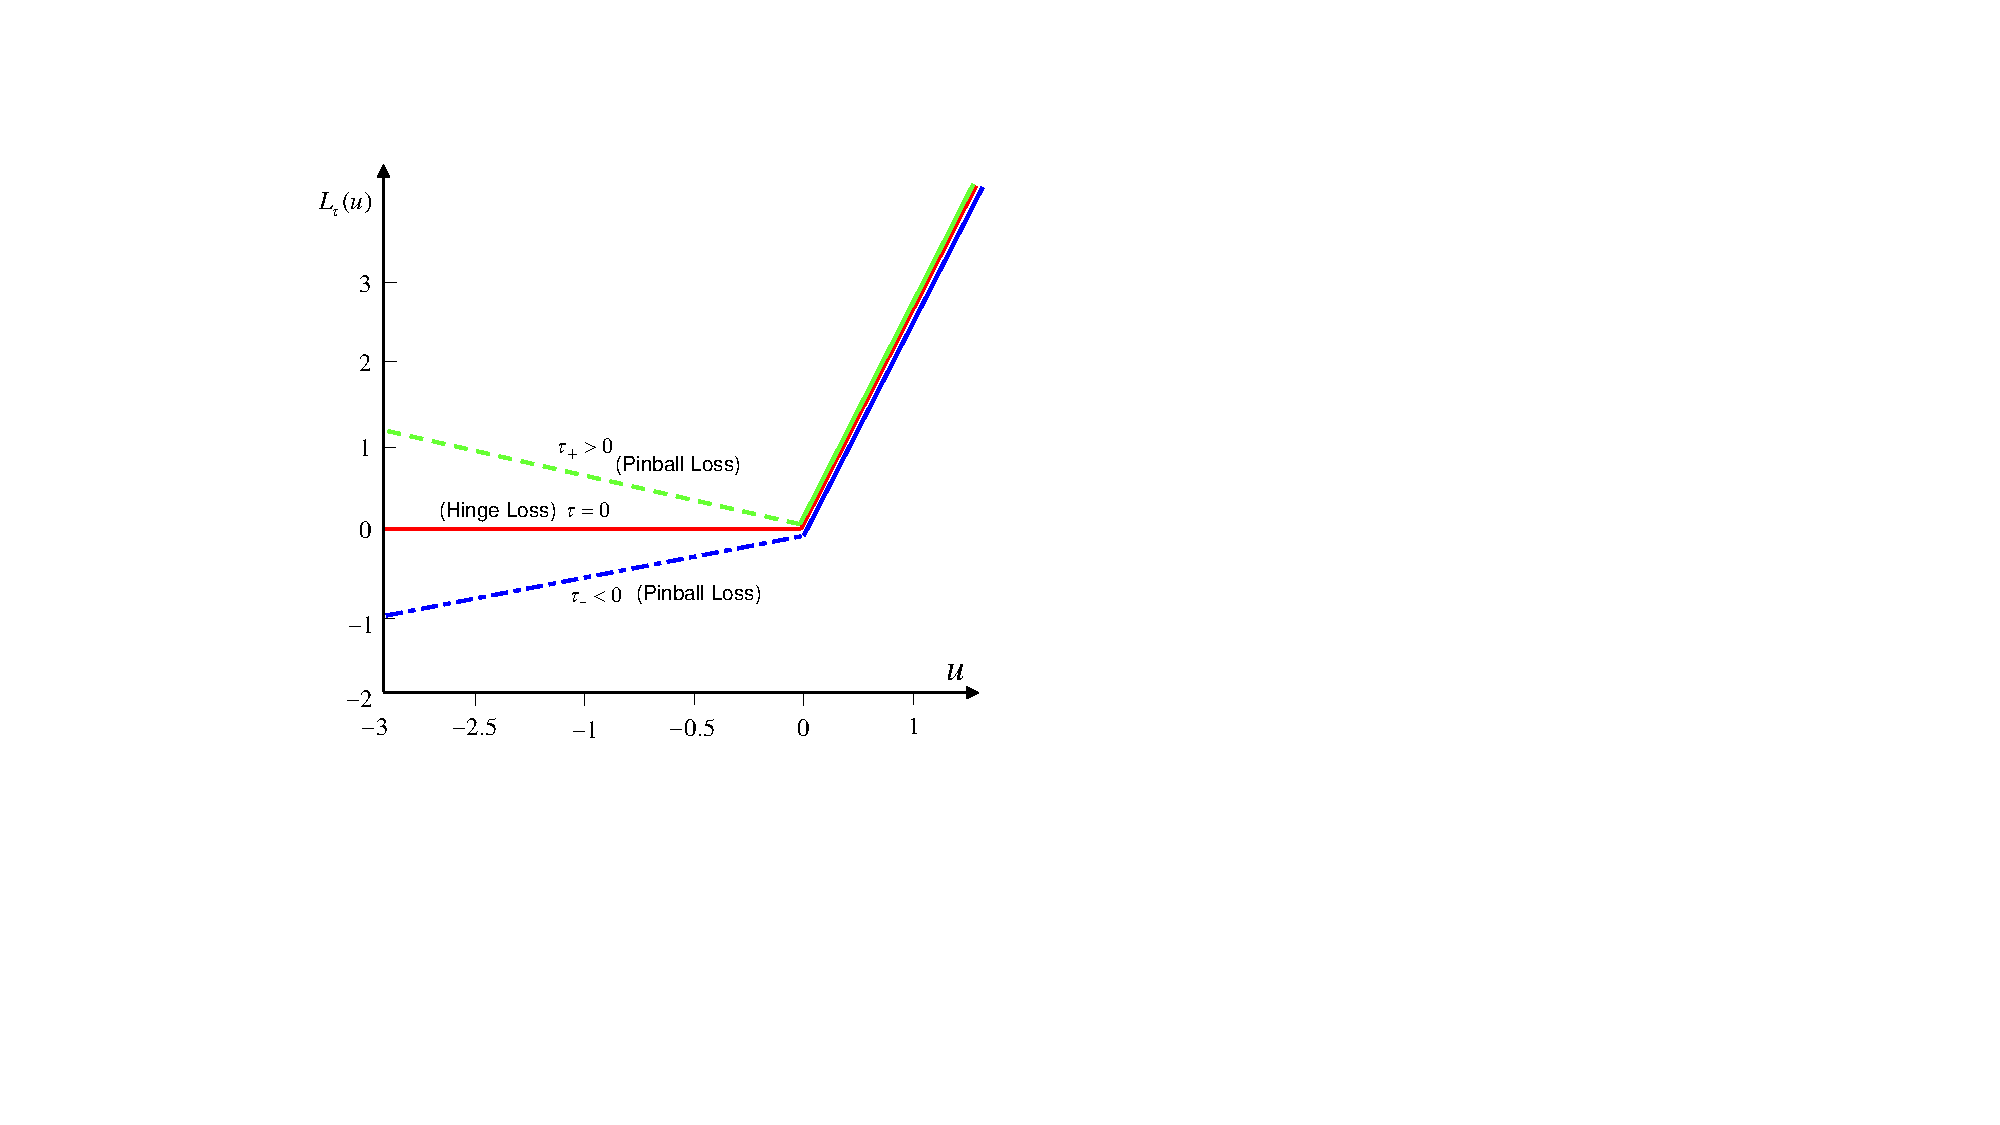
\includegraphics[width=8cm]{loss.pdf}
	\caption{Comparison of loss functions  $L_{ hinge }(u)$ and $L_{\tau }(u)$.}
		\label{loss}
\end{figure}
\vspace{2mm}


According to Anand et al., when $\tau$ is positive or negative, the classifier model is inconsistent \citep{anand2021improvement}. Therefore, we refer to the pinball loss that applies to both positive and negative values as UP loss. Denote $u=1-y\left(w^{T} x+b\right)$, and it represents the distance from the sample point to the hyperplane of this class for SVM. As can be seen from Fig. \ref{loss}, when $u>0$, it means that the sample points appear between the positive and negative hyperplanes. In this case, both hinge loss and UP loss will punish these samples in unit rate. When $u<0$, it means that the sample points are correctly classified and appear outside the hyperplane. In this case, the penalty given to these samples by hinge loss is 0, but UP loss will also give these samples a penalty at a relatively low rate $\tau$. The above difference shows that hinge loss only focuses on these samples that appear between the positive and negative hyperplanes, while the UP loss takes into account all sample points and is less sensitive to noise.

Theory and experiments prove that, compared with hinge loss, UP loss can bring better classification performance to SVM. By replacing hinge loss with UP loss, we can get the linearized UPSVM model as follows
\begin{equation}
\begin{aligned}
& \min _{w, b} \frac{1}{2}\|w\|^{2}+C_{0} \sum_{i=1}^{l} L_{\tau}\left(1-y_{i}\left(w^{T} x_{i}+b\right)\right),
\end{aligned}
\end{equation}
which is equivalent to

\begin{equation}
\begin{aligned}
\label{upsvm}
\min _{w, b} \frac{1}{2}\|w\|^{2} + C_{0} \sum_{i=1}^{l} &(\operatorname { m a x } \{1-y_{i}(w^{T} x_{i}+b),\\
-\tau(1-y_{i}(w^{T} x_{i}+b))\}),
\end{aligned}
\end{equation}
in Eq. (\ref{upsvm}), Pin-SVM and traditional SVM can be recovered by letting $\tau \geq 0$ and $\tau=0$, respectively.

% Additionally, considering the influence of imbalanced data, we allow the penalty term $C_i$ varies among different data points, which is actually a cost-sensitive strategy. 
% Denote $u_i$ as the distance between the the sample point and the corresponding hyperplane, i.e., $u_i=1-y_{i}(w^{T} x_{i}+b)$. Then
\section{DBUPLDM}\label{3}
When dealing with imbalanced datasets, models are often affected by this imbalance to varying degrees. Since the LDM needs to maximize the mean margin, the classification hyperplane is skewed toward a class with a small size, which reduces the model's ability to generalize to samples from imbalanced datasets. Firstly, a new dual balanced factor function is introduced in subsection \ref{dbb}.
Based on the dual balance function and UP loss function, we propose the DBUPLDM model in subsection \ref{3.1}. In subsection \ref{3.2}, we present the explicit solution to DBUPLDM and provide the derivation in detail. 

\subsection{Dual balance } \label{dbb}
This subsection proposes a novel balance factor to measure the degree of imbalance, from which the composite distance is constructed.

\begin{myDef}\label{pf}
The penalty function of DBUPLDM is defined as:
\begin{equation}
{C_i}^* = \left\{ \begin{array}{l}
{C_0},{x_i} \in {{Small \  Category}}\\
k{C_0},{x_i} \in {{Large \ Category}}
\end{array} \right.,
\end{equation}
where $k = {{\min ({\psi ^ - },{\psi ^ + })} \mathord{\left/
 {\vphantom {{\min ({\psi ^ - },{\psi ^ + })} {\max ({\psi ^ - },{\psi ^ + })}}} \right.
 \kern-\nulldelimiterspace} {\max ({\psi ^ - },{\psi ^ + })}}.$
\end{myDef}

From Definition \ref{pf}, it can be seen that $k$ is used to denote the proportion of imbalanced categories and can measure the magnitude of this bias. $k$ is always a value less than one, thus reducing the penalty of large category samples in slack and increasing the penalty factor of small category samples. Therefore, the relaxation of the small category samples is suppressed and their importance is enhanced.

\begin{myDef}\label{bf}
Define the balance factor as:
\begin{equation}
{\theta _i} = 1 \pm (\frac{1}{k}){^\rho }\frac{{\left| {{\psi ^ - } - {\psi ^ + }} \right|}}{{{\psi ^ - } + {\psi ^ + }}},
\end{equation}
where $\psi$ represents the number of samples and $\rho$ is an adjustable parameter that controls the sensitivity of the balance factor to class imbalance. 

\end{myDef}
 
Definition \ref{bf} presents the balance factor function. {\color{orange}In practical applications, we empirically set $\rho = 1/2$, as this value provides moderate nonlinearity in the scaling process and ensures stable model performance across various datasets. Users can tune $\rho$ within the range $[0, 1]$ according to the imbalance degree of the dataset.
\begin{remark}\label{remark 1}
The tuning of \(\rho\) depends on the dataset's imbalance degree, and specific guidelines are as follows:\begin{itemize}\item \textbf{Low Imbalance Scenarios (e.g., class sample ratio ratio \(\leq 10:1\))}:Restrict \(\rho\) to the range \(0.4\)--\(0.6\) to prevent performance degradation of majority-class samples caused by excessive intervention.\item \textbf{High Imbalance Scenarios (class sample ratio \(> 10:1\))}:Increase \(\rho\) appropriately to the range \(0.6\)--\(0.7\) to enhance the protection of minority-class samples by improving sensitivity.\item \textbf{Critical Note}:\(\rho\) is not advisable to exceed \(0.8\); otherwise, the classification accuracy of majority-class samples may drop sharply due to over-amplified nonlinear effects.\end{itemize}\end{remark}
For a detailed sensitivity analysis of $\rho$, we verify its impact through experiments in Supplementary 3. Specifically, we test the model performance with different values of $\rho$ on two representative imbalanced datasets (covering scenarios with varying imbalance degrees), and the detailed experimental results are provided in the Supplementary.}

For imbalanced datasets, the classification hyperplane will be biased towards small class samples, which reduces the generalization performance. The balance factor function is used to adjust for this undesirable effect. For large class samples, the balance factor function generates an indicator variable greater than zero and less than one. On the other hand, for small class samples, it generates a variable greater than 1. For different situations, the balance factor function can be expanded as:
\begin{equation}
{\theta _i} = \left\{ \begin{array}{l}
{{1 + y_i{{({{{\psi ^ - }} \mathord{\left/
 {\vphantom {{{\psi ^ - }} {{\psi ^ + }}}} \right.
 \kern-\nulldelimiterspace} {{\psi ^ + }}})}^\rho }({\psi ^ - } - {\psi ^ + })} \mathord{\left/
 {\vphantom {{1 + y(i){{({{{\psi ^ - }} \mathord{\left/
 {\vphantom {{{\psi ^ - }} {{\psi ^ + }}}} \right.
 \kern-\nulldelimiterspace} {{\psi ^ + }}})}^\rho }({\psi ^ - } - {\psi ^ + })} {({\psi ^ + } + {\psi ^ - }),0 < {\psi ^ + } < {\psi ^ - }}}} \right.
 \kern-\nulldelimiterspace} {({\psi ^ + } + {\psi ^ - }),0 < {\psi ^ + } < {\psi ^ - }}}\\
{{1 - y_i{{({{{\psi ^ + }} \mathord{\left/
 {\vphantom {{{\psi ^ + }} {{\psi ^ - }}}} \right.
 \kern-\nulldelimiterspace} {{\psi ^ - }}})}^\rho }({\psi ^ + } - {\psi ^ - })} \mathord{\left/
 {\vphantom {{1 - y(i){{({{{\psi ^ + }} \mathord{\left/
 {\vphantom {{{\psi ^ + }} {{\psi ^ - }}}} \right.
 \kern-\nulldelimiterspace} {{\psi ^ - }}})}^\rho }({\psi ^ + } - {\psi ^ - })} {({\psi ^ + } + {\psi ^ - }),0 < {\psi ^ - } < {\psi ^ + }}}} \right.
 \kern-\nulldelimiterspace} {({\psi ^ + } + {\psi ^ - }),0 < {\psi ^ - } < {\psi ^ + }}}
\end{array} \right..
\end{equation}


\begin{myDef} 
The composite distance is defined as:
\begin{equation}
\gamma ^*={{\theta _{\rm{i}}}{y_i}{\omega ^T}\phi ({x_i})}
\label{cd}
\end{equation}
\end{myDef}

{\color{blue}The composite distance reconstructs the contribution of samples to the margin mean via the balance factor $\theta_i$. It assigns a larger weight to small class samples ($\theta_i$ > 1) and a smaller weight to large class samples ($\theta_i \in (0,1)$), adjusting the effective distances of the two classes. Thus, it balances the hyperplane and corrects the problem of its tilting toward small class samples in imbalanced data.}

{\color{magenta}
\begin{remark}[Terminology Clarification]
To ensure clarity and consistency throughout this paper, we distinguish between two key distance concepts:
\begin{itemize}
    \item \textit{Quantile Distance}: This refers to the distance measure induced by the unified pinball loss function, which is related to the $\tau$-quantile of the residual distribution. Unlike the traditional Euclidean distance used in SVM's hinge loss, quantile distance provides robustness against outliers and noise by focusing on specific quantiles of the error distribution rather than the worst-case error.
    \item \textit{Composite Distance}: This refers to the dual-balanced distance defined in Definition 3, which combines the imbalance ratio and the bias factor through the balance function $\theta_i$. The composite distance modifies the margin calculation for majority and minority classes separately, ensuring a balanced classification hyperplane.
\end{itemize}
These two concepts work synergistically in DBUPLDM: the quantile distance (through UP loss) provides noise immunity, while the composite distance (through dual-balanced mechanism) addresses class imbalance. Together, they form the foundation of DBUPLDM's superior performance on imbalanced and noisy datasets.
\end{remark}
}



Considering that $\theta_{i}$ is a segmented function, bringing it into Eq. (\ref{cd}), the form of the composite distance can be written as:

\begin{equation}
\begin{aligned}
& {\gamma ^*} = {\theta _{\rm{i}}}{y_i}{\omega ^T}\phi ({x_i}) = (1 \pm {\Delta}){y_i}{\omega ^T}\phi ({x_i}) = \gamma  \pm {\Delta}{y_i}{\omega ^T}\phi ({x_i}),\\
& {\Delta} = (\frac{1}{k})^{\rho}\frac{{\left| {{\psi ^ - } - {\psi ^ + }} \right|}}{{{\psi ^ - } + {\psi ^ + }}}
\end{aligned}
\end{equation}

After replacing the original distance with the composite distance, the margin mean is transformed into:
\begin{equation}
{\gamma _1}^* = \sum\limits_{i = 1}^m {{\theta _{\rm{i}}}{y_i}{\omega ^T}\phi ({x_i}) = } \sum\limits_{i = 1}^m {(1 \pm {\Delta}){y_i}{\omega ^T}\phi ({x_i})}  = \gamma  \pm \sum\limits_{i = 1}^m {{\Delta}{y_i}{\omega ^T}\phi ({x_i})} 
\end{equation}

\begin{figure} [H]
    \centering
    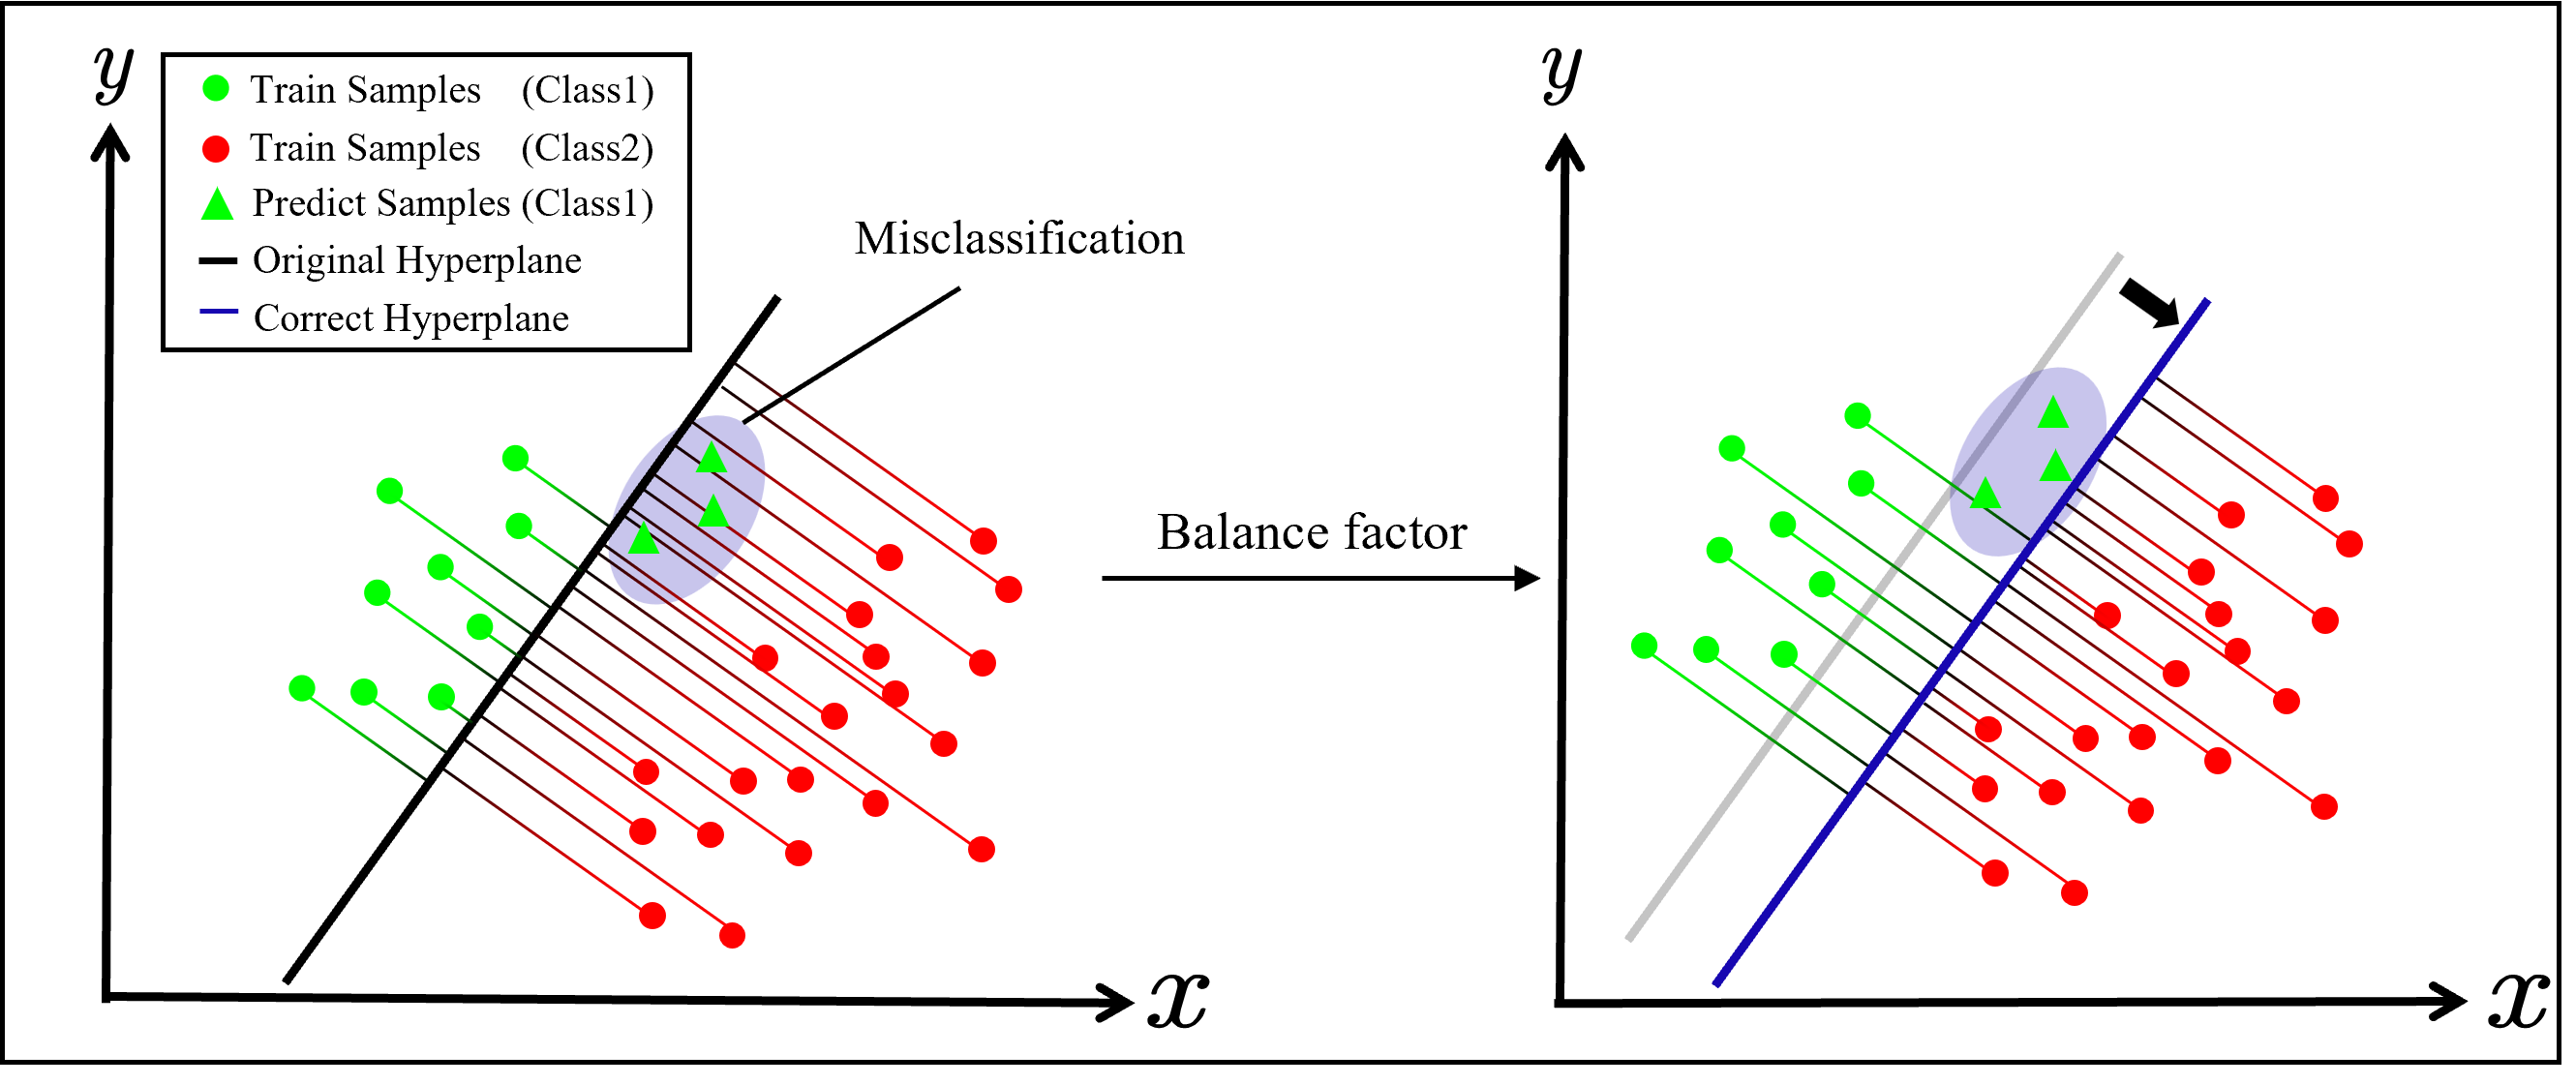
\includegraphics[width=15cm]{Figure/fig_2.png}
    \caption{\color{blue}Demonstration of the effect of balance factors. It can be clearly seen that the classification hyperplane will no longer tilt towards minority classes, and the number of misclassified classes in minority classes will be greatly reduced.}\label{bff}
\end{figure}

According to Eq. (\ref{mean}), the matrix form of ${\gamma _1}^*$ can be written as:
\begin{equation}
{\gamma _1}^* = \frac{1}{m}{(X{\bf{\theta }}Y)^T}\omega,
\end{equation}
where ${\bf{\theta }} = diag[{\theta _1},{\theta _2},...,{\theta _m}]$.
The effect of the balance factor can be represented by Fig. \ref{bff}.


By constructing the composite distance through the balance factor function, the distance of the small class samples will become larger, while the distance of the large class samples will become smaller subsequently. In this way, the classification hyperplane can be in a balanced state during the training process, and will not be affected by the imbalanced data on both sides.


\subsection{Model construction}\label{3.1}
As we mentioned earlier, LDM considers the margin distribution of all samples and has better generalization ability, i.e., it also inherits the hinge loss of SVM. LDM with hinge loss only requires a certain penalty to points located between positive and negative hyperplanes, and the penalty parameters of other points are 0, which causes LDM to be sensitive to noise and unstable resampling. Therefore, we replaced traditional hinge loss with UP loss, providing a more subtle penalty mechanism and improving robustness. 

% As shown in the Fig. \ref{dbup}, the UP loss adopts quantile distance instead of the shortest distance, thereby reducing sensitivity to noise.


% \begin{figure*} 
%     \centering
%     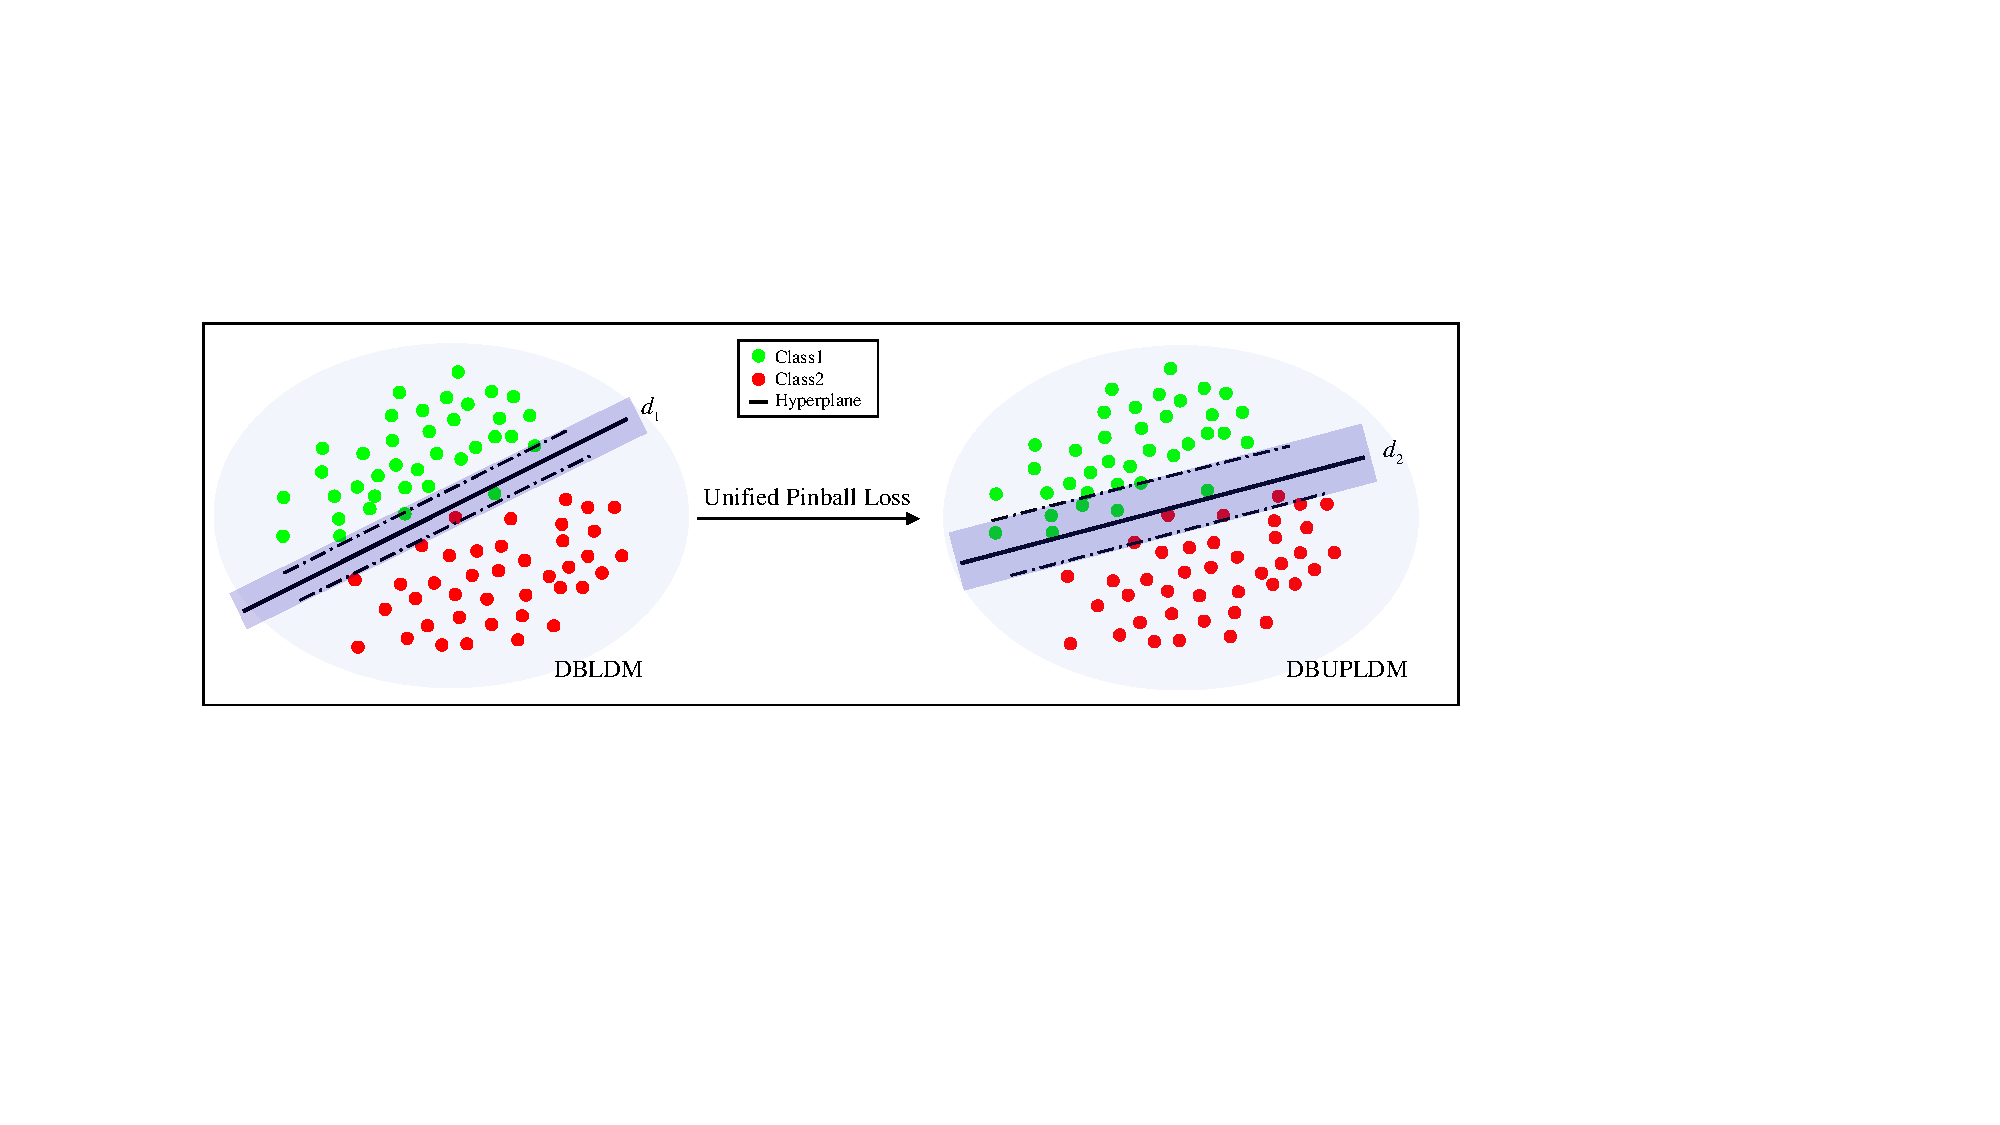
\includegraphics[width=15cm]{Demonstration0.pdf}
%     \caption{Comparison of DBLDM and DBUPLDM. The quantile distance of UP loss replaces the traditional shortest distance in LDM, which helps to improve the anti-interference ability of the model.}
%     \label{dbup}

% \end{figure*}




To make improvements to the low generalization performance of the model in handling imbalanced data, we combine the idea of dual balance with UP loss and propose a novel dual balanced large margin classifier (called DBUPLDM), which is formulated as
\begin{equation}\label{UPLDM1}
\begin{aligned}
\min _{w, b} \frac{1}{2}\|w\|^{2} -\lambda_{1} {\gamma _1}^*+\lambda_{2} \gamma_{2}+ \sum_{i=1}^{l} \theta_{i}P_{\tau}\left(1-y_{i}\left(w^{T} x_{i}+b\right)\right),
\end{aligned}
\end{equation}
where $P_{\tau}$ is a cost-sensitive UP loss function. As a cost-sensitive quantile distance, $P_{\tau}(u_i)$ is expressed as
\begin{equation}\label{UP}
P_{\tau}(u_i)={C_i}^* L_{\tau}(u_i) =\max \{u_i{C_i}^*, -\tau u_i {C_i}^*\},
\end{equation}
where $\tau \in [-1,1]$ is the parameter that determines the quantile level. Introducing the slack variable $\xi_i=L_{\tau}(1-y_{i}(w^{T} x_{i}+b)$, the equivalent form of Eq. (\ref{UPLDM1}) can be rewritten as
\begin{equation}\label{DBUPLDM2}
\begin{aligned}
\min _{w,b,\xi} & \frac{1}{2}\|w\|^{2}-\lambda_{1} {\gamma _1}^*+\lambda_{2} \gamma_{2}+\sum_{i=1}^{l} \rho_{i}\theta_{i} \xi_{i} \\
\text { s.t. } \quad & \xi_{i} \geq 1-y_{i}\left(w^{T} x_{i}+b\right), \\
& \xi_{i} \geq-\tau\left(1-y_{i}\left(w^{T} x_{i}+b\right)\right), i=1, \ldots, l.
\end{aligned}
\end{equation}
% \begin{equation}\label{DBUPLDM2}
% \begin{aligned}
% \min _{w,b,\xi} & \frac{1}{2}\|w\|^{2}-\lambda_{1} {\gamma _1}^*+\lambda_{2} \gamma_{2}+\sum_{i=1}^{l} C_is_{i} \xi_{i} \\
% \text { s.t. } \quad & \xi_{i} \geq 1-y_{i}\left(w^{T} x_{i}+b\right), \\
% & \xi_{i} \geq-\tau\left(1-y_{i}\left(w^{T} x_{i}+b\right)\right), i=1, \ldots, l.
% \end{aligned}
% \end{equation}
By utilizing a kernel function, the input data is mapped to the Hilbert space $\mathbb{H}$ through a typical nonlinear mapping. Assuming that the data point ${x_i}$ is mapped from $\mathbb{R}^{n}$ to $\mathbb{R}^{e}(e>n)$, the relationship can be expressed as $\phi: X \rightarrow \mathbb{H}$. Letting $D=y_{i}\left(w^{T} \phi( x_{i})+b\right)$, we can get the objective function for the nonlinear case of the proposed DBUPLDM model
\begin{equation}
\label{qpp}
\begin{aligned}
\min _{w, b, \xi} & \frac{1}{2}\|w\|^{2}-\lambda_{1} {\gamma _1}^*+\lambda_{2} \gamma_{2}+\sum_{i=1}^{l} \rho_{i}\theta_{i} \xi_{i} \\
\text { s.t. } & \xi_{i} \geq 1-D_{i}, \\
\quad & \xi_{i} \geq-\tau\left(1-D_{i}\right), i=1, \ldots, l,
\end{aligned}
\end{equation}
where $\gamma_{1}=\frac{1}{l} \sum_{i=1}^{l} D_{i}$ and $\gamma_{2}=\sum_{i=1}^{l} \sum_{j=1}^{l}\left(D_{i}-D_{j}\right)^{2}$.
{\color{blue}The joint objective function of DBUPLDM is convex, as it comprises a quadratic term for the margin maximization and linear constraints, ensuring a unique global optimum. This convexity guarantees the optimization problem's stability and solvability using standard quadratic programming techniques.}

\begin{remark}
The performance of DBUPLDM will be affected by the value of $\tau$ and the balance factor. The proposed DBUPLDM model is a general version of LDM and SVM models.
\item[$\bullet$] when $\tau = 0$, the proposed DBUPLDM is degenerated into a dual balanced LDM model with hinge loss.
\item[$\bullet$] When $\theta_i=1$ (i=1, 2, \ldots, l) and $\tau \geq 0$, the proposed DBUPLDM is degenerated into a LDM model with pinball loss, which can be called Pin-LDM.
\item[$\bullet$] When $\lambda_{1} = \lambda_{2} = 0$ and $\theta_i=1$, the proposed DBUPLDM is degenerated into UPSVM \citep{anand2021improvement}.
\item[$\bullet$] When $\lambda_{1} = \lambda_{2} = 0$, and $\tau \geq 0$, the proposed model is degenerated into Pin-SVM \citep{huang2013support,huang2016solution}.
\end{remark}

{\color{red}We stress that DBUPLDM is not a direct combination of existing ingredients: its innovation lies in how imbalance and noise are jointly addressed through a redefined margin within a single LDM. First, none of the existing methods redefines the margin itself for imbalance: Gu et al.'s twin bounded classifier~\citep{gu2024twin} keeps the margin definition unchanged in a twin framework, while CS-LDM~\citep{cheng2016cost} adjusts the margin with a coefficient built from class counts alone, ignoring the bias term and leaving majority-class samples untreated. Our dual balanced composite distance is new in coupling the imbalance ratio with the bias term and in treating both classes explicitly ($\theta_i>1$ for minority samples and $\theta_i\in(0,1)$ for majority samples), and it enters both the margin mean and the second-order statistics of the LDM. Second, the integration itself is non-trivial: reshaping the margin distribution while replacing the hinge loss with the UP loss leads to a new QPP whose explicit solution is derived in Section~\ref{3.2}, and the resulting model unifies several existing models as special cases (dual balanced LDM with hinge loss, Pin-LDM, UPSVM, and Pin-SVM).}

% (DBUPLDM UPLDM UPSVM PinSVM SVM)
%  when $\rho_{i}=C_{0}$ (i=1, \ldots, l), the proposed DBUPLDM model is degenerated into a cost-insensitive model, which can be called UP-LDM.

\subsection{QPP for solving DBUPLDM problem}\label{3.2}
Introducing Lagrange multipliers $\alpha_{i}$ and $\beta_{i}$, the Lagrangian function  associated with Eq. (\ref{qpp}) is
\begin{equation}
\label{qpp2}
\begin{aligned}
&\mathrm{L}(w, b, \xi ; \alpha, \beta)=\frac{1}{2}\|w\|^{2}-\frac{\lambda_{1}}{l} \sum_{i=1}^{l} D_{i} \\
&+\lambda_{2} \sum_{i=1}^{l} \sum_{j=1}^{l}\left(D_{i}-D_{j}\right)^{2}+\sum_{i=1}^{l} \rho_{i}\theta_{i} \xi_{i} \\
&-\sum_{i=1}^{l} \alpha_{i}\left(D_{i}+\xi_{i}-1\right)-\sum_{i=1}^{l} \beta_{i}\left(\tau\left(1-D_{i}\right)+\xi_{i}\right).
\end{aligned}
\end{equation}

Since it is very difficult to directly handle the Lagrangian function in Eq. (\ref{qpp2}), we below convert it to matrix form. 
{\color{blue}The DBUPLDM optimization problem exhibits guaranteed convergence due to the convexity of the objective function and the use of standard quadratic programming solvers,  ensuring stable and efficient solutions. Iterative optimization methods, such as sequential minimal optimization, further enhance convergence speed for large-scale imbalanced datasets.}
\begin{myTheo}
\label{theo1}
The optimal solution $w^*$ for Eq. (\ref{qpp}) admits a representation of the form:
\begin{equation}
\label{thor}
\boldsymbol{w}^{*}=\sum_{i=1}^{l} \delta_{i} \phi\left(\boldsymbol{x}_{i}\right)=\Phi \boldsymbol{\delta},
\end{equation}
where $\boldsymbol{\delta}=\left[\delta_{1}, \ldots, \delta_{l}\right]^{T}$ is a vector by stacking the specific coefficients and $\Phi=\left[\phi_{1}, \ldots, \phi_{l}\right]^{T}$.
\end{myTheo}

\begin{proof}
The proof of this theorem refers to \citep{smola2002support}.
\end{proof}

By applying Theorem \ref{theo1}, one can establish the following equalities
\begin{equation}
\label{thor2}
\begin{aligned}
&\sum_{i=1}^{l} {D}_{i}\mathrm{\theta_i} =l \gamma_{1}^*, \\
&\gamma_{1}^* =\frac{1}{l} \sum_{i=1}^{l} {D}_{i}\mathrm{\theta_i}=\frac{1}{l} (\mathbb{\theta}Y)^{T} K \delta, \\
&\gamma_{2} =\sum_{i=1}^{l} \sum_{j=1}^{l}\left(D_{i}-D_{j}\right)^{2} \\
&=\frac{2 \delta^{T} K K^{T} \delta}{l}-\frac{2 \delta^{T} K Y Y^{T} K \delta}{l^{2}},
\end{aligned}
\end{equation}
where the kernel function $K = {\Phi^T}\Phi$, and $Y$ is the label vector of the sample. The Gaussian kernel function can be expressed as
\begin{equation}
\label{gaosikenl}
K\left(x_{i}, x_{j}\right)=\exp \left(\frac{-\left\|x_{i}-x_{j}\right\|_{2}}{2 \sigma^{2}}\right),
\end{equation}
where $\sigma$ is known as the width parameter, see \citep{scholkopf2002learning}. For the linear kernel, $K = x_{i}^{T} x_{j}$. 

% Recall that the Gaussian kernel function can
% For Gaussian kernel, $K = \exp \left(\frac{-\left\|x_{i}-x_{j}\right\|_{2}}{2 \sigma^{2}}\right)$;


Substituting Eq. (\ref{thor}) and Eq. (\ref{thor2}) into Eq. (\ref{qpp}) gives
\begin{equation}
\label{matrix}
\begin{aligned}
\min _{\delta, \xi} & \frac{1}{2} \delta^{T} Q \delta+E^{T} \delta+\sum_{i=1}^{l} \rho_{i}\theta_{i}  \xi_{i} \\
\text { s.t. } & \xi_{i} \geq 1-D_{i}, \\
& \xi_{i} \geq-\tau\left(1-D_{i}\right), i=1, \ldots, l,
\end{aligned}
\end{equation}
where 
\begin{equation}
\label{computeQE}
\begin{aligned}
&Q=4 \lambda_{2}\left(l K^{T} K-(K Y)(K Y)^{T}+4 \lambda_{2} l^{2} K\right) / l^{2}, \\
&E=-\lambda_{1} K\mathbb{\theta}Y / l.
\end{aligned}
\end{equation}

The following theorem presents the fundamental dual problem formulation for DBUPLDM, which is central to our model's optimization strategy and theoretical foundation.

\begin{myTheo}
\label{theo2}
The dual problem of the DBUPLDM optimization problem (Eq. (\ref{matrix})) admits a representation of the form: 
\begin{equation}
\label{dual}
\begin{aligned}
\min _{\boldsymbol{\alpha, \hat{\beta}}} \frac{1}{2}( & \boldsymbol{\alpha}-v \boldsymbol{\hat{\beta}})^{T} A(\boldsymbol{\alpha}-v \boldsymbol{\hat{\beta}})+\left(\frac{\lambda_{1} A\mathbb{\theta}e-l e}{l}\right)^{T}(\boldsymbol{\alpha}-v \boldsymbol{\hat{\beta}}) \\
\text { s.t. } \quad & \alpha_{i}+\frac{\hat{\beta_{i}}}{|\tau|}=\rho_{i}, \\
& \alpha_{i} \geq 0, \hat{\beta_{i}} \geq 0, i=1, \ldots, l,
\end{aligned}
\end{equation}
where $\boldsymbol{\alpha}=[\alpha_{1},\alpha_{2},...,\alpha_{l}]^{T}$ and $\boldsymbol{\hat{\beta}}=[\hat{\beta}_{1},\hat{\beta}_{2},...,\hat{\beta}_{l}]^{T}$, $v$ is an indicator function.
\end{myTheo}

\begin{proof}
{\color{orange}See Supplementary 4 for details.}
% Combine Eq. (\ref{thor2}), the Lagrangian function of Eq. (\ref{matrix}) is

% \begin{equation}
% \begin{aligned}
% \label{laa}
% &L(\delta,\xi ;\alpha ,\beta ) = \frac{1}{2}{\delta ^T}Q\delta  + {E^T}\delta  + \sum\limits_{i = 1}^{l} \rho_{i}\theta_{i} \xi _{i} \\
%  &- \sum\limits_{i = 1}^l {{\alpha _i}({\xi _i} + {y_i}{\delta ^T}{K_i} - 1)}- \sum\limits_{i = 1}^l {{\beta _i}({\xi _i} + \tau (1 - {y_i}{\delta ^T}{K_i}))} .
% \end{aligned}
% \end{equation}

% According to the Karush–Kuhn–Tucker (KKT) optimization condition, the following equations can be obtained
% \begin{equation}
% \label{kkt}
% \begin{aligned}
% &\frac{\partial L}{\partial \delta}=Q \delta+E-\sum_{i=1}^{l} \alpha_{i} y_{i} K_{i}+\tau \sum_{i=1}^{l} \beta_{i} y_{i} K_{i}=0, \\
% &\frac{\partial L}{\partial \xi_{i}}=\rho_{i}\theta_{i}-\alpha_{i}-\beta_{i}=0, \forall i=1,2, \ldots, l .
% \end{aligned}
% \end{equation}

% Therefore, the dual problem of the original Eq. (\ref{matrix})  is
% \begin{equation}
% \label{opti}
% \begin{aligned}
% \min _{\boldsymbol{\alpha, \beta}} \frac{1}{2}( & \boldsymbol{\alpha}-\tau \boldsymbol{\hat{\beta}})^{T} A(\boldsymbol{\alpha}-\tau \boldsymbol{\hat{\beta}})+\left(\frac{\lambda_{1} A\mathbb{\theta}e-l e}{l}\right)^{T}(\boldsymbol{\alpha}-\tau \boldsymbol{\hat{\beta}}) \\
% \text { s.t. } \quad & \alpha_{i}+\beta_{i}=\rho_{i}, \\
% & \alpha_{i} \geq 0, \beta_{i} \geq 0, i=1, \ldots, l,
% \end{aligned}
% \end{equation}
% where 

% \begin{equation}
% \label{computeA}
% \begin{aligned}
% &A=[\operatorname{diag}(Y)] K Q^{-1} K[\operatorname{diag}(Y)], \\
% &e=[1, \ldots, 1]_{1 \times m}.
% \end{aligned}
% \end{equation}

% It can be seen from the Eq. (\ref{opti}) that when $\tau$ is negative, the final optimization problem of the model is different from that when $\tau$ is positive. This proves that Huang et al.'s method of extending $\tau$ to negative values \citep{huang2016solution} is wrong.

% We define the signum function $v_{u}$ by
% \begin{equation}
% v_{u}=\left\{\begin{array}{l}
% 1 \quad \text { if } u \geq 0, \\
% -1 \quad \text { otherwise, }
% \end{array}\right.
% \end{equation}
% and let $\hat{\beta}=|\tau| \beta$ , then the dual Eq. (\ref{opti}) can be given by
% \begin{equation}
% \label{dual}
% \begin{aligned}
% \min _{\boldsymbol{\alpha, \hat{\beta}}} \frac{1}{2}( & \boldsymbol{\alpha}-v_{\tau} \boldsymbol{\hat{\beta}})^{T} A(\boldsymbol{\alpha}-v_{\tau}\boldsymbol{\hat{\beta}})+\left(\frac{\lambda_{1} A\mathbb{\theta}e-l e}{l}\right)^{T}(\boldsymbol{\alpha}-v_{\tau} \boldsymbol{\hat{\beta_{j}}}) \\
% \text { s.t. } \quad & \alpha_{i}+\frac{\hat{\beta_{i}}}{|\tau|}=\rho_{i}, \\
% & \alpha_{i} \geq 0, \hat{\beta_{i}} \geq 0, i=1, \ldots, l.
% \end{aligned}
% \end{equation}
\end{proof}

Again, we observe the equivalence between the traditional LDM and the DBUPLDM with $\tau$ = 0: when $\tau$ is small enough, $\frac{\hat{\beta}}{|\tau|}$ can provide any positive value, thus the corresponding constraint is satisfied if and only if $-v\left| \tau \right|\rho_{i}\theta_{i} \leq \alpha_{i} \leq \rho_{i}\theta_{i}$. Hence, Eq. (\ref{dual}) reduces to the dual formulation of the hinge loss LDM
\begin{equation}
\label{ldmdual}
\begin{aligned}
\min _{\boldsymbol{\alpha}} & \frac{1}{2} \boldsymbol{\alpha}^{T} A \boldsymbol{\alpha}+\left(\frac{\lambda_{1} A\mathbb{\theta}e-l e}{l}\right)^{T} \boldsymbol{\alpha} \\
\text { s.t. } \quad &  -v\left| \tau \right|\rho_{i}\theta_{i} \leq \alpha_{i} \leq \rho_{i}\theta_{i}, i=1, \ldots, l.
\end{aligned}
\end{equation}

After obtaining the solution ($\alpha^{*}, \beta^{*}$) of the dual problem (Eq. (\ref{dual})), $\delta$ can be given by
\begin{equation}
\label{delta}
\begin{aligned}
&\delta  = {Q^{ - 1}}\left\{ {K[diag(Y)](\alpha^{*}  - v_{\tau}\hat{\beta}^{*}) - E} \right\}\\
% & \ \ = {Q^{ - 1}}\left\{ {\frac{{{\lambda _1}}}{l}K[diag(Y)]e + K[diag(Y)](\alpha^{*}-v_{\tau}\hat{\beta}^{*}) } \right\}\\
& \ \ = {Q^{ - 1}}K[diag(Y)](\frac{\lambda_{1}\mathbb{\theta}e}{m}+\alpha^{*}-v_{\tau}\hat{\beta}^{*}).
\end{aligned}
\end{equation}

For a given test point $x_z \in \mathbb{R}^{n}$, the decision function is obtained as
\begin{equation}
\label{juece}
f(x_z) = {\mathop{\rm sgn}} ({w ^T}\phi ({x_z})) = {\mathop{\rm sgn}}(\sum\limits_{i = 1}^l {{\delta _i}K({x_i},x_z)} ).
\end{equation}

Once the decision function of DBUPLDM is obtained, the categorization task can be performed by Eq. (\ref{juece}) for a new test sample.



\renewcommand{\thesection}{\color{blue}\arabic{section}}
\section{\textcolor{blue}{Properties of DBUPLDM \label{4}}}% Numbering is blue
\renewcommand{\thesection}{\arabic{section}}


\begin{color}{blue}
\textbf{\textit{A.Noise Insensitivity}}

 Since DBUPLDM uses the UP loss function, it can weaken the sensitivity to noise around the decision boundary.
The segmented function $\text{sgn}_\tau (u)$ is defined as:

\begin{equation}
\text{sgn}_\tau (u) = \begin{cases} 
1 & \text{if } u > \tau, \\
0 & \text{if } |u| \leq \tau, \\
-1 & \text{if } u < -\tau.
\end{cases}
\label{eq:sgn_function} 
\end{equation}
where  $\text{sgn}_\tau (u)$ is the subgradient of UP loss $P_{\tau}(u_i)$. Without loss of generality, we focus on a linear classifier. Denote 0 as an all-zero vector, then the optimal condition of optimization problem (\ref{UPLDM1}) can be written as:

\begin{equation}
0 \in \omega + 2\lambda_{2} \sum_{i,j=1}^{l} (y_{i}x_{i} - y_{j}x_{j})(D_{i} - D_{j}) - \frac{\lambda_{1}}{l} \sum_{i=1}^{l} \theta_{i} y_{i}x_{i} - \sum_{i=1}^{l} \theta_{i} C_{i}^{*} \text{sgn}_{\tau}(1 - D_{i}) y_{i}x_{i}.
\label{eq:optimal_condition_dbupldm}
\end{equation}

To concretely explain the noise insensitivity of DBUPLDM, we divide the index set of samples into three disjoint subsets based on the relationship between \(1 - D_i\) and \(\tau\):

\begin{equation}
\begin{aligned}
U_{\omega,b}^{+} &= \left\{ i : 1 - D_i > \tau \right\}; \\
U_{\omega,b}^{0} &= \left\{ i : \vert 1 - D_i \vert \leq \tau \right\}; \\
U_{\omega,b}^{-} &= \left\{ i : 1 - D_i < -\tau \right\},
\end{aligned}
\label{eq:dbupldm_subsets}  
\end{equation}
where \(i = 1, \ldots, l\) and \(D_i = y_i(\omega^T x_i + b)\). Using Eq. (\ref{eq:dbupldm_subsets}) and the definition of \(\text{sgn}_\tau(u)\), we rewrite the optimal condition (\ref{eq:optimal_condition_dbupldm}) to analyze how noise affects the decision boundary.

Substituting the subsets \( U_{\omega,b}^{+}, U_{\omega,b}^{0}, U_{\omega,b}^{-} \) into Eq. (\ref{eq:optimal_condition_dbupldm}), the optimal condition becomes:

\begin{equation}
\begin{aligned}
\omega &+ 2\lambda_2 \sum_{i,j=1}^{l} (y_i x_i - y_j x_j)(D_i - D_j) - \frac{\lambda_1}{l} \sum_{i=1}^{l} \theta_i y_i x_i \\
&- \sum_{i \in U_{\omega,b}^{+}} \theta_i C_i^* \cdot 1 \cdot y_i x_i 
- \sum_{i \in U_{\omega,b}^{0}} \theta_i C_i^* \cdot 0 \cdot y_i x_i 
- \sum_{i \in U_{\omega,b}^{-}} \theta_i C_i^* \cdot (-1) \cdot y_i x_i = \boldsymbol{0}.
\end{aligned}
\label{eq:optimal_condition_expanded} 
\end{equation}

The above conditions indicate that $\tau$ controls the number of samples present in the sets $U_{\omega,b}^{+}$ and $U_{\omega,b}^{-}$.

\begin{remark}
The performance of DBUPLDM will be affected by the value of $\tau$.
\begin{itemize}
    \item \(\boldsymbol{\tau = 1}\):  
    The "insensitive zone" \(U_{\omega,b}^{0}\) shrinks (fewer samples satisfy \(|1 - D_i| \leq \tau\)). A small number of noises has negligible impact on the \emph{stable core gradient} in Eq. (\ref{eq:optimal_condition_expanded}):  
\begin{equation}
    \underbrace{\omega + 2\lambda_2 \sum_{i,j=1}^l (y_i x_i - y_j x_j)(D_i - D_j) - \frac{\lambda_1}{l} \sum_{i=1}^l \theta_i y_i x_i}_{\text{Stable Core Gradient, sign} = \chi}.
    \label{eq:stable_core_gradient}
\end{equation}  

Due to the large valid sample base, the model resists \textbf{zero-mean feature noise}, resulting in low sensitivity to such noise.  

    \item \(\boldsymbol{\tau}\) Decreases:  
    From the balanced relationship in Eq. (\ref{eq:optimal_condition_expanded}):  
\begin{equation}
    \sum_{i \in U_{\omega,b}^{+}} \theta_i C_i^* y_i x_i - \tau \sum_{i \in U_{\omega,b}^{0}} \theta_i C_i^* y_i x_i + \sum_{i \in U_{\omega,b}^{-}} \theta_i C_i^* y_i x_i = \frac{\chi}{l}.
\label{eq:balanced_relationship}
\end{equation}

As $tau$ decreases, \(U_{\omega,b}^{0}\) shrinks while \(U_{\omega,b}^{-}\) expands. Fewer samples in \(U_{\omega,b}^{+}\) concentrate noise influence, reducing noise insensitivity.  

    \item \(\boldsymbol{\tau < 0}\):  
    Correctly classified samples (in \(U_{\omega,b}^{0}\)) gain a \emph{distance bonus} via the negative branch of \(\text{sgn}_\tau(u)\) in Eq. (\ref{eq:optimal_condition_expanded}) when far from the boundary. This prioritizes distant samples, reducing reliance on noisy boundary-near points. Adjusting \(\tau < 0\) increases the average distance of correctly classified samples, significantly enhancing noise insensitivity.  
\end{itemize}
\end{remark}


\textbf{\textit{B.Imbalance Resilience}}

The core of DBUPLDM’s imbalance resistance in imbalanced classification lies in its dual - balancing mechanism, which fundamentally addresses traditional LDM’s neglect of small classes and over - dominance by large classes. It introduces the balancing factor to build composite distances, dynamically adjusting the two classes’ contributions to margin distribution.

\textbf{1. \(\boldsymbol{\theta}\) Influences the Optimization Direction of the Dual Objective through Vector \(\boldsymbol{E}\)}

The linear term of the dual problem in Eq.(\ref{thor2}) includes:
\begin{equation}
\left( \frac{\lambda_1 A \theta e - l \boldsymbol{e}}{l} \right)^T,
\label{eq:dual_linear_term}
\end{equation}
where \(\theta e\) is the cumulative vector of balancing factors, defined as \(\theta e = \left[ \sum \theta_1, \sum \theta_2, \cdots, \sum \theta_l \right]^T\)(\(\boldsymbol{e}\) denotes an all - one vector), and $A=[diag(Y)] K Q^{-1} K [diag(Y)]$.

For small class samples (\(\theta_i > 1\)): The corresponding components in \(\theta e\) are larger, making the "push" of the linear term \(\frac{\lambda_1 A \theta e}{l}\) stronger, guiding the dual variable \(\alpha - v_\tau \hat{\beta}\) to optimize in the direction of increasing the weight of small class samples;

For large class samples (\(0 < \theta_i < 1\)): The corresponding components in \(\theta e\) are smaller, weakening their contribution to the linear term and preventing the large class from overly dominating the dual optimization.

\textbf{2. \(\theta\) Composite Distance Reconstructs Matrices $Q$ and $A$ in the Dual Problem through 
Margin Mean $r_i^*$}

Through Eq. (\ref{thor2}), the margin mean \(\gamma_1^* = \frac{1}{l} (\theta Y)^T K \delta\) directly shapes the kernel matrix \(Q\) via its matrix form. According to $A = [\text{diag}(Y)]KQ^{-1}K[\text{diag}(Y)]$, \(\theta_i\) indirectly modulates \(A\) through the margin mean \(\gamma_1^*\).

For small class samples (\(\theta_i > 1\)): Corresponding terms in \(r_i^*\) are weighted more, strengthening minority - related kernel components in Q and enhancing minority samples’ weights in A;

For large class samples (\(0 < \theta_i < 1\)): their components in Q and A are weakened, reducing the impact of correlations between majority class samples on dual optimization.

\end{color}


% \subsection{The Time complexity}\label{time_comp}
% For clarity, we explicitly describe the algorithm of the DBUPLDM model in Algorithm \ref{alg::DBUPLDM}. 


% \begin{algorithm}
% \caption{DBUPLDM}
% \label{alg::DBUPLDM}
%  \textbf{Input:} Training data set $\bf{X_{i}}$, test data $\bf{X_{z}}$, parameters $\tau$, $\rho$, $\lambda_{1}$, $\lambda_{2}$ and kernel function $K$
%  \newline \textbf{Output:} Predict label for test data $\bf{X_{z}}$
% \begin{algorithmic}[1]
%  \REPEAT 
%  \STATE {For $i=1, 2, \ldots, l$, calculate $\rho_{i}$ using Eq. (\ref{computingC});}
%  \STATE {Calculate $A$ using Eqs. (\ref{computeQE}) and (\ref{computeA});} 
%  \STATE {Calculate $\alpha$ and $\hat{\beta}$ using Eq. (\ref{dual});}
%  \STATE {Calculate $\delta$ based on Eq. (\ref{delta});}
%  \STATE {Predict the label of $\bf{X_{z}}$ using Eq. (\ref{juece}) and calculate the accuracy;}
%  \UNTIL {iterate over all parameters;}
%  \STATE {Select the best combination of parameters by prediction accuracy;}
%  \end{algorithmic}
% \end{algorithm}

% Like traditional LDM, DBUPLDM is also a linear constrained quadratic program. It follows from Algorithm \ref{alg::DBUPLDM} that DBUPLDM needs to calculate the penalty factor $\rho_{i}$ of each sample point, and the calculation amount is $l$. In addition, in the primal space, there are the same number of variables involved in the DBUPLDM and the hinge loss LDM. It can be seen from the dual formula of DBUPLDM and LDM that DBUPLDM (Eq. (\ref{dual})) has $2l$ variables, $l$ equality constraints, and $2l$ inequality constraints. Meanwhile, in LDM (Eq. (\ref{ldmdual})), there are $l$ variables, $1$ equality constraint, and $2l$ inequality constraints. Therefore the computational complexity of the nonparametric DBUPLDM is approximately the same as the LDM with the hinge loss.

\section{Experiments} \label{5}



In this section, we present experimental results to evaluate the performance of the proposed DBUPLDM models. First, in Section \ref{5.1.1} we conduct synthetic experiments to verify the reliability and validity of our model. Next, in Section \ref{UCI_nor} we evaluate the performance of our models on 17 binary datasets from the University of California-Irvine (UCI) machine learning data repository \citep{asuncion2007uci}, which allows us to effectively and reasonably assess the models' performance. Additionally, we add Gaussian white noise to the UCI datasets in Section \ref{5.1.3} to assess the noise immunity of DBUPLDM. Moreover, to further validate the superiority of our models, we compare different metrics on some additional UCI datasets with higher imbalance ratios in Section \ref{im_UCI}. Finally, we perform a parametric sensitivity analysis on the models in Section \ref{para_sen}. The imbalance ratio of each UCI dataset used in our experiments is summarized in Table \ref{dataset}.

\begin{table*}[htbp]
\footnotesize
  \centering
  \caption{A collection of dataset attributes}
  \setlength{\tabcolsep}{1mm}{
    \begin{tabular}{c|c|cccc}
        \bottomrule
    \textbf{Category} & \textbf{Dataset} & \textbf{\#Feature} & \textbf{\#Majority} & \textbf{\#Minority} & \textbf{\#imbalance ratio(Maj/Min)} \\
    \midrule
    \multicolumn{1}{c|}{\multirow{4}[2]{*}{Meteorological}} & Australian & 14    & 383   & 307   & 1.25  \\
          & Ionosphere & 34    & 225   & 126   & 1.79  \\
          & Oil\_Spill & 49    & 896   & 41    & 21.85  \\
          & Sonar & 61    & 111   & 97    & 1.14  \\
    \midrule
    \multicolumn{1}{c|}{\multirow{3}[2]{*}{Financial}} & German & 25    & 700   & 300   & 2.33  \\
          & Bank  & 14    & 1018  & 205   & 4.97  \\
          & Plrx  & 12    & 130   & 52    & 2.50  \\
    \midrule
    \multicolumn{1}{c|}{\multirow{8}[2]{*}{\textcolor[rgb]{ .2,  .2,  .2}{Medical}}} & Herberman & 3     & 225   & 81    & 2.78  \\
          & Pima\_Indian & 8     & 500   & 268   & 1.87  \\
          & WDBC  & 29    & 357   & 212   & 1.68  \\
          & Thyroid\_Diff & 5     & 275   & 108   & 2.55  \\
          & Diabetes & 8     & 500   & 268   & 1.87  \\
          & Pharyngitis & 18    & 603   & 73    & 8.26  \\
          & Blood\_Transfusion\_Service & 4     & 570   & 178   & 3.20  \\
          & Fertility & 9     & 88    & 12    & 7.33  \\
    \midrule
    \multicolumn{1}{c|}{\multirow{4}[2]{*}{Engineering}} & Echo  & 7     & 88    & 43    & 2.05  \\
          & Phoneme & 5     & 767   & 109   & 7.04  \\
          & Statlog & 13    & 150   & 120   & 1.25  \\
          & Ecoil & 8     & 184   & 143   & 1.29  \\
    \midrule
    \multirow{5}[2]{*}{Others} & Monk1 & 6     & 278   & 278   & 1.00  \\
          & Monk2 & 6     & 395   & 204   & 1.94  \\
          & Monk3 & 6     & 288   & 266   & 1.08  \\
          & Website\_Phishing & 9     & 1250  & 103   & 12.14  \\
          & Votes & 16    & 269   & 166   & 1.62  \\
    \bottomrule
    \end{tabular}}%

  \label{dataset}%
\end{table*}%


\begin{table*}[htbp]  

\footnotesize
\renewcommand\arraystretch{1.1}
  \centering
  \caption{Parameter settings for synthetic datasets with Gaussian noise.}
       \setlength{\tabcolsep}{10mm}{
        \begin{tabular}{ccc}
    \toprule
    Type  & Parameter & Setting \\
    \midrule
    \multirow{5}[2]{*}{Normal Samples} & Mean of Class 1  & [0.5 , -3.5] \\
          & Mean of Class 2 & [-0.5 , 3.5] \\
          & Covariance of the Categories & [0.2 , 0 ; 0 , 0.3] \\
          & \textbf{Number of Majority Class} & \textbf{{100,150,200,250}} \\
          & \textbf{Number of Minority Class} & \textbf{50} \\
    \midrule
    \multirow{3}[2]{*}{Noise} & Mean of Class 1 and Class 2  & [0.0 , 0.0] \\
          & Covariance of the Categories & [1 , -0.8 ; -0.8 , 1] \\
          & Number of Class1 or Class 2  & {5,10,15,20,25,30} \\
    \bottomrule
    \end{tabular}}%
    \label{aset}
\end{table*}%

\begin{figure*}[h] 
   	\centering 
	\subfigure[imbalance ratio = 2]{
	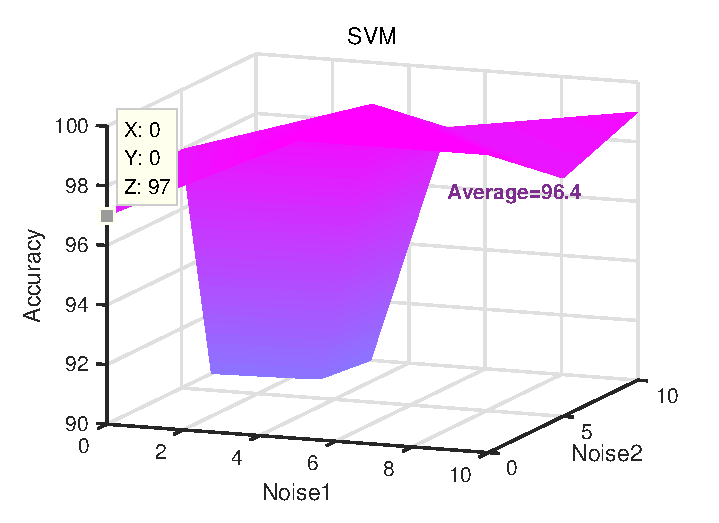
\includegraphics[width=4cm]{1-23.eps}
}
	\subfigure[imbalance ratio = 3]{
	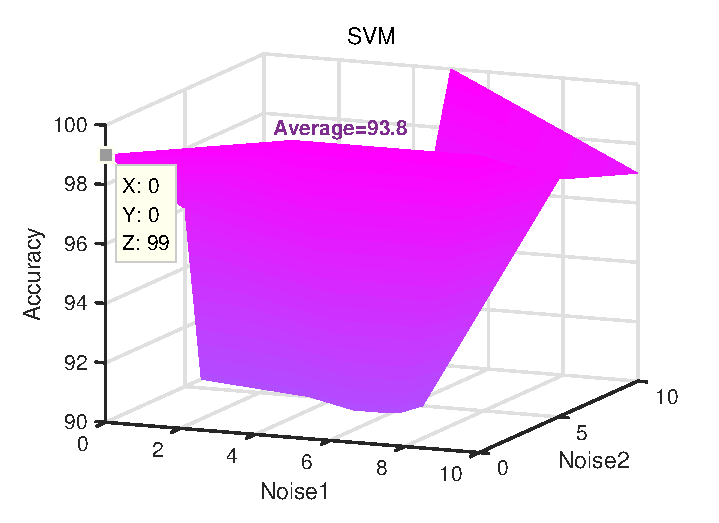
\includegraphics[width=4cm]{1-32.eps}
}
	\subfigure[imbalance ratio = 4]{
	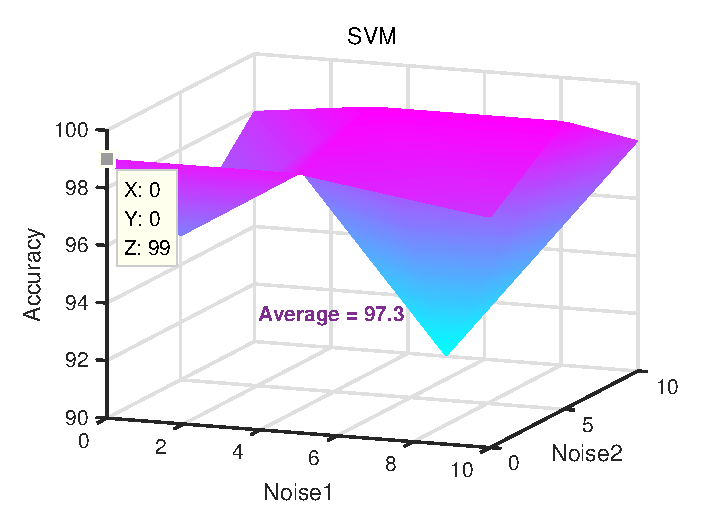
\includegraphics[width=4cm]{1-43.eps}
}
	\subfigure[imbalance ratio = 5]{
	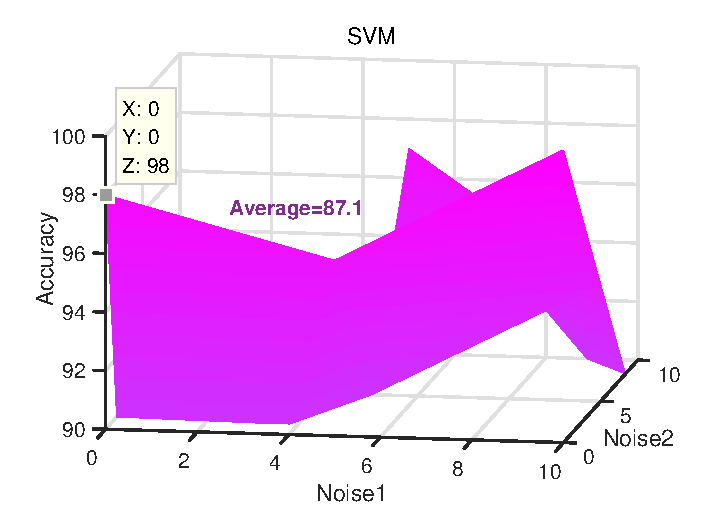
\includegraphics[width=4cm]{1-52.eps}
}
   	\subfigure[imbalance ratio = 2]{
	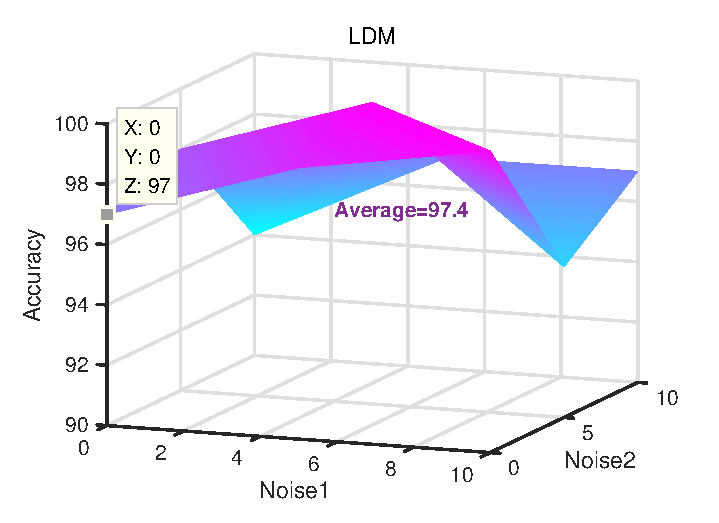
\includegraphics[width=4cm]{1-22.eps}
}
	\subfigure[imbalance ratio = 3]{
	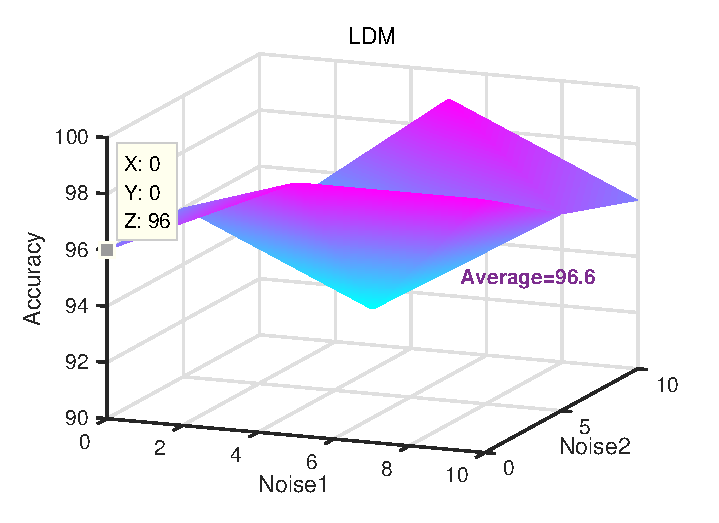
\includegraphics[width=4cm]{1-33.eps}
}
	\subfigure[imbalance ratio = 4]{
	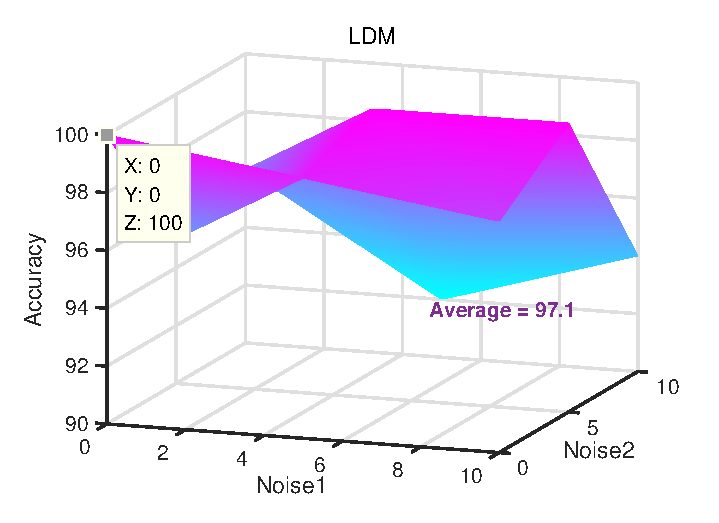
\includegraphics[width=4cm]{1-42.eps}
}
	\subfigure[imbalance ratio = 5]{
	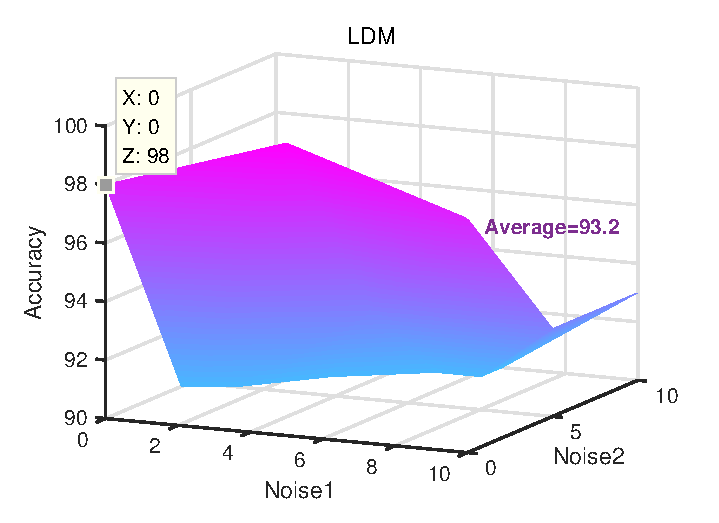
\includegraphics[width=4cm]{1-53.eps}
}
	\subfigure[imbalance ratio = 2]{
	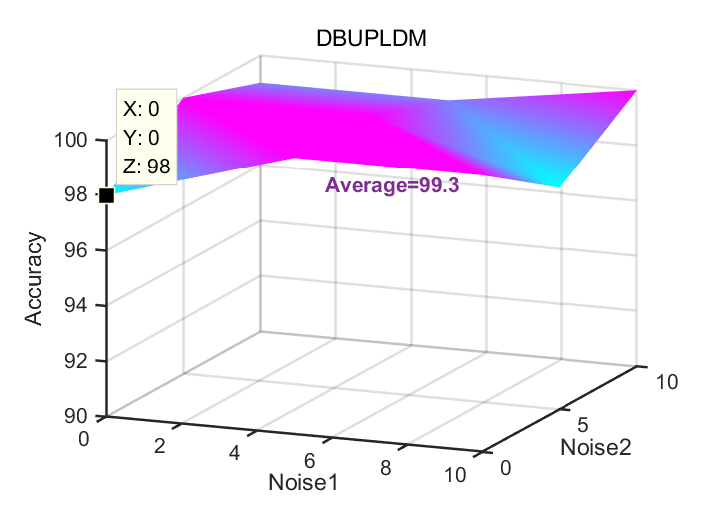
\includegraphics[width=4cm]{1-21.eps}
}
	\subfigure[imbalance ratio = 3]{
	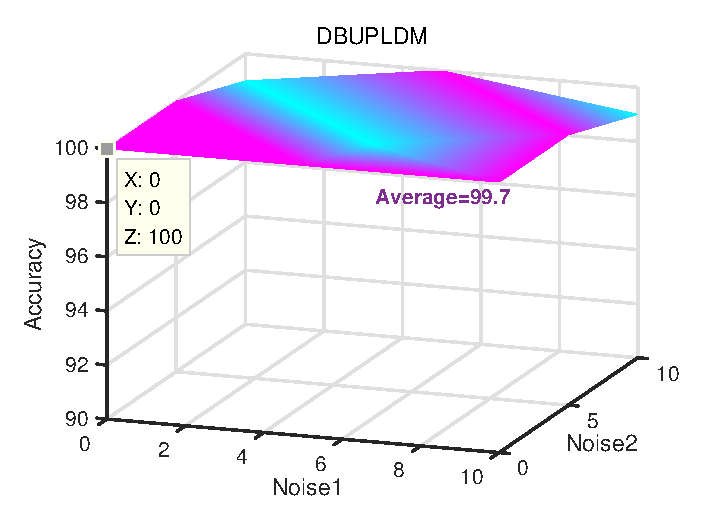
\includegraphics[width=4cm]{1-31.eps}
}
	\subfigure[imbalance ratio = 4]{
	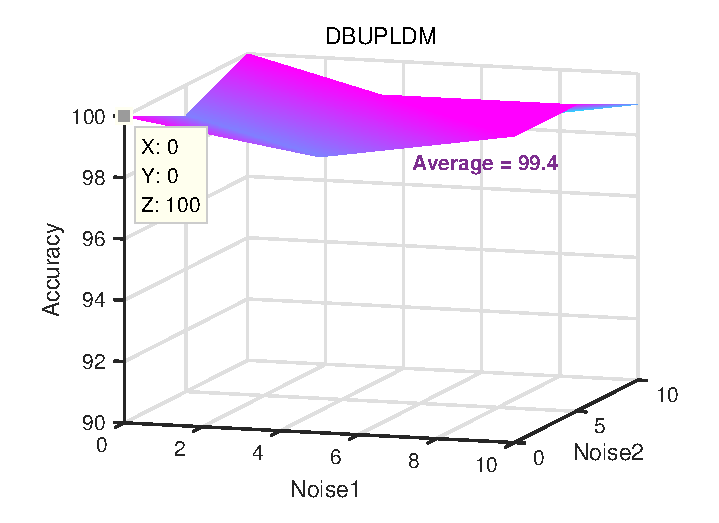
\includegraphics[width=4cm]{1-41.eps}
}
	\subfigure[imbalance ratio = 5]{
	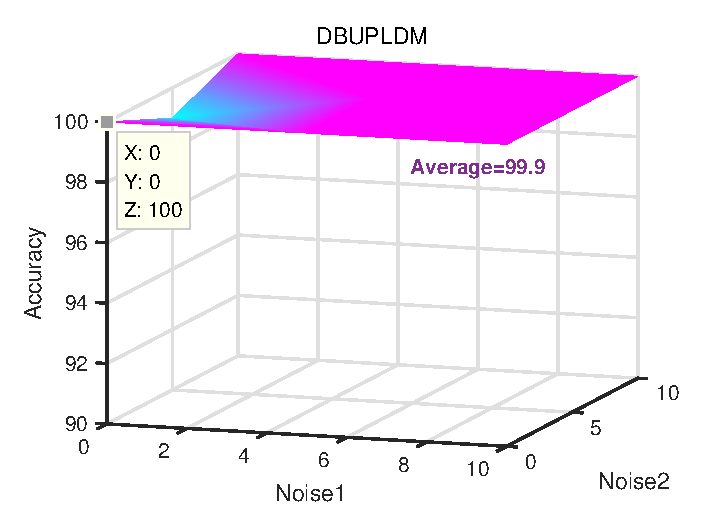
\includegraphics[width=4cm]{1-51.eps}
}
	\caption{ \color{blue}{Noise immunity performance of SVM, LDM, and DBUPLDM under the different imbalance ratios.}} 
	\label{Ir}
\end{figure*}



\begin{figure*}[h] 
	\centering %使插入的图片居中显示
	     % Give a unique label
	     \hspace{-19mm}
	\subfigure[$\tau=0$ with linear kernel (Accuracy=71.9\%)]{
	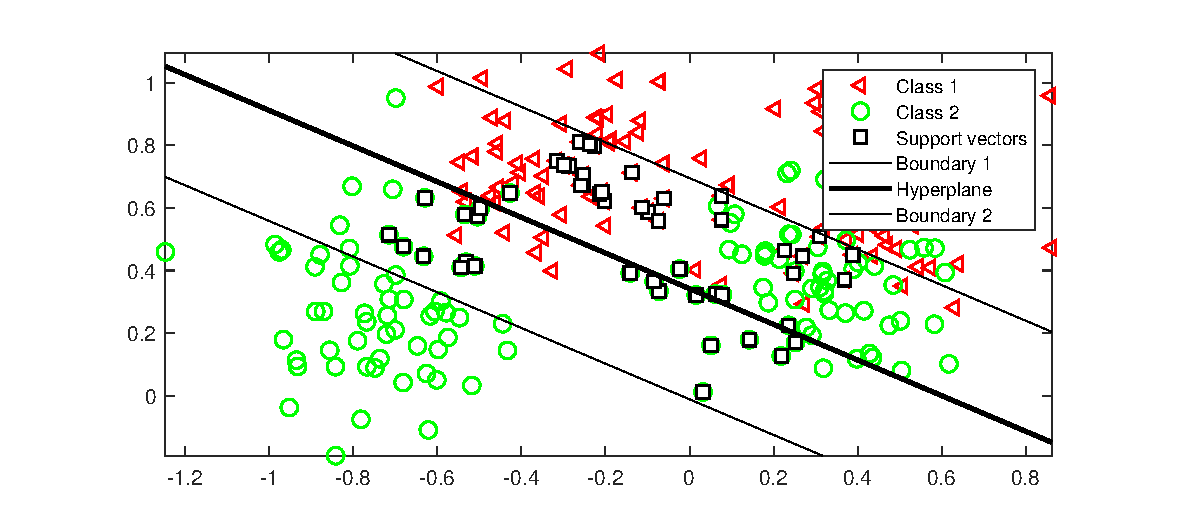
\includegraphics[width=8cm]{x1.eps}}\hspace{-7mm}
		\subfigure[$\tau=0$ with RBF kernel (Accuracy=90.7\%)]{
	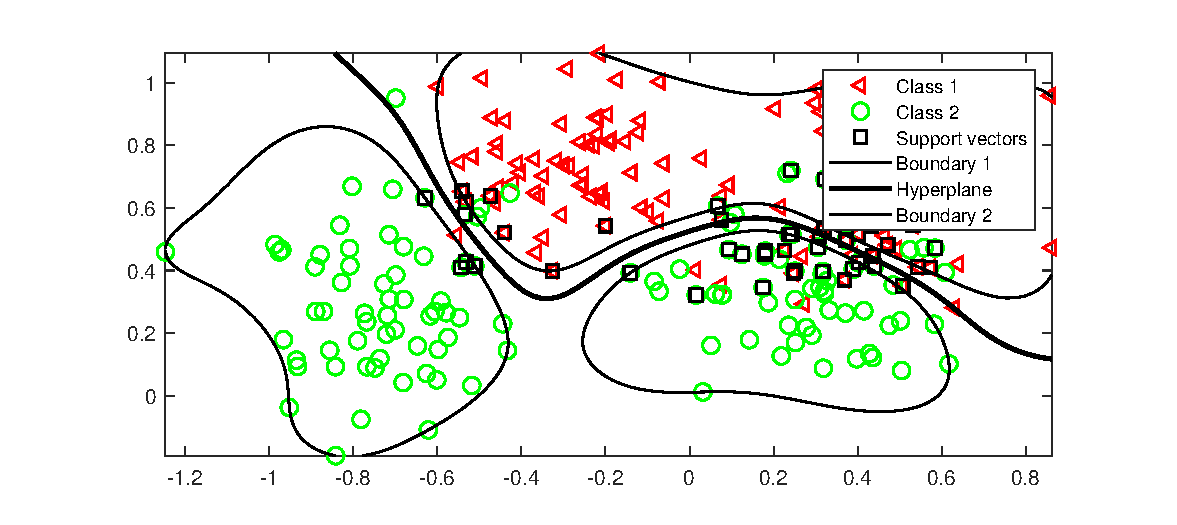
\includegraphics[width=8cm]{y1.eps}}\hspace{-14mm}
	
	\hspace{-18mm}
		\subfigure[$\tau=-0.3$ with linear kernel (Accuracy=72.0\%)]{
	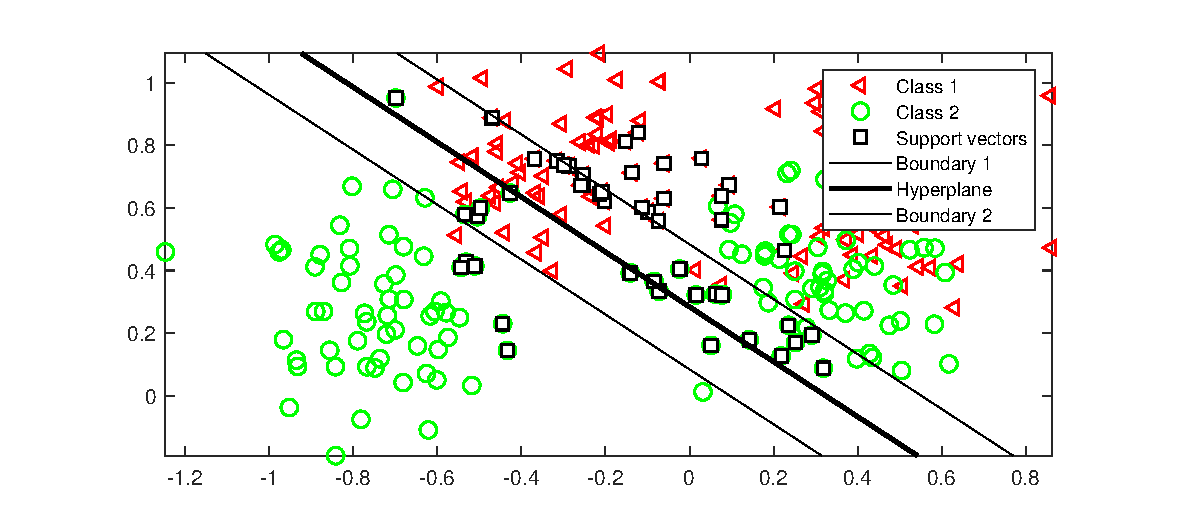
\includegraphics[width=8cm]{xx1.eps}}\hspace{-7mm}
		\subfigure[$\tau=0.3$ with RBF kernel (Accuracy=90.9\%)]{
	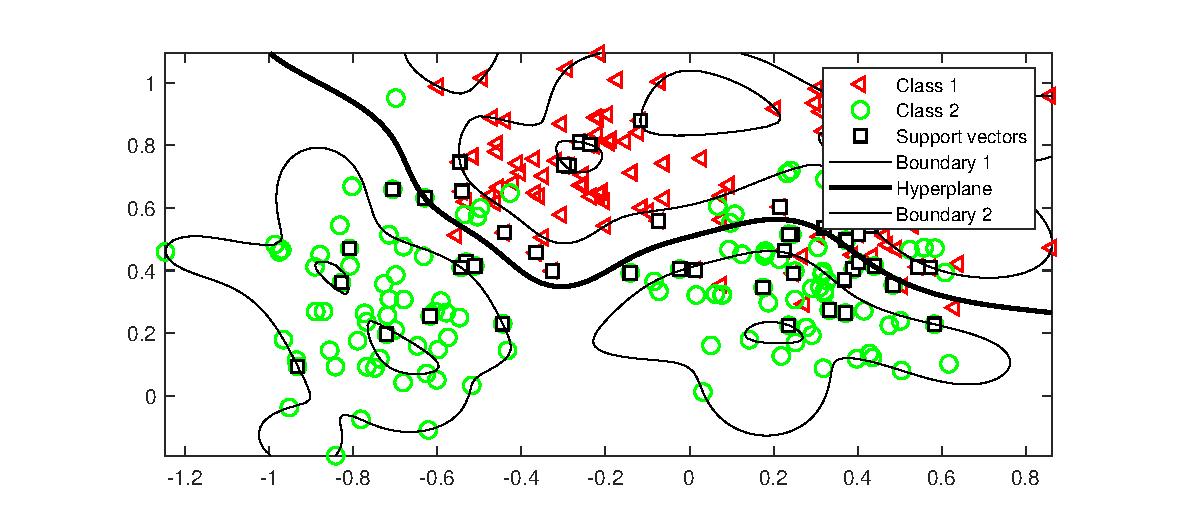
\includegraphics[width=8cm]{yy1.eps}} \hspace{-14mm}
	\caption{Comparison of classification accuracy corresponding to different $\tau$ values and kernel functions.}
	\label{fig3}  
\end{figure*}

\subsection{Parameter settings}\label{setting}
Data points in the datasets are normalized to $[0,1]$ to avoid the dominance of input features with greater numerical values over other smaller values. The traversal range of parameters in the experiment is $\eta \in [\{2^{-6},2^{-5},2^{-4}, \ldots, 2^1$, $2^2,2^3\}]$, $\sigma$ (parameter of Gaussian kernel) $\in \{2^{-7},2^{-6},...,2^{7}\}$, $\tau \in$\{-1,-0.99,-0.98,...,0,0.01,0.02,...,1\}, $\lambda_1$  $\in\{2^{-7},2^{-6},...,2^{1}\}$, $\lambda_2$ traverses the same range as $\lambda_1$. The accuracy of each algorithm depends on the optimal combination of these parameters. All experiments in this paper are performed on a computer with 8 × 4.00 GHz CPU and 32 GB of memory using MATLAB R2018a. 

\subsection{Experiments on artificial datasets}\label{5.1.1}

To verify the performance of DBUPLDM for the imbalance classification task, we conducted experiments using datasets with varying levels of imbalance and added different types of noise. Each sample or noise point $x_{i}$ follows a normal distribution, such that: ${x_i}$ $\sim$ $\mathcal{N}({\mathcal{\mu}},{\Sigma})$, where $\mathcal{\mu}$ and $\Sigma$ represent the mean and covariance of the two dimensions of the sample, respectively. The details of our experimental setup are summarized in Table \ref{aset}.


The imbalance ratio changes as the number of majority class samples is varied. To verify the anti-noise performance of DBUPLDM, the amount of noise in each category is controlled from 0 to 10, varying the degree of imbalance, and the experimental results are shown in Fig. \ref{Ir}.

Fig. \ref{Ir} compares the noise immunity performance of DBUPLDM with that of LDM and SVM on an imbalanced classification task. The three algorithms are evaluated using varying levels of positive class and negative class noise, and an imbalance ratio of 2, 3, 4, or 5. As shown in Fig. \ref{Ir}, DBUPLDM consistently achieves the highest accuracy when no noise is added, regardless of the imbalance ratio (as indicated in the figure caption). When a certain amount of noise is introduced, the classification accuracy curves for SVM and LDM fluctuate significantly, indicating their high sensitivity to noise. Compared to SVM, LDM has better noise immunity due to its consideration of marginal theory. However, the accuracy surface of DBUPLDM remains smoother while still achieving higher accuracy. Furthermore, as the imbalance ratio increases, the accuracy surfaces of SVM and LDM become more volatile due to the statistical characteristics of the data. On the other hand, DBUPLDM consistently maintains the highest average accuracy and stability despite varying degrees of imbalance. These experimental results effectively demonstrate the superior noise immunity and generalization performance of DBUPLDM.

To provide a more intuitive understanding of how DBUPLDM handles boundary points with varying $\tau$ values, we conduct experiments on the artificially synthesized two-dimensional dataset Ripley. Fig. \ref{fig3} presents the boundary information obtained from these experiments.

As illustrated by Fig. \ref{fig3}, in the case of a linear kernel, when $\tau=-0.3$, points located outside of the positive and negative hyperplanes receive a negative penalty, resulting in a decrease in the margin between the hyperplanes. Similarly, for a Gaussian kernel, when $\tau=0.3$, the margin between hyperplanes increases. The different $\tau$ values correspond to different quantile levels, demonstrating the flexibility of DBUPLDM.

When $\tau=0$, DBUPLDM degenerates into DBLDM with hinge loss, as shown in $(a)$ and $(b)$ of Fig. \ref{fig3}. By comparing the accuracy rates, it is clear that DBUPLDM achieves higher accuracy with different $\tau$ values, whether using a linear kernel or a Gaussian kernel. These experiments demonstrate that DBUPLDM has better flexibility and is less affected by boundary noise compared to traditional LDM.

%-------------TABLE 1--------------------------
\begin{table*}
\footnotesize
  \centering 
\caption{\color{orange}Comparison of Accuracy, AUC, and F1-score of SVM, PinSVM, UPSVM, LDM, and DBUPLDM on the UCI datasets}
\label{tabel1}
     \setlength{\tabcolsep}{1.5mm}{ % 微调列间距
    \resizebox{\textwidth}{!}{
            \begin{tabular}{cc cccc cccc ccccc ccccc ccccc}
    \toprule
    \multirow{2}{*}{$\eta$} & \multirow{2}{*}{Dataset} & \multicolumn{4}{c}{SVM} & \multicolumn{4}{c}{LDM} & \multicolumn{5}{c}{PinSVM} & \multicolumn{5}{c}{UPSVM} & \multicolumn{5}{c}{\textbf{DBUPLDM}} \\
\cmidrule{3-25}    & & Acc & {\color{orange}AUC} & {\color{orange}F1} & C & Acc & {\color{orange}AUC} & {\color{orange}F1} & C & Acc & {\color{orange}AUC} & {\color{orange}F1} & C & $\tau$ & Acc & {\color{orange}AUC} & {\color{orange}F1} & C & $\tau$ & Acc & {\color{orange}AUC} & {\color{orange}F1} & C & $\tau$ \\
    \midrule
    
\multirow{18}[4]{*}{$\eta$ = 1} & Monk1 & 64.35  & {\color{orange}62.54} & {\color{orange}0.65} & 0.06  & 67.59  & {\color{orange}68.22} & {\color{orange}0.70} & 0.06  & 65.28  & {\color{orange}65.15} & {\color{orange}0.68} & 0.03  & 0.20  & 66.44  & {\color{orange}66.30} & {\color{orange}0.69} & 4.00  & -0.40  & \textbf{68.29 } & \textbf{{\color{orange}72.55}} & \textbf{{\color{orange}0.75}} & 1.00  & 0.70  \\
          & Monk2 & 67.13  & {\color{orange}65.42} & {\color{orange}0.68} & 0.02  & 67.13  & {\color{orange}65.38} & {\color{orange}0.68} & 0.02  & 67.13  & {\color{orange}65.26} & {\color{orange}0.68} & 0.02  & -0.90  & 67.13  & {\color{orange}65.32} & {\color{orange}0.68} & 0.02  & -0.40  & \textbf{67.82 } & \textbf{{\color{orange}67.63}} & \textbf{{\color{orange}0.70}} & 0.50  & 0.50  \\
          & Monk3 & 81.02  & {\color{orange}79.18} & {\color{orange}0.81} & 0.06  & 84.03  & {\color{orange}83.45} & {\color{orange}0.85} & 0.13  & 84.26  & {\color{orange}83.32} & {\color{orange}0.85} & 0.02  & 1.00  & 86.34  & {\color{orange}85.67} & {\color{orange}0.87} & 0.25  & -0.40  & \textbf{88.89 } & \textbf{{\color{orange}89.21}} & \textbf{{\color{orange}0.91}} & 0.50  & -0.30  \\
          & Pima-Indian & 76.42  & {\color{orange}71.27} & {\color{orange}0.74} & 0.02  & 77.36  & {\color{orange}72.41} & {\color{orange}0.75} & 0.02  & 77.36  & {\color{orange}73.19} & {\color{orange}0.76} & 1.00  & -1.00  & 76.42  & {\color{orange}71.35} & {\color{orange}0.74} & 0.02  & -0.30  & \textbf{78.30}  & \textbf{{\color{orange}75.83}} & \textbf{{\color{orange}0.78}} & 2.00  & 0.50  \\
          & WDBC  & 86.67  & {\color{orange}85.23} & {\color{orange}0.87} & 0.06  & 85.00  & {\color{orange}84.17} & {\color{orange}0.86} & 0.06  & 86.67  & {\color{orange}85.31} & {\color{orange}0.87} & 0.06  & 0.00  & 86.67  & {\color{orange}85.29} & {\color{orange}0.87} & 0.06  & 0.00  & \textbf{87.50 } & \textbf{{\color{orange}87.66}} & \textbf{{\color{orange}0.89}} & 0.06  & 0.20  \\
          & Echo  & \textbf{94.04 } & \textbf{{\color{orange}92.45}} & \textbf{{\color{orange}0.93}} & 2.00  & 93.38  & {\color{orange}91.62} & {\color{orange}0.92} & 8.00  & \textbf{94.04 } & {\color{orange}92.38} & \textbf{{\color{orange}0.93}} & 2.00  & 0.00  & \textbf{94.04 } & {\color{orange}92.42} & {\color{orange}0.93} & 2.00  & 0.00  & 92.05  & {\color{orange}90.58} & {\color{orange}0.91} & 0.02  & -0.90  \\
          & Ionosphere & 67.09  & {\color{orange}65.78} & {\color{orange}0.68} & 0.02  & \textbf{79.91 } & \textbf{{\color{orange}78.55}} & \textbf{{\color{orange}0.80}} & 2.00  & 71.15  & {\color{orange}66.42} & {\color{orange}0.69} & 0.03  & -1.00  & 71.15  & {\color{orange}70.63} & {\color{orange}0.73} & 8.00  & -0.70  & 79.06  & {\color{orange}75.92} & {\color{orange}0.78} & 8.00  & -0.30  \\
          & Heberman & 79.29  & {\color{orange}78.63} & {\color{orange}0.80} & 0.02  & \textbf{98.82 } & {\color{orange}98.37} & {\color{orange}0.89} & 0.06  & 95.86  & {\color{orange}95.24} & {\color{orange}0.86} & 0.02  & 0.10  & 95.86  & {\color{orange}95.31} & {\color{orange}0.81} & 0.02  & 0.10  & \textbf{98.82 } & \textbf{{\color{orange}98.55} } & \textbf{{\color{orange}0.91}} & 0.50  & -0.20  \\
          & Statlog & 70.59  & {\color{orange}70.32} & {\color{orange}0.73} & 0.02  & 88.24  & {\color{orange}87.51} & {\color{orange}0.88} & 0.03  & 70.59  & {\color{orange}70.28} & {\color{orange}0.73} & 0.02  & 0.00  & 90.20  & {\color{orange}89.46} & {\color{orange}0.91} & 0.25  & -0.20  & \textbf{92.16 } & \textbf{{\color{orange}91.74}} & \textbf{{\color{orange}0.93}} & 0.25  & -0.50  \\
          & Germans & 32.80  & {\color{orange}30.55} & {\color{orange}0.33} & 0.02  & 68.00  & {\color{orange}67.36} & {\color{orange}0.69} & 0.02  & 67.20  & {\color{orange}65.82} & {\color{orange}0.67} & 0.25  & -1.00  & 67.20  & {\color{orange}65.74} & {\color{orange}0.67} & 8.00  & -0.80  & \textbf{76.20 } & \textbf{{\color{orange}75.69}} & \textbf{{\color{orange}0.77}} & 2.00  & -0.10  \\
          & Australian & 84.48  & {\color{orange}83.76} & {\color{orange}0.85} & 0.03  & 86.55  & {\color{orange}85.42} & {\color{orange}0.87} & 0.03  & 84.48  & {\color{orange}83.61} & {\color{orange}0.85} & 0.03  & 0.00  & \textbf{87.24 } & {\color{orange}86.58} & {\color{orange}0.88} & 0.03  & -0.30  & \textbf{87.24 } & \textbf{{\color{orange}87.82}} & \textbf{{\color{orange}0.89}} & 0.03  & -0.90  \\
          & Votes & 85.11  & {\color{orange}84.63} & {\color{orange}0.86} & 0.02  & \textbf{95.74}  & {\color{orange}95.28} & {\color{orange}0.96} & 1.00  & 94.04  & {\color{orange}94.15} & {\color{orange}0.95} & 0.02  & -0.90  & 91.49  & {\color{orange}91.37} & {\color{orange}0.93} & 0.02  & -0.10  & 95.32  & \textbf{{\color{orange}95.76}} & \textbf{{\color{orange}0.97}} & 0.50  & 0.00  \\
          & Diabetes & 67.91  & {\color{orange}66.41} & {\color{orange}0.69} & 0.02  & 81.72  & {\color{orange}80.57} & \textbf{{\color{orange}0.82}} & 1.00  & 67.91  & {\color{orange}66.38} & {\color{orange}0.69} & 0.02  & 0.00  & 72.76  & {\color{orange}71.45} & {\color{orange}0.73} & 8.00  & -0.80  & \textbf{81.72}  & \textbf{{\color{orange}80.83}} & \textbf{{\color{orange}0.82}} & 2.00  & -0.50  \\
          & Fertility & \textbf{94.00 } & {\color{orange}93.27} & {\color{orange}0.94} & 0.02  & \textbf{94.00 } & {\color{orange}93.31} & {\color{orange}0.94} & 0.02  & \textbf{94.00 } & {\color{orange}93.25} & {\color{orange}0.94} & 0.02  & 0.00  & \textbf{94.00 } & {\color{orange}93.30} & {\color{orange}0.94} & 0.02  & 0.00  & \textbf{94.00 } & \textbf{{\color{orange}94.66}} & \textbf{{\color{orange}0.95}} & 0.02  & -1.00  \\
          & Sonar & 69.44  & {\color{orange}68.55} & {\color{orange}0.71} & 0.13  & 74.07  & {\color{orange}73.62} & {\color{orange}0.76} & 0.06  & 72.22  & {\color{orange}70.89} & {\color{orange}0.73} & 0.02  & -1.00  & 74.07  & {\color{orange}73.58} & {\color{orange}0.76} & 0.03  & -0.30  & \textbf{76.85 } & \textbf{{\color{orange}75.74}} & \textbf{{\color{orange}0.78}} & 0.50  & 0.40  \\
          & Ecoil & 86.61  & {\color{orange}85.38} & {\color{orange}0.87} & 0.25  & \textbf{94.49 } & {\color{orange}94.23} & {\color{orange}0.87} & 0.13  & \textbf{94.49 } & {\color{orange}94.18} & {\color{orange}0.85} & 0.06  & 0.90  & \textbf{94.49 } & {\color{orange}94.21} & {\color{orange}0.86} & 0.25  & -0.10  & \textbf{94.49 } & \textbf{{\color{orange}94.77}} & \textbf{{\color{orange}0.91}} & 0.02  & -1.00  \\
          & Plrx  & 67.07  & {\color{orange}66.42} & {\color{orange}0.69} & 0.02  & 67.07  & {\color{orange}66.35} & {\color{orange}0.69} & 0.02  & 67.07  & {\color{orange}66.28} & {\color{orange}0.69} & 0.02  & 0.00  & 67.07  & {\color{orange}66.32} & {\color{orange}0.69} & 0.02  & -1.00  & \textbf{70.73 } & \textbf{{\color{orange}70.59}} & \textbf{{\color{orange}0.73}} & 2.00  & 0.40  \\
\cmidrule{2-25}          & \textbf{Ave. } & 74.94  & {\color{orange}70.42} & {\color{orange}0.73} &       & 82.50  & {\color{orange}76.38} & {\color{orange}0.79} &       & 79.63  & {\color{orange}74.26} & {\color{orange}0.77} &       &       & 81.33  & {\color{orange}75.41} & {\color{orange}0.78} &       &       & \textbf{84.08 } & \textbf{{\color{orange}80.68}} & \textbf{{\color{orange}0.83}} &       & \\
    \midrule
    \multirow{18}[4]{*}{$\eta$ = 0.5} & Monk1 & 62.73  & {\color{orange}62.35} & {\color{orange}0.65} & 0.13  & 67.59  & {\color{orange}68.22} & {\color{orange}0.70} & 0.06  & 65.28  & {\color{orange}65.15} & {\color{orange}0.68} & 0.03  & 0.20  & 66.44  & {\color{orange}66.30} & {\color{orange}0.69} & 4.00  & -0.40  & \textbf{68.29 } & \textbf{{\color{orange}72.55}}
     & \textbf{{\color{orange}0.75}} & 1.00  & 0.70  \\
          & Monk2 & 67.13  & {\color{orange}65.42} & \textbf{{\color{orange}0.68}} & 0.02  & 67.13  & {\color{orange}65.38} & \textbf{{\color{orange}0.68}} & 0.02  & 67.13  & {\color{orange}65.26} & \textbf{{\color{orange}0.68}} & 0.02  & -0.90  & 67.13  & {\color{orange}65.32} & \textbf{{\color{orange}0.68}} & 0.02  & -0.40  & \textbf{67.59 } & \textbf{{\color{orange}67.92}} & {\color{orange}0.67} & 0.50  & 0.90  \\
          & Monk3 & 81.02  & {\color{orange}79.18} & {\color{orange}0.81} & 0.06  & 84.03  & {\color{orange}83.45} & {\color{orange}0.85} & 0.13  & 84.26  & {\color{orange}83.32} & {\color{orange}0.85} & 0.02  & 1.00  & 86.34  & {\color{orange}85.67} & {\color{orange}0.87} & 0.25  & -0.40  & \textbf{88.89 } & \textbf{{\color{orange}89.21}} & \textbf{{\color{orange}0.91}} & 0.50  & -0.30  \\
          & Pima-Indian & 76.42  & {\color{orange}71.27} & {\color{orange}0.74} & 0.02  & 77.36  & {\color{orange}72.41} & {\color{orange}0.75} & 0.02  & 78.30  & {\color{orange}73.19} & {\color{orange}0.76} & 0.25  & -1.00  & 76.42  & {\color{orange}71.35} & {\color{orange}0.74} & 0.02  & -0.30  & \textbf{79.25 } & \textbf{{\color{orange}76.75}} & \textbf{{\color{orange}0.79}} & 4.00  & 0.30  \\
          & WDBC  & 86.67  & {\color{orange}85.23} & {\color{orange}0.87} & 0.06  & 85.00  & {\color{orange}84.17} & {\color{orange}0.86} & 0.06  & 86.67  & {\color{orange}85.31} & {\color{orange}0.87} & 0.06  & 0.00  & 86.67  & {\color{orange}85.29} & {\color{orange}0.87} & 0.06  & 0.00  & \textbf{87.50 } & \textbf{{\color{orange}87.66}} & \textbf{{\color{orange}0.89}} & 0.06  & 0.20  \\
          & Echo  & \textbf{94.04 } & \textbf{{\color{orange}92.45}} & \textbf{{\color{orange}0.93}} & 2.00  & 93.38  & {\color{orange}91.62} & {\color{orange}0.92} & 8.00  & \textbf{94.04 } & {\color{orange}92.38} & \textbf{{\color{orange}0.93}} & 2.00  & 0.00  & \textbf{94.04 } & {\color{orange}92.42} & \textbf{{\color{orange}0.93}} & 2.00  & 0.00  & 92.72  & {\color{orange}90.87} & {\color{orange}0.91} & 2.00  & 1.00  \\
          & Ionosphere & 67.09  & {\color{orange}65.78} & {\color{orange}0.68} & 0.02  & \textbf{79.91 } & \textbf{{\color{orange}78.55}} & \textbf{{\color{orange}0.80}} & 2.00  & 67.95  & {\color{orange}66.42} & {\color{orange}0.69} & 0.06  & -1.00  & 71.15  & {\color{orange}70.63} & {\color{orange}0.73} & 8.00  & -0.70  & 78.42  & {\color{orange}75.63} & {\color{orange}0.78} & 8.00  & 0.20  \\
          & Heberman & 79.29  & {\color{orange}78.63} & {\color{orange}0.80} & 0.02  & \textbf{98.82 } & {\color{orange}91.37} & {\color{orange}0.89} & 0.06  & 95.86  & {\color{orange}95.24} & {\color{orange}0.86} & 0.02  & 0.10  & 95.86  & {\color{orange}90.31} & {\color{orange}0.85} & 0.02  & 0.10  & \textbf{98.82 } & \textbf{{\color{orange}91.55}} & \textbf{{\color{orange}0.92}} & 0.50  & -0.20  \\
          & Statlog & 70.59  & {\color{orange}70.32} & {\color{orange}0.73} & 0.02  & 88.24  & {\color{orange}87.51} & {\color{orange}0.88} & 0.03  & 76.47  & {\color{orange}75.28} & {\color{orange}0.78} & 4.00  & -1.00  & 90.20  & {\color{orange}89.46} & {\color{orange}0.91} & 0.25  & -0.20  & \textbf{92.16 } & \textbf{{\color{orange}91.74}} & \textbf{{\color{orange}0.93}} & 0.13  & -0.50  \\
          & Germans & 32.80  & {\color{orange}30.55} & {\color{orange}0.33} & 0.02  & 68.00  & {\color{orange}67.36} & {\color{orange}0.69} & 0.02  & 67.20  & {\color{orange}65.82} & {\color{orange}0.67} & 0.06  & -1.00  & 67.20  & {\color{orange}65.74} & {\color{orange}0.67} & 2.00  & -0.80  & \textbf{77.40 } & \textbf{{\color{orange}75.92}} & \textbf{{\color{orange}0.77}} & 8.00  & -0.60  \\
          & Australian & 84.48  & {\color{orange}83.76} & {\color{orange}0.85} & 0.03  & 86.55  & {\color{orange}85.42} & {\color{orange}0.87} & 0.03  & 84.48  & {\color{orange}83.61} & {\color{orange}0.85} & 0.03  & 0.00  & \textbf{87.24 } & {\color{orange}86.58} & {\color{orange}0.88} & 0.03  & -0.30  & \textbf{87.24 } & \textbf{{\color{orange}87.82}} & \textbf{{\color{orange}0.89}} & 0.03  & -0.90  \\
          & Votes & 85.11  & {\color{orange}84.63} & {\color{orange}0.86} & 0.02  & \textbf{95.74 } & {\color{orange}95.28} & {\color{orange}0.87} & 1.00  & 94.04  & {\color{orange}94.15} & {\color{orange}0.83} & 0.02  & -0.90  & 91.49  & {\color{orange}91.37} & {\color{orange}0.89} & 0.02  & -0.10  & 94.89  & \textbf{{\color{orange}95.42}} & \textbf{{\color{orange}0.90}} & 0.25  & -0.50  \\
          & Diabetes & 67.91  & {\color{orange}66.41} & {\color{orange}0.69} & 0.02  & \textbf{81.72}  & {\color{orange}80.57} & {\color{orange}0.82} & 1.00  & 72.76  & {\color{orange}71.45} & {\color{orange}0.73} & 0.25  & -1.00  & 72.76  & {\color{orange}71.45} & {\color{orange}0.73} & 8.00  & -0.80  & \textbf{81.72}  & \textbf{{\color{orange}80.95}} & \textbf{{\color{orange}0.82}} & 0.25  & -0.60  \\
          & Fertility & \textbf{94.00 } & {\color{orange}93.27} & {\color{orange}0.94} & 0.02  & \textbf{94.00 } & {\color{orange}93.31} & {\color{orange}0.94} & 0.02  & \textbf{94.00 } & {\color{orange}93.25} & {\color{orange}0.94} & 0.02  & 0.00  & \textbf{94.00 } & {\color{orange}93.30} & {\color{orange}0.94} & 0.02  & 0.00  & \textbf{94.00 } & \textbf{{\color{orange}94.82}} & \textbf{{\color{orange}0.95}} & 0.02  & -1.00  \\
          & Sonar & 69.44  & {\color{orange}68.55} & {\color{orange}0.71} & 0.13  & 74.07  & {\color{orange}73.62} & {\color{orange}0.76} & 0.06  & 71.30  & {\color{orange}70.67} & {\color{orange}0.73} & 0.06  & 0.10  & 74.07  & {\color{orange}73.58} & {\color{orange}0.76} & 0.03  & -0.30  & \textbf{76.85 } & \textbf{{\color{orange}75.91}} & \textbf{{\color{orange}0.78}} & 0.50  & 0.40  \\
          & Ecoil & 86.61  & {\color{orange}85.38} & {\color{orange}0.87} & 0.25  & \textbf{94.49 } & {\color{orange}94.23} & {\color{orange}0.85} & 0.13  & \textbf{94.49 } & {\color{orange}94.18} & {\color{orange}0.81} & 0.06  & 0.90  & \textbf{94.49 } & {\color{orange}94.21} & {\color{orange}0.80} & 0.25  & -0.10  & \textbf{94.49 } & \textbf{{\color{orange}94.93}} & \textbf{{\color{orange}0.88}} & 0.02  & -1.00  \\
          & Plrx  & 67.07  & {\color{orange}66.42} & {\color{orange}0.69} & 0.02  & 67.07  & {\color{orange}66.35} & {\color{orange}0.69} & 0.02  & \textbf{68.29 } & {\color{orange}67.55} & {\color{orange}0.69} & 0.02  & -1.00  & 67.07  & {\color{orange}66.32} & {\color{orange}0.69} & 0.02  & -1.00  & \textbf{68.29 } & \textbf{{\color{orange}69.78}} & \textbf{{\color{orange}0.73}} & 8.00  & -0.20  \\
\cmidrule{2-25}          & \textbf{Ave. } & 74.85  & {\color{orange}71.36} & {\color{orange}0.74} &       & 82.50  & {\color{orange}77.25} & {\color{orange}0.80} &       & 82.54  & {\color{orange}75.42} & {\color{orange}0.78} &       &       & 80.15  & {\color{orange}76.38} & {\color{orange}0.79} &       &       & \textbf{84.03 } & \textbf{{\color{orange}81.55}} & \textbf{{\color{orange}0.84}} &       &  \\
    \midrule
    \multirow{18}[3]{*}{$\eta$ = 0.25} & Monk1 & 62.73  & {\color{orange}62.35} & {\color{orange}0.65} & 0.13  & 67.59  & {\color{orange}68.22} & {\color{orange}0.70} & 0.06  & 65.28  & {\color{orange}65.15} & {\color{orange}0.68} & 0.03  & 0.20  & 66.44  & {\color{orange}66.30} & {\color{orange}0.69} & 4.00  & -0.40  & \textbf{68.29 } & \textbf{{\color{orange}72.55}} & \textbf{{\color{orange}0.75}} & 1.00  & 0.70  \\
          & Monk2 & 67.13  & {\color{orange}65.42} & {\color{orange}0.68} & 0.02  & 67.13  & {\color{orange}65.38} & {\color{orange}0.68} & 0.02  & 67.13  & {\color{orange}65.26} & {\color{orange}0.68} & 0.02  & -0.90  & 67.13  & {\color{orange}65.32} & {\color{orange}0.68} & 0.02  & -0.40  & \textbf{68.29 } & \textbf{{\color{orange}66.87}} & \textbf{{\color{orange}0.69}} & 1.00  & 0.10  \\
          & Monk3 & 81.02  & {\color{orange}79.18} & {\color{orange}0.81} & 0.06  & 84.03  & {\color{orange}83.45} & {\color{orange}0.85} & 0.13  & 84.26  & {\color{orange}83.32} & {\color{orange}0.85} & 0.02  & 1.00  & 86.34  & {\color{orange}85.67} & {\color{orange}0.87} & 0.25  & -0.40  & \textbf{88.89 } & \textbf{{\color{orange}89.21}} & \textbf{{\color{orange}0.91}} & 0.50  & -0.30  \\
          & Pima-Indian & 76.42  & {\color{orange}71.27} & {\color{orange}0.74} & 0.02  & 77.36  & {\color{orange}72.41} & {\color{orange}0.75} & 0.02  & 78.30  & {\color{orange}73.19} & {\color{orange}0.76} & 0.25  & -1.00  & 76.42  & {\color{orange}71.35} & {\color{orange}0.74} & 0.02  & -0.30  & \textbf{79.25 } & \textbf{{\color{orange}76.42}} & \textbf{{\color{orange}0.79}} & 8.00  & 0.10  \\
          & WDBC  & 86.67  & {\color{orange}85.23} & {\color{orange}0.87} & 0.06  & 85.00  & {\color{orange}84.17} & {\color{orange}0.86} & 0.06  & 86.67  & {\color{orange}85.31} & {\color{orange}0.87} & 0.06  & 0.00  & 86.67  & {\color{orange}85.29} & {\color{orange}0.87} & 0.06  & 0.00  & \textbf{87.50 } & \textbf{{\color{orange}87.66}} & \textbf{{\color{orange}0.89}} & 0.06  & 0.20  \\
          & Echo  & \textbf{94.04 } & \textbf{{\color{orange}92.45}} & \textbf{{\color{orange}0.89}} & 2.00  & 93.38  & {\color{orange}91.62} & {\color{orange}0.92} & 8.00  & \textbf{94.04 } & {\color{orange}92.38} & {\color{orange}0.83} & 2.00  & 0.00  & \textbf{94.04 } & {\color{orange}92.42} & {\color{orange}0.81} & 2.00  & 0.00  & 92.72  & {\color{orange}90.87} & {\color{orange}0.81} & 8.00  & -0.30  \\
          & Ionosphere & 67.09  & {\color{orange}65.78} & {\color{orange}0.68} & 0.02  & \textbf{79.91 } & \textbf{{\color{orange}78.55}} & \textbf{{\color{orange}0.80}} & 2.00  & 67.95  & {\color{orange}66.42} & {\color{orange}0.69} & 0.06  & -1.00  & 71.15  & {\color{orange}70.63} & {\color{orange}0.73} & 8.00  & -0.70  & 79.06  & {\color{orange}75.63} & {\color{orange}0.78} & 2.00  & 0.40  \\
          & Heberman & 79.29  & {\color{orange}78.63} & {\color{orange}0.80} & 0.02  & \textbf{98.82 } & {\color{orange}98.37} & {\color{orange}0.89} & 0.06  & 95.86  & {\color{orange}95.24} & {\color{orange}0.86} & 0.02  & 0.10  & 95.86  & {\color{orange}95.31} & {\color{orange}0.86} & 0.02  & 0.10  & \textbf{98.82 } & \textbf{{\color{orange}98.55}} & \textbf{{\color{orange}0.90}} & 0.50  & -0.20  \\
          & Statlog & 70.59  & {\color{orange}70.32} & {\color{orange}0.73} & 0.02  & 88.24  & {\color{orange}87.51} & {\color{orange}0.88} & 0.03  & 76.47  & {\color{orange}75.28} & {\color{orange}0.78} & 4.00  & -1.00  & 90.20  & {\color{orange}89.46} & {\color{orange}0.91} & 0.25  & -0.20  & \textbf{92.16 } & \textbf{{\color{orange}91.74}} & \textbf{{\color{orange}0.93}} & 0.25  & -0.50  \\
          & Germans & 32.80  & {\color{orange}30.55} & {\color{orange}0.33} & 0.02  & 68.00  & {\color{orange}67.36} & {\color{orange}0.69} & 0.02  & 67.20  & {\color{orange}65.82} & {\color{orange}0.67} & 0.06  & -1.00  & 67.20  & {\color{orange}65.74} & {\color{orange}0.67} & 2.00  & -0.80  & \textbf{76.80 } & \textbf{{\color{orange}75.92}} & \textbf{{\color{orange}0.77}} & 4.00  & 0.40  \\
          & Australian & 84.48  & {\color{orange}83.76} & {\color{orange}0.85} & 0.03  & 86.55  & {\color{orange}85.42} & {\color{orange}0.87} & 0.03  & 84.48  & {\color{orange}83.61} & {\color{orange}0.85} & 0.03  & 0.00  & \textbf{87.24 } & {\color{orange}86.58} & {\color{orange}0.88} & 0.03  & -0.30  & \textbf{87.24 } & \textbf{{\color{orange}87.82}} & \textbf{{\color{orange}0.89}} & 0.03  & -0.90  \\
          & Votes & 85.11  & {\color{orange}84.63} & {\color{orange}0.86} & 0.02  & 95.74  & {\color{orange}95.28} & {\color{orange}0.96} & 1.00  & 94.04  & {\color{orange}94.15} & {\color{orange}0.95} & 0.02  & -0.90  & 91.49  & {\color{orange}91.37} & {\color{orange}0.93} & 0.02  & -0.10  & \textbf{96.17 } & \textbf{{\color{orange}95.42}} & \textbf{{\color{orange}0.97}} & 1.00  & 0.70  \\
          & Diabetes & 67.91  & {\color{orange}66.41} & {\color{orange}0.69} & 0.02  & 81.72  & {\color{orange}80.57} & {\color{orange}0.82} & 1.00  & 72.76  & {\color{orange}71.45} & {\color{orange}0.73} & 0.25  & -1.00  & 72.76  & {\color{orange}71.45} & {\color{orange}0.73} & 8.00  & -0.80  & \textbf{82.09}  & \textbf{{\color{orange}80.95}} & \textbf{{\color{orange}0.82}} & 0.25  & -0.60  \\
          & Fertility & \textbf{94.00 } & {\color{orange}93.27} & {\color{orange}0.94} & 0.02  & \textbf{94.00 } & {\color{orange}93.31} & {\color{orange}0.94} & 0.02  & \textbf{94.00 } & {\color{orange}93.25} & {\color{orange}0.94} & 0.02  & 0.00  & \textbf{94.00 } & {\color{orange}93.30} & {\color{orange}0.94} & 0.02  & 0.00  & \textbf{94.00 } & \textbf{{\color{orange}94.82}} & \textbf{{\color{orange}0.95}} & 0.02  & -1.00  \\
          & Sonar & 69.44  & {\color{orange}68.55} & {\color{orange}0.71} & 0.13  & 74.07  & {\color{orange}73.62} & {\color{orange}0.76} & 0.06  & 71.30  & {\color{orange}70.67} & {\color{orange}0.73} & 0.06  & 0.10  & 74.07  & {\color{orange}73.58} & {\color{orange}0.76} & 0.03  & -0.30  & \textbf{76.85 } & \textbf{{\color{orange}75.91}} & \textbf{{\color{orange}0.78}} & 0.50  & 0.40  \\
          & Ecoil & 86.61  & {\color{orange}85.38} & {\color{orange}0.87} & 0.25  & \textbf{94.49 } & {\color{orange}94.23} & {\color{orange}0.95} & 0.13  & \textbf{94.49 } & {\color{orange}94.18} & {\color{orange}0.95} & 0.06  & 0.90  & \textbf{94.49 } & {\color{orange}94.21} & {\color{orange}0.95} & 0.25  & -0.10  & \textbf{94.49 } & \textbf{{\color{orange}94.93}} & \textbf{{\color{orange}0.96}} & 0.02  & -1.00  \\
          & Plrx  & 67.07  & {\color{orange}66.42} & {\color{orange}0.69} & 0.02  & 67.07  & {\color{orange}66.35} & {\color{orange}0.69} & 0.02  & 68.29  & {\color{orange}67.55} & {\color{orange}0.69} & 0.02  & -1.00  & 67.07  & {\color{orange}66.32} & {\color{orange}0.69} & 0.02  & -1.00  & \textbf{69.51 } & \textbf{{\color{orange}69.78}} & \textbf{{\color{orange}0.73}} & 8.00  & -0.10  \\
\cmidrule{2-25}          & \textbf{Ave. } & 74.85  & {\color{orange}71.36} & {\color{orange}0.74} &       & 82.54  & {\color{orange}77.63} & {\color{orange}0.80} &       & 80.15  & {\color{orange}75.87} & {\color{orange}0.78} &       &       & 81.33  & {\color{orange}76.82} & {\color{orange}0.79} &       &       & \textbf{84.24 } & \textbf{{\color{orange}81.83}} & \textbf{{\color{orange}0.84}} &       &  \\
\midrule
    \end{tabular}}}
    \label{uci1}
\end{table*}



% %-------------TABLE 2--------------------------
% \begin{table*}
% \footnotesize
%   \centering 
% \caption{\color{orange}Comparison of Accuracy, AUC, and F1-score of SVM, PinSVM, UPSVM, LDM, and DBUPLDM on the UCI datasets}
% \label{uci2}
%      \setlength{\tabcolsep}{1.5mm}{ % 微调列间距
%     \resizebox{\textwidth}{!}{
%             \begin{tabular}{cc cccc cccc ccccc ccccc ccccc}
%     \toprule
%     \multirow{2}{*}{$\eta$} & \multirow{2}{*}{Dataset} & \multicolumn{4}{c}{SVM} & \multicolumn{4}{c}{LDM} & \multicolumn{5}{c}{PinSVM} & \multicolumn{5}{c}{UPSVM} & \multicolumn{5}{c}{\textbf{DBUPLDM}} \\
% \cmidrule{3-22}    & & Acc & {\color{orange}AUC} & {\color{orange}F1} & C & Acc & {\color{orange}AUC} & {\color{orange}F1} & C & Acc & {\color{orange}AUC} & {\color{orange}F1} & C & $\tau$ & Acc & {\color{orange}AUC} & {\color{orange}F1} & C & $\tau$ & Acc & {\color{orange}AUC} & {\color{orange}F1} & C & $\tau$ \\

%     \midrule
% \multirow{17}[4]{*}{$\eta$ = 0.125} 
% & Monk1 & 62.73 & \color{orange}61.50 & \color{orange}0.63 & 0.13 & 67.59 & \color{orange}66.80 & \color{orange}0.69 & 0.06 & 65.28 & \color{orange}64.30 & \color{orange}0.66 & 0.03 & 0.20 & 66.44 & \color{orange}65.10 & \color{orange}0.67 & 4.00 & -0.40 & \textbf{68.29} & \textbf{\color{orange}72.55} & \textbf{\color{orange}0.75} & 1.00 & 0.70 \\
% & Monk2 & 67.13 & \color{orange}65.42 & \color{orange}0.68 & 0.02 & 67.13 & \color{orange}65.38 & \color{orange}0.68 & 0.02 & 67.13 & \color{orange}65.26 & \color{orange}0.68 & 0.02 & -0.90 & 67.13 & \color{orange}65.32 & \color{orange}0.68 & 0.02 & -0.40 & \textbf{67.82} & \textbf{\color{orange}66.87} & \textbf{\color{orange}0.69} & 8.00 & -0.20 \\
% & Monk3 & 81.02 & \color{orange}79.18 & \color{orange}0.81 & 0.06 & 84.03 & \color{orange}83.45 & \color{orange}0.85 & 0.13 & 84.26 & \color{orange}83.32 & \color{orange}0.85 & 0.02 & 1.00 & 86.34 & \color{orange}85.67 & \color{orange}0.87 & 0.25 & -0.40 & \textbf{88.89} & \textbf{\color{orange}89.21} & \textbf{\color{orange}0.91} & 0.50 & -0.30 \\
% & Pima-Indian & 76.42 & \color{orange}71.27 & \color{orange}0.74 & 0.02 & 77.36 & \color{orange}72.41 & \color{orange}0.75 & 0.02 & 78.30 & \color{orange}73.19 & \color{orange}0.76 & 0.25 & -1.00 & 76.42 & \color{orange}71.35 & \color{orange}0.74 & 0.02 & -0.30 & \textbf{79.25} & \textbf{\color{orange}75.83} & \textbf{\color{orange}0.78} & 8.00 & 0.20 \\
% & WDBC & 86.67 & \color{orange}85.23 & \color{orange}0.87 & 0.06 & 85.00 & \color{orange}84.17 & \color{orange}0.86 & 0.06 & 86.67 & \color{orange}85.31 & \color{orange}0.87 & 0.06 & 0.00 & 86.67 & \color{orange}85.29 & \color{orange}0.87 & 0.06 & 0.00 & \textbf{87.50} & \textbf{\color{orange}87.66} & \textbf{\color{orange}0.89} & 0.06 & 0.20 \\
% & Echo & \textbf{94.04} & \textbf{\color{orange}92.45} & \textbf{\color{orange}0.93} & 2.00 & 93.38 & \color{orange}91.62 & \color{orange}0.92 & 8.00 & \textbf{94.04} & \textbf{\color{orange}92.38} & \textbf{\color{orange}0.93} & 2.00 & 0.00 & \textbf{94.04} & \textbf{\color{orange}92.42} & \textbf{\color{orange}0.93} & 2.00 & 0.00 & 92.72 & \color{orange}90.58 & \color{orange}0.91 & 4.00 & 0.70 \\
% & Ionosphere & 67.09 & \color{orange}65.78 & \color{orange}0.68 & 0.02 & \textbf{79.91} & \textbf{\color{orange}78.55} & \textbf{\color{orange}0.80} & 2.00 & 67.95 & \color{orange}66.42 & \color{orange}0.69 & 0.06 & -1.00 & 71.15 & \color{orange}70.63 & \color{orange}0.73 & 8.00 & -0.70 & 78.85 & \color{orange}75.92 & \color{orange}0.78 & 2.00 & 0.40 \\
% & Heberman & 79.29 & \color{orange}78.63 & \color{orange}0.80 & 0.02 & \textbf{98.82} & \textbf{\color{orange}98.37} & \textbf{\color{orange}0.99} & 0.06 & 95.86 & \color{orange}95.24 & \color{orange}0.96 & 0.02 & 0.10 & 95.86 & \color{orange}95.31 & \color{orange}0.96 & 0.02 & 0.10 & \textbf{98.82} & \textbf{\color{orange}98.55} & \textbf{\color{orange}0.99} & 0.50 & -0.20 \\
% & Statlog & 70.59 & \color{orange}70.32 & \color{orange}0.73 & 0.02 & 88.24 & \color{orange}87.51 & \color{orange}0.88 & 0.03 & 70.59 & \color{orange}70.28 & \color{orange}0.73 & 0.02 & 0.00 & 90.20 & \color{orange}89.46 & \color{orange}0.91 & 0.25 & -0.20 & \textbf{92.16} & \textbf{\color{orange}91.74} & \textbf{\color{orange}0.93} & 0.25 & -0.50 \\
% & Germans & 32.80 & \color{orange}30.55 & \color{orange}0.33 & 0.02 & 68.00 & \color{orange}67.36 & \color{orange}0.69 & 0.02 & 67.20 & \color{orange}65.82 & \color{orange}0.67 & 0.25 & -1.00 & 67.20 & \color{orange}65.74 & \color{orange}0.67 & 8.00 & -0.80 & \textbf{76.20} & \textbf{\color{orange}75.69} & \textbf{\color{orange}0.77} & 2.00 & -0.10 \\
% & Australian & 84.48 & \color{orange}83.76 & \color{orange}0.85 & 0.03 & 86.55 & \color{orange}85.42 & \color{orange}0.87 & 0.03 & 84.48 & \color{orange}83.61 & \color{orange}0.85 & 0.03 & 0.00 & \textbf{87.24} & \textbf{\color{orange}86.58} & \textbf{\color{orange}0.88} & 0.03 & -0.30 & \textbf{87.24} & \textbf{\color{orange}87.82} & \textbf{\color{orange}0.89} & 0.03 & -0.90 \\
% & Votes & 85.11 & \color{orange}84.63 & \color{orange}0.86 & 0.02 & \textbf{95.74} & \textbf{\color{orange}95.28} & \textbf{\color{orange}0.96} & 1.00 & 94.04 & \color{orange}94.15 & \color{orange}0.95 & 0.02 & -0.90 & 91.49 & \color{orange}91.37 & \color{orange}0.93 & 0.02 & -0.10 & 95.32 & \color{orange}95.76 & \color{orange}0.97 & 0.50 & 0.00 \\
% & Diabetes & 67.91 & \color{orange}66.41 & \color{orange}0.69 & 0.02 & \textbf{81.72} & \textbf{\color{orange}80.57} & \textbf{\color{orange}0.82} & 1.00 & 67.91 & \color{orange}66.38 & \color{orange}0.69 & 0.02 & 0.00 & 72.76 & \color{orange}71.45 & \color{orange}0.73 & 8.00 & -0.80 & 81.72 & \color{orange}80.83 & \color{orange}0.82 & 2.00 & -0.50 \\
% & Fertility & \textbf{94.00} & \textbf{\color{orange}93.27} & \textbf{\color{orange}0.94} & 0.02 & \textbf{94.00} & \textbf{\color{orange}93.31} & \textbf{\color{orange}0.94} & 0.02 & \textbf{94.00} & \textbf{\color{orange}93.25} & \textbf{\color{orange}0.94} & 0.02 & 0.00 & \textbf{94.00} & \textbf{\color{orange}93.30} & \textbf{\color{orange}0.94} & 0.02 & 0.00 & \textbf{94.00} & \textbf{\color{orange}94.66} & \textbf{\color{orange}0.95} & 0.02 & -1.00 \\
% & Sonar & 69.44 & \color{orange}68.55 & \color{orange}0.71 & 0.13 & 74.07 & \color{orange}73.62 & \color{orange}0.76 & 0.06 & 72.22 & \color{orange}70.89 & \color{orange}0.73 & 0.02 & -1.00 & 74.07 & \color{orange}73.58 & \color{orange}0.76 & 0.03 & -0.30 & \textbf{76.85} & \textbf{\color{orange}75.74} & \textbf{\color{orange}0.78} & 0.50 & 0.40 \\
% & Ecoil & 86.61 & \color{orange}85.38 & \color{orange}0.87 & 0.25 & \textbf{94.49} & \textbf{\color{orange}94.23} & \textbf{\color{orange}0.95} & 0.13 & \textbf{94.49} & \textbf{\color{orange}94.18} & \textbf{\color{orange}0.95} & 0.06 & 0.90 & \textbf{94.49} & \textbf{\color{orange}94.21} & \textbf{\color{orange}0.95} & 0.25 & -0.10 & \textbf{94.49} & \textbf{\color{orange}94.77} & \textbf{\color{orange}0.96} & 0.02 & -1.00 \\
% & Plrx & 67.07 & \color{orange}66.42 & \color{orange}0.69 & 0.02 & 67.07 & \color{orange}66.35 & \color{orange}0.69 & 0.02 & 67.07 & \color{orange}66.28 & \color{orange}0.69 & 0.02 & 0.00 & 67.07 & \color{orange}66.32 & \color{orange}0.69 & 0.02 & -1.00 & \textbf{70.73} & \textbf{\color{orange}70.59} & \textbf{\color{orange}0.73} & 2.00 & 0.40 \\
% \cmidrule{2-25}
% & \textbf{Ave.} & 74.73 & {\color{orange}71.58} & {\color{orange}0.75} & & 82.59 & {\color{orange}78.00} & {\color{orange}0.76} & & 80.15 & {\color{orange}76.15} & {\color{orange}0.76} & & & 81.33 & {\color{orange}76.30} & {\color{orange}0.76} & & & \textbf{84.25} & \textbf{\color{orange}82.53} & \textbf{\color{orange}0.84} & & \\

% \midrule

% \multirow{17}[4]{*}{$\eta$ = 0.0625} 
% & Monk1 & 62.73 & \color{orange}61.35 & \color{orange}0.62 & 0.13 & 67.59 & \color{orange}66.60 & \color{orange}0.68 & 0.06 & 65.28 & \color{orange}64.10 & \color{orange}0.65 & 0.03 & 0.20 & 66.44 & \color{orange}65.00 & \color{orange}0.66 & 4.00 & -0.40 & \textbf{68.29} & \textbf{\color{orange}72.45} & \textbf{\color{orange}0.74} & 1.00 & 0.70 \\
% & Monk2 & 67.13 & \color{orange}65.32 & \color{orange}0.67 & 0.02 & 67.13 & \color{orange}65.28 & \color{orange}0.67 & 0.02 & 67.13 & \color{orange}65.16 & \color{orange}0.67 & 0.02 & -0.90 & 67.13 & \color{orange}65.22 & \color{orange}0.67 & 0.02 & -0.40 & \textbf{67.59} & \textbf{\color{orange}66.77} & \textbf{\color{orange}0.68} & 8.00 & -0.20 \\
% & Monk3 & 81.02 & \color{orange}79.08 & \color{orange}0.80 & 0.06 & 84.03 & \color{orange}83.35 & \color{orange}0.84 & 0.13 & 84.26 & \color{orange}83.22 & \color{orange}0.84 & 0.02 & 1.00 & 86.34 & \color{orange}85.57 & \color{orange}0.86 & 0.25 & -0.40 & \textbf{88.89} & \textbf{\color{orange}89.11} & \textbf{\color{orange}0.90} & 0.50 & -0.30 \\
% & Pima-Indian & 76.42 & \color{orange}71.17 & \color{orange}0.73 & 0.02 & 77.36 & \color{orange}72.31 & \color{orange}0.74 & 0.02 & 78.30 & \color{orange}73.09 & \color{orange}0.75 & 0.25 & -1.00 & 76.42 & \color{orange}71.25 & \color{orange}0.73 & 0.02 & -0.30 & \textbf{79.25} & \textbf{\color{orange}75.73} & \textbf{\color{orange}0.77} & 8.00 & 0.20 \\
% & WDBC & 86.67 & \color{orange}85.13 & \color{orange}0.86 & 0.06 & 85.00 & \color{orange}84.07 & \color{orange}0.85 & 0.06 & 86.67 & \color{orange}85.21 & \color{orange}0.86 & 0.06 & 0.00 & 86.67 & \color{orange}85.19 & \color{orange}0.86 & 0.06 & 0.00 & \textbf{87.50} & \textbf{\color{orange}87.56} & \textbf{\color{orange}0.88} & 0.06 & 0.20 \\
% & Echo & \textbf{94.04} & \textbf{\color{orange}92.35} & \textbf{\color{orange}0.92} & 2.00 & 93.38 & \color{orange}91.52 & \color{orange}0.91 & 8.00 & \textbf{94.04} & \color{orange}92.28 & \textbf{\color{orange}0.92} & 2.00 & 0.00 & \textbf{\color{black}94.04} & \color{orange}92.32 & \textbf{\color{orange}0.92} & 2.00 & 0.00 & 92.62 & \color{orange}90.48 & \color{orange}0.90 & 4.00 & 0.70 \\
% & Ionosphere & 67.09 & \color{orange}65.68 & \color{orange}0.67 & 0.02 & \textbf{79.81} & \textbf{\color{orange}78.45} & \textbf{\color{orange}0.79} & 2.00 & 67.95 & \color{orange}66.32 & \color{orange}0.68 & 0.06 & -1.00 & 71.15 & \color{orange}70.53 & \color{orange}0.72 & 8.00 & -0.70 & 78.75 & \color{orange}75.82 & \color{orange}0.77 & 2.00 & 0.40 \\
% & Heberman & 79.29 & \color{orange}78.53 & \color{orange}0.79 & 0.02 & \textbf{98.72} & \color{orange}94.14 & \color{orange}0.88 & 0.06 & 95.86 & \color{orange}95.14 & \color{orange}0.85 & 0.02 & 0.10 & 95.86 & \color{orange}95.21 & \color{orange}0.85 & 0.02 & 0.10 & \textbf{98.72} & \textbf{\color{orange}94.45} & \textbf{\color{orange}0.89} & 0.50 & -0.20 \\
% & Statlog & 70.59 & \color{orange}70.22 & \color{orange}0.72 & 0.02 & 88.24 & \color{orange}87.41 & \color{orange}0.87 & 0.03 & 70.59 & \color{orange}70.18 & \color{orange}0.72 & 0.02 & 0.00 & 90.20 & \color{orange}89.36 & \color{orange}0.90 & 0.25 & -0.20 & \textbf{92.16} & \textbf{\color{orange}91.64} & \textbf{\color{orange}0.92} & 0.25 & -0.50 \\
% & Germans & 32.80 & \color{orange}30.45 & \color{orange}0.32 & 0.02 & 68.00 & \color{orange}67.26 & \color{orange}0.68 & 0.02 & 67.20 & \color{orange}65.72 & \color{orange}0.66 & 0.25 & -1.00 & 67.20 & \color{orange}65.64 & \color{orange}0.66 & 8.00 & -0.80 & \textbf{76.20} & \textbf{\color{orange}75.59} & \textbf{\color{orange}0.76} & 2.00 & -0.10 \\
% & Australian & 84.48 & \color{orange}83.66 & \color{orange}0.84 & 0.03 & 86.55 & \color{orange}85.32 & \color{orange}0.86 & 0.03 & 84.48 & \color{orange}83.51 & \color{orange}0.84 & 0.03 & 0.00 & \textbf{87.14} & \color{orange}86.48 & \color{orange}0.87 & 0.03 & -0.30 & \textbf{87.14} & \textbf{\color{orange}87.72} & \textbf{\color{orange}0.88} & 0.03 & -0.90 \\
% & Votes & 85.11 & \color{orange}84.53 & \color{orange}0.85 & 0.02 & \textbf{95.64} & \color{orange}95.18 & \color{orange}0.85 & 1.00 & 94.04 & \color{orange}94.05 & \color{orange}0.84 & 0.02 & -0.90 & 91.49 & \color{orange}91.27 & \color{orange}0.82 & 0.02 & -0.10 & 95.22 & \color{orange}95.66 & \textbf{\color{orange}0.89} & 0.50 & 0.00 \\
% & Diabetes & 67.91 & \color{orange}66.31 & \color{orange}0.68 & 0.02 & \textbf{81.62} & \color{orange}80.47 & \textbf{\color{orange}0.81} & 1.00 & 67.91 & \color{orange}66.28 & \color{orange}0.68 & 0.02 & 0.00 & 72.76 & \color{orange}71.35 & \color{orange}0.72 & 8.00 & -0.80 & \textbf{81.62} & \textbf{\color{orange}80.73} & \textbf{\color{orange}0.81} & 2.00 & -0.50 \\
% & Fertility & \textbf{94.00} & \textbf{\color{orange}93.17} & \textbf{\color{orange}0.93} & 0.02 & \textbf{94.00} & \textbf{\color{orange}93.21} & \textbf{\color{orange}0.93} & 0.02 & \textbf{94.00} & \textbf{\color{orange}93.15} & \textbf{\color{orange}0.93} & 0.02 & 0.00 & \textbf{94.00} & \color{orange}93.20 & \color{orange}0.93 & 0.02 & 0.00 & \textbf{94.00} & \color{orange}94.56 & \color{orange}0.94 & 0.02 & -1.00 \\
% & Sonar & 69.44 & \color{orange}68.45 & \color{orange}0.70 & 0.13 & 74.07 & \color{orange}73.52 & \color{orange}0.75 & 0.06 & 72.22 & \color{orange}70.79 & \color{orange}0.72 & 0.02 & -1.00 & 74.07 & \color{orange}73.48 & \color{orange}0.75 & 0.03 & -0.30 & \textbf{76.85} & \textbf{\color{orange}75.64} & \textbf{\color{orange}0.77} & 0.50 & 0.40 \\
% & Ecoil & 86.61 & \color{orange}85.28 & \color{orange}0.86 & 0.25 & \textbf{94.49} & \color{orange}94.13 & \color{orange}0.84 & 0.13 & \textbf{94.49} & \color{orange}91.08 & \color{orange}0.84 & 0.06 & 0.90 & \textbf{94.49} & \color{orange}94.11 & \color{orange}0.94 & 0.25 & -0.10 & \textbf{94.90} & \textbf{\color{orange}94.67} & \textbf{\color{orange}0.89} & 0.02 & -1.00 \\
% & Plrx & 67.07 & \color{orange}66.32 & \color{orange}0.68 & 0.02 & 67.07 & \color{orange}66.25 & \color{orange}0.68 & 0.02 & 67.07 & \color{orange}66.18 & \color{orange}0.68 & 0.02 & 0.00 & 67.07 & \color{orange}66.22 & \color{orange}0.68 & 0.02 & -1.00 & \textbf{\color{orange}69.51} & \textbf{\color{orange}70.49} & \textbf{\color{orange}0.72} & 2.00 & 0.40 \\
% \cmidrule{2-25}
% & \textbf{Ave.} & 74.73 & \color{orange}71.07 & \color{orange}0.75 & & 82.59 & \color{orange}77.07 & \color{orange}0.76 & & 80.15 & \color{orange}75.17 & \color{orange}0.77 & & & 81.33 & \color{orange}76.27 & \color{orange}0.76 & & & \textbf{84.21} & \textbf{\color{orange}81.83} & \textbf{\color{orange}0.84} & & \\

% \midrule

% \multirow{18}[3]{*}{$\eta$ = 0.03125} 
% & Monk1 & 62.73 & \color{orange}62.21 & \color{orange}0.64 & 0.13 & 67.59 & \color{orange}68.05 & \color{orange}0.69 & 0.06 & 65.28 & \color{orange}65.30 & \color{orange}0.67 & 0.03 & 0.20 & 66.44 & \color{orange}66.12 & \color{orange}0.70 & 4.00 & -0.40 & \textbf{68.29} & \textbf{\color{orange}72.38} & \textbf{\color{orange}0.74} & 1.00 & 0.70 \\
% & Monk2 & 67.13 & \color{orange}65.58 & \color{orange}0.69 & 0.02 & 67.13 & \color{orange}65.21 & \color{orange}0.67 & 0.02 & 67.13 & \color{orange}65.41 & \color{orange}0.69 & 0.02 & -0.90 & 67.13 & \color{orange}65.47 & \color{orange}0.67 & 0.02 & -0.40 & \textbf{68.29} & \textbf{\color{orange}66.72} & \textbf{\color{orange}0.70} & 1.00 & 0.10 \\
% & Monk3 & 81.02 & \color{orange}79.33 & \color{orange}0.80 & 0.06 & 84.03 & \color{orange}83.59 & \color{orange}0.84 & 0.13 & 84.26 & \color{orange}83.17 & \color{orange}0.86 & 0.02 & 1.00 & 86.34 & \color{orange}85.82 & \color{orange}0.86 & 0.25 & -0.40 & \textbf{88.89} & \textbf{\color{orange}89.05} & \textbf{\color{orange}0.92} & 0.50 & -0.30 \\
% & Pima-Indian & 76.42 & \color{orange}71.41 & \color{orange}0.73 & 0.02 & 77.36 & \color{orange}72.56 & \color{orange}0.74 & 0.02 & 78.30 & \color{orange}73.04 & \color{orange}0.77 & 0.25 & -1.00 & 76.42 & \color{orange}71.50 & \color{orange}0.73 & 0.02 & -0.30 & \textbf{79.25} & \textbf{\color{orange}76.27} & \textbf{\color{orange}0.80} & 8.00 & 0.20 \\
% & WDBC & 86.67 & \color{orange}85.37 & \color{orange}0.86 & 0.06 & 85.00 & \color{orange}84.02 & \color{orange}0.87 & 0.06 & 86.67 & \color{orange}85.46 & \color{orange}0.86 & 0.06 & 0.00 & 86.67 & \color{orange}85.14 & \color{orange}0.88 & 0.06 & 0.00 & \textbf{87.50} & \textbf{\color{orange}87.81} & \textbf{\color{orange}0.88} & 0.06 & 0.20 \\
% & Echo & \textbf{\color{black}94.04} & \textbf{\color{orange}92.31} & \textbf{\color{orange}0.94} & 2.00 & 93.38 & \color{orange}91.77 & \color{orange}0.91 & 8.00 & \textbf{94.04} & \textbf{\color{orange}92.52} & \textbf{\color{orange}0.92} & 2.00 & 0.00 & \textbf{\color{black}94.04} & \textbf{\color{orange}92.28} & \textbf{\color{orange}0.94} & 2.00 & 0.00 & 92.72 & \color{orange}90.72 & \color{orange}0.92 & 8.00 & -0.30 \\
% & Ionosphere & 67.09 & \color{orange}65.63 & \color{orange}0.69 & 0.02 & \textbf{79.91} & \textbf{\color{orange}78.70} & \textbf{\color{orange}0.79} & 2.00 & 67.95 & \color{orange}66.57 & \color{orange}0.68 & 0.06 & -1.00 & 71.15 & \color{orange}70.48 & \color{orange}0.74 & 8.00 & -0.70 & 79.06 & \color{orange}76.07 & \color{orange}0.77 & 2.00 & 0.40 \\
% & Heberman & 79.29 & \color{orange}78.77 & \color{orange}0.79 & 0.02 & \textbf{98.82} & \textbf{\color{orange}98.22} & \textbf{\color{orange}1.00} & 0.06 & 95.86 & \color{orange}95.39 & \color{orange}0.95 & 0.02 & 0.10 & 95.86 & \color{orange}95.16 & \color{orange}0.97 & 0.02 & 0.10 & \textbf{98.82} & \textbf{\color{orange}98.40} & \textbf{\color{orange}0.98} & 0.50 & -0.20 \\
% & Statlog & 70.59 & \color{orange}70.47 & \color{orange}0.72 & 0.02 & 88.24 & \color{orange}87.36 & \color{orange}0.89 & 0.03 & 76.47 & \color{orange}75.41 & \color{orange}0.76 & 4.00 & -1.00 & 90.20 & \color{orange}89.31 & \color{orange}0.92 & 0.25 & -0.20 & \textbf{92.16} & \textbf{\color{orange}91.89} & \textbf{\color{orange}0.92} & 0.25 & -0.50 \\
% & Germans & 32.80 & \color{orange}30.40 & \color{orange}0.34 & 0.02 & 68.00 & \color{orange}67.51 & \color{orange}0.68 & 0.02 & 67.20 & \color{orange}65.67 & \color{orange}0.68 & 0.06 & -1.00 & 67.20 & \color{orange}65.89 & \color{orange}0.66 & 2.00 & -0.80 & \textbf{76.80} & \textbf{\color{orange}76.07} & \textbf{\color{orange}0.76} & 4.00 & 0.40 \\
% & Australian & 84.48 & \color{orange}83.61 & \color{orange}0.86 & 0.03 & 86.55 & \color{orange}85.57 & \color{orange}0.86 & 0.03 & 84.48 & \color{orange}83.76 & \color{orange}0.84 & 0.03 & 0.00 & \textbf{87.24} & \textbf{\color{orange}86.43} & \textbf{\color{orange}0.89} & 0.03 & -0.30 & \textbf{87.24} & \textbf{\color{orange}87.67} & \textbf{\color{orange}0.90} & 0.03 & -0.90 \\
% & Votes & 85.11 & \color{orange}84.78 & \color{orange}0.85 & 0.02 & \textbf{95.74} & \textbf{\color{orange}95.13} & \textbf{\color{orange}0.97} & 1.00 & 94.04 & \color{orange}94.30 & \color{orange}0.94 & 0.02 & -0.90 & 91.49 & \color{orange}91.22 & \color{orange}0.94 & 0.02 & -0.10 & \textbf{96.17} & \textbf{\color{orange}95.57} & \textbf{\color{orange}0.96} & 1.00 & 0.70 \\
% & Diabetes & 67.91 & \color{orange}66.56 & \color{orange}0.68 & 0.02 & \textbf{81.72} & \textbf{\color{orange}80.42} & \textbf{\color{orange}0.83} & 1.00 & 72.76 & \color{orange}71.70 & \color{orange}0.75 & 0.25 & -1.00 & 72.76 & \color{orange}71.60 & \color{orange}0.72 & 8.00 & -0.80 & 82.09 & \color{orange}81.10 & \color{orange}0.81 & 0.25 & -0.60 \\
% & Fertility & \textbf{94.00} & \textbf{\color{orange}93.41} & \textbf{\color{orange}0.93} & 0.02 & \textbf{94.00} & \textbf{\color{orange}93.16} & \textbf{\color{orange}0.95} & 0.02 & \textbf{94.00} & \textbf{\color{orange}93.40} & \textbf{\color{orange}0.93} & 0.02 & 0.00 & \textbf{94.00} & \textbf{\color{orange}93.15} & \textbf{\color{orange}0.95} & 0.02 & 0.00 & \textbf{94.00} & \textbf{\color{orange}94.51} & \textbf{\color{orange}0.94} & 0.02 & -1.00 \\
% & Sonar & 69.44 & \color{orange}68.40 & \color{orange}0.72 & 0.13 & 74.07 & \color{orange}73.77 & \color{orange}0.75 & 0.06 & 71.30 & \color{orange}70.50 & \color{orange}0.73 & 0.06 & 0.10 & 74.07 & \color{orange}73.73 & \color{orange}0.75 & 0.03 & -0.30 & \textbf{76.85} & \textbf{\color{orange}75.89} & \textbf{\color{orange}0.77} & 0.50 & 0.40 \\
% & Ecoil & 86.61 & \color{orange}85.53 & \color{orange}0.86 & 0.25 & \textbf{94.49} & \textbf{\color{orange}94.08} & \textbf{\color{orange}0.96} & 0.13 & \textbf{94.49} & \textbf{\color{orange}94.33} & \textbf{\color{orange}0.94} & 0.06 & 0.90 & \textbf{94.49} & \textbf{\color{orange}94.06} & \textbf{\color{orange}0.96} & 0.25 & -0.10 & \textbf{94.49} & \textbf{\color{orange}94.78} & \textbf{\color{orange}0.97} & 0.02 & -1.00 \\
% & Plrx & 67.07 & \color{orange}66.57 & \color{orange}0.68 & 0.02 & 67.07 & \color{orange}66.50 & \color{orange}0.68 & 0.02 & \textbf{68.29} & \textbf{\color{orange}67.10} & \textbf{\color{orange}0.71} & 0.02 & -1.00 & 67.07 & \color{orange}66.47 & \color{orange}0.68 & 0.02 & -1.00 & \textbf{69.51} & \textbf{\color{orange}69.63} & \textbf{\color{orange}0.73} & 8.00 & -0.10 \\
% \cmidrule{2-25}
% & \textbf{Ave.} & 74.85 & \color{orange}70.21 & \color{orange}0.74 & & 82.54 & \color{orange}76.94 & \color{orange}0.76 & & 80.15 & \color{orange}75.15 & \color{orange}0.77 & & & 81.33 & \color{orange}77.30 & \color{orange}0.76 & & & \textbf{84.01} & \textbf{\color{orange}81.34} & \textbf{\color{orange}0.84} & & \\
% \midrule
% & \textbf{Total Average} & 74.86 & \color{orange}71.06 & \color{orange}0.74 &  & 82.68 & \color{orange}77.75 & \color{orange}0.79 &  & 80.06 & \color{orange}75.35 & \color{orange}0.77 &  &  & 81.33 & \color{orange}76.06 & \color{orange}0.78 &  &  & \textbf{84.14} & \textbf{\color{orange}81.13} & \textbf{\color{orange}0.84} & &  \\
% \midrule
%     \end{tabular}}}
%     \label{uci2}
% \end{table*}

\begin{table*}[htbp] 
\renewcommand\arraystretch{1}
  \centering
  \footnotesize
  \caption{The number of wins, draws and losses for SVM, LDM, PinSVM, UPSVM and DBUPLDM}
  \setlength{\tabcolsep}{3mm}{
    \begin{tabular}{ccccccc}
    \toprule
          & $\eta$     & SVM   & UPSVM & PinSVM & \textbf{DBUPLDM} & LDM \\
    \midrule
    \multicolumn{1}{c}{\multirow{7}[4]{*}{\textbf{WIN}(Aggregated 17 datasets)}} & 1.00  & 3(68)     & 23(68)    & 14(68)    & \textbf{52(68)$\bullet$}    & 31(68) \\
          & 0.50  & 3(68)     & 23(68)    & 21(68)    & \textbf{51(68)$\bullet$}    & 31(68) \\
          & 0.25  & 3(68)     & 36(68)    & 21(68)    & \textbf{54(68)$\bullet$}    & 29(68) \\
          & 0.13  & 3(68)     & 22(68)    & 21(68)    & \textbf{57(68)$\bullet$}    & 31(68) \\
          & 0.06  & 3(68)     & 23(68)    & 20(68)    & \textbf{57(68)$\bullet$}    & 30(68) \\
          & 0.03  & 4(68)     & 24(68)    & 21(68)    & \textbf{53(68)$\bullet$}    & 31(68) \\
\cmidrule{2-7}          & ALL   & 19    & 151   & 118   & \textbf{324$\bullet$ } & 183  \\
    \midrule
    \multicolumn{1}{c}{\multirow{7}[4]{*}{\textbf{DRAW}\newline{}(Aggregated \newline{}17 datasets)}} & 1.00  & 18(68)    & 23(68)    & 24(68)    & 9(68)     & 14(68) \\
          & 0.50  & 15(68)    & 21(68)    & 19(68)    & 10(68)    & 13(68) \\
          & 0.25  & 15(68)    & 22(68)    & 18(68)    & 9(68)     & 11(68) \\
          & 0.13  & 14(68)    & 21(68)    & 17(68)    & 5(68)     & 13(68) \\
          & 0.06  & 14(68)    & 21(68)    & 17(68)    & 6(68)     & 14(68) \\
          & 0.03  & 15(68)    & 21(68)    & 19(68)    & 10(68)    & 14(68) \\
\cmidrule{2-7}          & ALL   & 91    & 129   & 114   & 49    & 79 \\
    \midrule
    \multicolumn{1}{c}{\multirow{7}[4]{*}{\textbf{LOSS}\newline{}(Aggregated \newline{}17 datasets)}} & 1.00  & 47(68)    & 22(68)    & 30(68)    & \textbf{7(68)$\circ$}     & 23(68) \\
          & 0.50  & 50(68)    & 24(68)    & 28(68)    & \textbf{7(68)$\circ$}      & 24(68) \\
          & 0.25  & 50(68)    & 10(68)    & 29(68)    & \textbf{5(68)$\circ$}     & 28(68) \\
          & 0.13  & 51(68)    & 25(68)    & 30(68)    & \textbf{6(68)$\circ$}    & 24(68) \\
          & 0.06  & 51(68)    & 24(68)    & 31(68)    & \textbf{5(68)$\circ$}     & 24(68) \\
          & 0.03  & 49(68)    & 23(68)    & 28(68)    & \textbf{5(68)$\circ$}     & 23(68) \\
\cmidrule{2-7}          & ALL   & 298   & 128   & 176   & \textbf{35$\circ$} & 146 \\
    \bottomrule
    \end{tabular}}%
    \label{win}
\end{table*}%




\begin{table*}[htbp]
  \centering
  \footnotesize
  \caption{Minimum distance with second order statistics}
  \vspace{2mm}
  \setlength{\tabcolsep}{8mm}{
    \begin{tabular}{lll}
    \toprule
        Method  & Hinge loss & Unified Pinball loss \\
    \midrule
    No Balanced Factors & 82.54 (LDM) & 83.54 (UPLDM) \\
    Balanced Factors & 83.02 (DBLDM) & \textbf{84.25 (DBUPLDM)} \\
    \bottomrule
    \end{tabular}}%
  \label{ab}%
\end{table*}%



\begin{figure*}[h] 
    \centering
    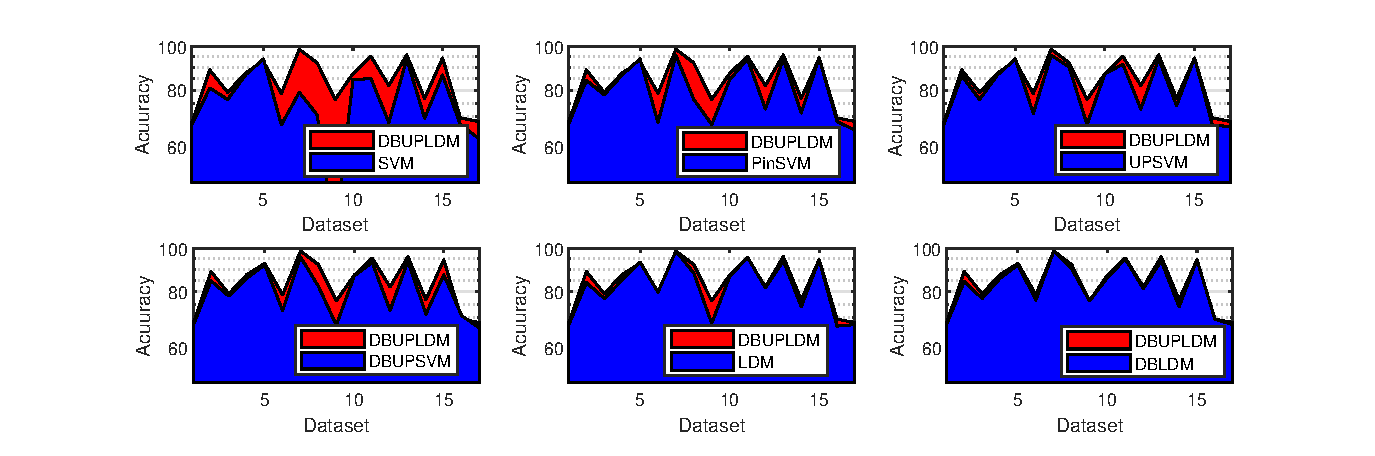
\includegraphics[width=15cm]{compare.eps}
    \caption{The performance comparison of SVM, LDM, PinSVM, UPSVM, and DBUPLDM in 17 dataset ($\rho = 0.125$).}
    \label{abb}
\end{figure*}

%%%move to Supplementary
% \begin{table*}
% \caption{Comparison of SVM, PinSVM, UPSVM, LDM, and DBUPLDM on noise-added UCI datasets}
% \renewcommand\arraystretch{1.3}
% \footnotesize
%   \centering
%    \setlength{\tabcolsep}{2mm}{
%     \resizebox{\textwidth}{!}{
%     \begin{tabular}{cccccccccccccccccccccccc}
%     \toprule
%     \multicolumn{2}{c}{\multirow{2}[4]{*}{Dataset}} & \multicolumn{4}{c}{SVM} & \multicolumn{4}{c}{LDM} & \multicolumn{4}{c}{PinSVM} & \multicolumn{4}{c}{UPSVM} & \multicolumn{4}{c}{\textbf{DBUPLDM}} \\
% \cmidrule{3-6}\cmidrule{7-10}\cmidrule{11-14}\cmidrule{15-18}\cmidrule{19-22}
%     \multicolumn{2}{c}{} & Accuracy & AUC & F1 & C & Accuracy & AUC & F1 & C & Accuracy & AUC & F1 & C & Accuracy & AUC & F1 & C & Accuracy & AUC & F1 & C \\
%     \midrule
%     \multirow{17}[4]{*}{$\varepsilon$ = 0.05}
%           & Monk1 & 57.87  & 59.87  & 57.37  & 0.25  & 61.11  & 63.11  & 60.61  & 4.00  & 60.65  & 62.65  & 60.15  & 0.03  & \textbf{63.43}  & 65.43  & 62.93  & 4.00  & 61.34  & 63.34  & 60.84  & 2.00  \\
%           & Monk2 & \textbf{67.13}  & 69.13  & 66.63  & 0.02  & \textbf{67.13}  & 69.13  & 66.63  & 0.02  & \textbf{67.13}  & 69.13  & 66.63  & 0.13  & \textbf{67.13}  & 69.13  & 66.63  & 0.02  & \textbf{67.13}  & 69.13  & 66.63  & 0.02  \\
%           & Monk3 & 72.45  & 74.45  & 71.95  & 0.50  & 72.45  & 74.45  & 71.95  & 0.50  & \textbf{73.38}  & 75.38  & 72.88  & 0.25  & \textbf{73.38}  & 75.38  & 72.88  & 0.25  & 71.99  & 73.99  & 71.49  & 4.00  \\
%           & Pima-Indian & 76.42  & 78.42  & 75.92  & 0.02  & 77.36  & 79.36  & 76.86  & 0.02  & 76.42  & 78.42  & 75.92  & 0.25  & 76.42  & 78.42  & 75.92  & 0.02  & \textbf{80.19}  & 82.19  & 79.69  & 8.00  \\
%           & WDBC  & 84.17  & 86.17  & 83.67  & 0.06  & \textbf{85.00}  & 87.00  & 84.50  & 0.03  & 84.17  & 86.17  & 83.67  & 0.06  & 84.17  & 86.17  & 83.67  & 0.06  & \textbf{85.00}  & 87.00  & 84.50  & 0.13  \\
%           & Echo  & 90.73  & 92.73  & 90.23  & 0.02  & 90.73  & 92.73  & 90.23  & 0.02  & 90.73  & 92.73  & 90.23  & 0.02  & 90.73  & 92.73  & 90.23  & 0.02  & \textbf{91.39}  & 93.39  & 90.89  & 8.00  \\
%           & Ionosphere & 67.09  & 69.09  & 66.59  & 0.02  & \textbf{78.85}  & 80.85  & 78.35  & 4.00  & 67.74  & 69.74  & 67.24  & 0.25  & 69.23  & 71.23  & 68.73  & 2.00  & 77.99  & 79.99  & 77.49  & 4.00  \\
%           & Heberman & 91.72  & 93.72  & 91.22  & 0.02  & \textbf{96.45}  & 98.45  & 95.95  & 8.00  & 92.90  & 94.90  & 92.40  & 0.13  & 95.86  & 97.86  & 95.36  & 0.25  & \textbf{96.45}  & 98.45  & 95.95  & 0.50  \\
%           & Statlog & 76.47  & 78.47  & 75.97  & 0.02  & 92.16  & 94.16  & 91.66  & 0.02  & 76.47  & 78.47  & 75.97  & 0.02  & 82.35  & 84.35  & 81.85  & 0.25  & \textbf{96.08}  & 98.08  & 95.58  & 1.00  \\
%           & Germans & 32.80  & 34.80  & 32.30  & 0.02  & 67.40  & 69.40  & 66.90  & 0.02  & 67.20  & 69.20  & 66.70  & 0.25  & 59.20  & 61.20  & 58.70  & 4.00  & \textbf{73.60}  & 75.60  & 73.10  & 4.00  \\
%           & Australian & 55.86  & 57.86 & 55.36  & 0.02  & 74.48  & 76.48  & 73.98  & 1.00  & 69.66  & 71.66  & 69.16  & 8.00  & \textbf{76.21}  & 78.21  & 75.71  & 8.00  & 75.52  & 77.52  & 75.02  & 0.25  \\
%           & Votes & 80.00  & 82.00  & 79.50  & 0.02  & 80.43  & 82.43  & 79.93  & 0.50  & 80.85  & 82.85  & 80.35  & 0.02  & \textbf{83.83}  & 85.83  & 83.33  & 0.02  & \textbf{83.83}  & 85.83  & 83.33  & 8.00  \\
%           & Diabetes & 67.91  & 69.91  & 67.41  & 0.02  & 80.22  & 82.22  & 79.72  & 2.00  & 72.39  & 74.39  & 71.89  & 0.03  & 72.76  & 74.76  & 72.26  & 4.00  & \textbf{80.60}  & 82.60  & 80.10  & 0.03  \\
%           & Fertility & \textbf{94.00}  & 96.00  & 93.50  & 0.02  & \textbf{94.00}  & 96.00  & 93.50  & 0.02  & \textbf{94.00}  & 96.00  & 93.50  & 0.02  & \textbf{94.00}  & 96.00  & 93.50  & 0.02  & \textbf{94.00}  & 96.00  & 93.50  & 0.02  \\
%           & Sonar & 58.33  & 60.33  & 57.83  & 0.25  & 62.04  & 64.04  & 61.54  & 8.00  & 59.26  & 61.26  & 58.76  & 0.25  & 62.04  & 64.04  & 61.54  & 0.50  & \textbf{64.81}  & 66.81  & 64.31  & 4.00  \\
%           & Ecoil & 51.18  & 53.18  & 50.68  & 0.02  & 54.33  & 56.33  & 53.83  & 0.03  & 59.84  & 61.84  & 59.34  & 0.06  & \textbf{62.20}  & 64.20  & 61.70  & 0.02  & 61.42  & 63.42  & 60.92  & 8.00  \\
%           & Plrx  & 67.07  & 69.07  & 66.57  & 0.02  & 67.07  & 69.07  & 66.57  & 0.02  & 67.07  & 69.07  & 66.57  & 0.02  & 68.29  & 70.29  & 67.79  & 0.06  & \textbf{70.73}  & 72.73  & 70.23  & 8.00  \\
% \cmidrule{2-22}
%           & \textbf{Ave. } & 70.07  & 72.07  & 69.57  &   & 76.54  & 78.54  & 76.04  &   & 74.11  & 76.11  & 73.61  &   & 75.37  & 77.37  & 74.87  &   & \textbf{78.36 } & 80.36  & 77.86  &   \\
%     \midrule
%     \multirow{17}[4]{*}{$\varepsilon$ = 0.1}
%           & Monk1 & 57.64  & 59.64  & 57.14  & 0.25  & 61.11  & 63.11  & 60.61  & 4.00  & 60.42  & 62.42  & 59.92  & 0.02  & \textbf{63.43}  & 65.43  & 62.93  & 4.00  & 61.34  & 63.34  & 60.84  & 2.00  \\
%           & Monk2 & \textbf{67.13}  & 69.13  & 66.63  & 0.02  & \textbf{67.13}  & 69.13  & 66.63  & 0.02  & \textbf{67.13}  & 69.13  & 66.63  & 0.13  & \textbf{67.13}  & 69.13  & 66.63  & 0.02  & \textbf{67.13}  & 69.13  & 66.63  & 0.02  \\
%           & Monk3 & 71.76  & 73.76  & 71.26  & 0.25  & 72.22  & 74.22  & 71.72  & 0.50  & \textbf{73.38}  & 75.38  & 72.88  & 0.50  & \textbf{73.38}  & 75.38  & 72.88  & 0.50  & 71.99  & 73.99  & 71.49  & 4.00  \\
%           & Pima-Indian & 76.42  & 78.42  & 75.92  & 0.02  & 77.36  & 79.36  & 76.86  & 0.02  & 76.42  & 78.42  & 75.92  & 0.25  & 76.42  & 78.42  & 75.92  & 0.02  & \textbf{80.19}  & 82.19  & 79.69  & 8.00  \\
%           & WDBC  & 84.17  & 86.17  & 83.67  & 0.06  & \textbf{85.00}  & 87.00  & 84.50  & 0.03  & 84.17  & 86.17  & 83.67  & 0.06  & 84.17  & 86.17  & 83.67  & 0.06  & \textbf{85.00}  & 87.00  & 84.50  & 0.13  \\
%           & Echo  & 90.73  & 92.73  & 90.23  & 0.02  & 90.73  & 92.73  & 90.23  & 0.02  & 90.73  & 92.73  & 90.23  & 0.02  & \textbf{91.39}  & 93.39  & 90.89  & 0.03  & \textbf{91.39}  & 93.39  & 90.89  & 8.00  \\
%           & Ionosphere & 67.09  & 69.09  & 66.59  & 0.02  & \textbf{78.85}  & 80.85  & 78.35  & 8.00  & 69.87  & 71.87  & 69.37  & 4.00  & 69.02  & 71.02  & 68.52  & 2.00  & 77.78  & 79.78  & 77.28  & 4.00  \\
%           & Heberman & 91.72  & 93.72  & 91.22  & 0.02  & \textbf{96.45}  & 98.45  & 95.95  & 8.00  & 95.27  & 97.27  & 94.77  & 0.03  & 95.86  & 97.86  & 95.36  & 0.25  & \textbf{96.45}  & 98.45  & 95.95  & 0.50  \\
%           & Statlog & 76.47  & 78.47  & 75.97  & 0.02  & 94.12  & 96.12  & 93.62  & 0.25  & 76.47  & 78.47  & 75.97  & 0.02  & 82.35  & 84.35  & 81.85  & 0.25  & \textbf{96.08}  & 98.08  & 95.58  & 1.00  \\
%           & Germans & 32.80  & 34.80  & 32.30  & 0.02  & 67.40  & 69.40  & 66.90  & 0.02  & 67.20  & 69.20  & 66.70  & 0.25  & 59.20  & 61.20  & 58.70  & 2.00  & \textbf{73.60}  & 75.60  & 73.10  & 4.00  \\
%           & Australian & 55.86  & 57.86  & 55.36  & 0.02  & 74.48  & 76.48  & 73.98  & 1.00  & 65.86  & 67.86  & 65.36  & 0.03  & \textbf{75.86}  & 77.86  & 75.36  & 8.00  & 75.52  & 77.52  & 75.02  & 0.25  \\
%           & Votes & 82.13  & 84.13  & 81.63  & 0.02  & 80.85  & 82.85  & 80.35  & 0.25  & 82.13  & 84.13  & 81.63  & 0.02  & \textbf{84.26}  & 86.26  & 83.76  & 0.02  & 83.83  & 85.83  & 83.33  & 8.00  \\
%           & Diabetes & 67.91  & 69.91  & 67.41  & 0.03  & 80.22  & 82.22  & 79.72  & 2.00  & 69.03  & 71.03  & 68.53  & 0.06  & 72.76  & 74.76  & 72.26  & 4.00  & \textbf{80.60}  & 82.60  & 80.10  & 0.03  \\
%           & Fertility & \textbf{94.00}  & 96.00  & 93.50  & 0.02  & \textbf{94.00}  & 96.00  & 93.50  & 0.02  & \textbf{94.00}  & 96.00  & 93.50  & 0.02  & \textbf{94.00}  & 96.00  & 93.50  & 0.02  & \textbf{94.00}  & 96.00  & 93.50  & 0.02  \\
%           & Sonar & 59.26  & 61.26  & 58.76  & 0.25  & 62.04  & 64.04  & 61.54  & 8.00  & 59.26  & 61.26  & 58.76  & 0.02  & 62.04  & 64.04  & 61.54  & 0.25  & \textbf{64.81}  & 66.81  & 64.31  & 2.00  \\
%           & Ecoil & 51.18  & 53.18  & 50.68  & 0.02  & 54.33  & 56.33  & 53.83  & 0.03  & \textbf{62.20}  & 64.20  & 61.70  & 8.00  & \textbf{62.20}  & 64.20  & 61.70  & 0.02  & 61.42  & 63.42  & 60.92  & 8.00  \\
%           & Plrx  & 67.07  & 69.07  & 66.57  & 0.02  & 67.07  & 69.07  & 66.57  & 0.02  & 67.07  & 69.07  & 66.57  & 0.02  & 68.29  & 70.29  & 67.79  & 0.06  & \textbf{70.73}  & 72.73  & 70.23  & 8.00  \\
% \cmidrule{2-22}
%           & \textbf{Ave. } & 70.20  & 72.20  & 69.70  &   & 76.67  & 78.67  & 76.17  &   & 74.15  & 76.15  & 73.65  &   & 75.40  & 77.40  & 74.90  &   & \textbf{78.34}  & 80.34  & 77.84  &   \\
%     \bottomrule
%     \end{tabular}}}%
%     \label{ucin}
% \end{table*}%

%%%TODO



\subsection{Experiments on UCI datasets}
\label{UCI_nor}

In this subsection, we compare DBUPLDM with four other benchmark algorithms. We select 17 UCI datasets with varying features and imbalance ratios and add Gaussian white noise to these datasets to investigate the anti-noise performance of DBUPLDM. For ``Monk1", ``Monk2", ``Monk3", and ``Spect" data, UCI provides training and test sets. For other datasets, we divide each of them into the training set and test set in a certain proportion.

As shown in Table \ref{dataset}, there is data imbalance in almost all training sets. To fully validate the performance of our model on imbalanced datasets, we adjust this dataset imbalance by setting different parameters $\eta$: setting $\eta$ to 1, 1/2, 1/4, 1/8, 1/16, 1/32, and 1/64, which means the ratio of the minority class to the majority class. The SVM, PinSVM, UPSVM, and LDM algorithms are tested ten times each for all datasets, and the average accuracy is selected as the final comparison criterion. The experimental results are presented in Tables \ref{uci1} and Supplementary TABLE S1.



{\color{orange}Tables \ref{uci1} and Supplementary TABLE S1. demonstrate that DBUPLDM achieves the best overall performance in terms of Accuracy, AUC, and F1-score across all 17 datasets. Regardless of the adjustment of parameter \(\eta\), DBUPLDM consistently maintains the highest average levels in these three metrics. Specifically, as \(\eta\) decreases, the Accuracy, AUC, and F1-score of DBUPLDM tend to first increase and then decrease, with the optimal performance observed at \(\eta = 0.125\). Compared with SVM and some of its improved versions (i.e., PinSVM and UPSVM), LDM has a higher accuracy because it takes into account the marginal distribution theory and adds a second-order statistic to the model. However, due to its use of the hinge loss function, LDM is not suitable for imbalanced classification tasks, resulting in its Accuracy, AUC, and F1-score being lower than those of DBUPLDM. Interestingly, algorithms with pinball loss functions (PinSVM, UPSVM, and DBUPLDM) perform better in terms of Accuracy, AUC, and F1-score when \(\tau\) takes negative values.}

To provide a more visual representation of the excellent performance of DBUPLDM, we have summarized the information from Table \ref{uci1}  and Supplementary TABLE S1 in Table \ref{win}.



Table \ref{win} presents the number of accuracy wins, draws, and losses of each algorithm concerning the 17 datasets. The results are denoted as ``WIN", ``DRAW", and ``LOSS" to indicate each algorithm's performance when compared to others. DBUPLDM achieves the best performance in this analysis. Since 17 datasets were selected and each algorithm needs to be compared with the remaining 4 algorithms, the sum of ``WIN", ``DRAW", and ``LOSS" for each algorithm is 17$\times$4=68. Therefore, the total sum across the six parameters $\eta$ is 68$\times$6=408. The average win rate of DBUPLDM is 79\% (324/408) with a loss rate of only 8\% (35/408). Specifically for each of the $\eta$-parameters, the performance of DBUPLDM maintains a win rate of higher than 75\% (51/68) and a loss rate of always less than 10\%. These results demonstrate the consistently outstanding performance of our proposed DBUPLDM.

{\color{red}To validate the statistical significance of the observed performance differences, we conducted two-sided Wilcoxon signed-rank tests comparing the win counts of DBUPLDM against four baseline models (SVM, UPSVM, PinSVM, and LDM). Each comparison pairs the two models' win counts across the six $\eta$ settings ($n=6$ paired observations; see the WIN rows of Table~\ref{win}). DBUPLDM records more wins than each baseline at every $\eta$ value, so all six paired differences favor DBUPLDM and the exact two-sided p-value is $0.03125$ in all four comparisons. The matched-pairs rank-biserial correlation is $1.00$ and the standardized effect size is $r=Z/\sqrt{n}\approx 0.90$ ($Z\approx 2.20$), both indicating a large effect that reinforces the robustness of DBUPLDM's superiority beyond random fluctuations.}




% \begin{figure*}[htbp]
%   	\centering 
% 	\subfigure[imbalance ratio = 2]{
% 	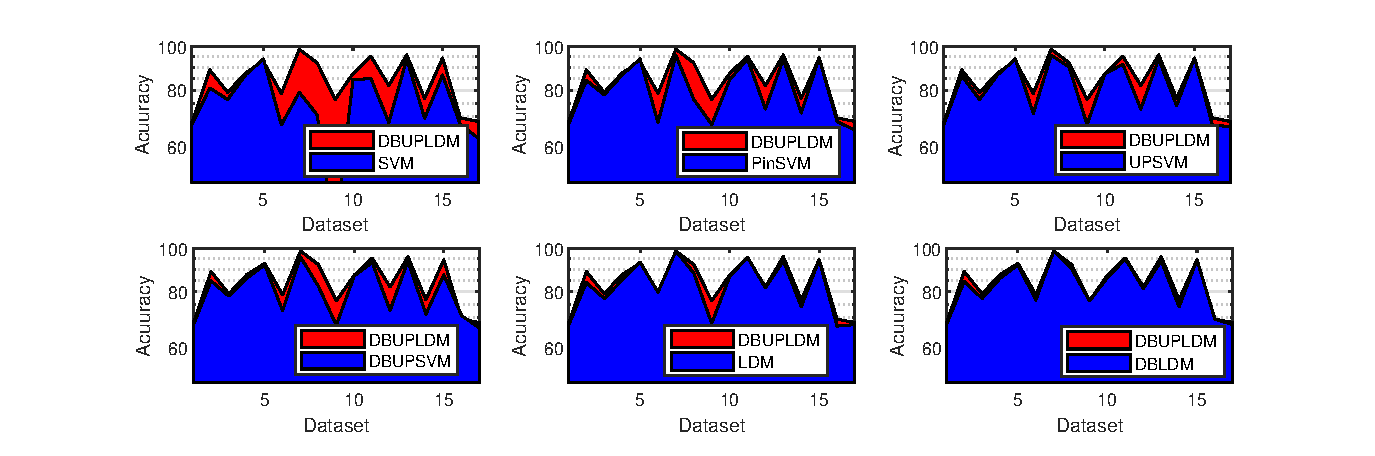
\includegraphics[width=7cm]{compare.eps}
% }
% 	\subfigure[imbalance ratio = 3]{
% 	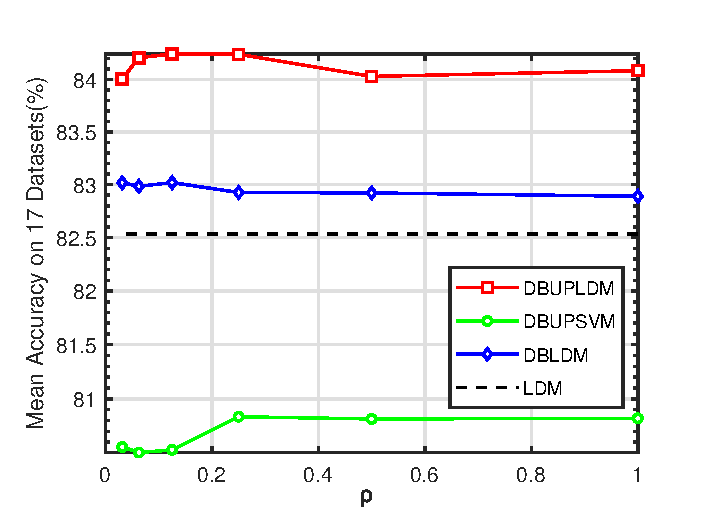
\includegraphics[width=7cm]{compare_p.eps}
% }
% 	\caption{The performance comparison of SVM, LDM, PinSVM, UPSVM, and DBUPLDM in 17 data sets.}
% \end{figure*}

\begin{table*}[htbp]
\renewcommand\arraystretch{1}
  \centering
      \caption{Performance metrics for various algorithms on imbalanced datasets}\label{metrics}
    \setlength{\tabcolsep}{3 mm}
    \small
    \begin{tabular}{cccccccc}
    \toprule
    \multicolumn{1}{c}{Dataset} & Metrics & SVM   & LDM   & PSVM  & UPSVM & CSLDM & DBUPLDM \\
    \midrule
    \multicolumn{1}{c}{\multirow{3}[2]{*}{Bank}} & AUC   & 52.79  & \textbf{53.37 } & 52.79  & 52.79 & 48.13 & 52.79 \\
          & F-measure & 0.00  & 5.45  & 0.00  & 28.74 & 18.37 & \textbf{33.06} \\
          & G-means & 0.00  & 17.07  & 0.00  & 0.00  & \textbf{38.75} & 0.00 \\
    \midrule
    \multicolumn{1}{c}{\multirow{3}[2]{*}{Thyroid\_Diff}} & AUC   & 49.91  & 48.03  & 48.03  & 48.03  & \textbf{57.23 } & 49.22  \\
          & F-measure & 44.16  & 0.00  & 47.67  & 46.51  & 40.34  & \textbf{48.70 } \\
          & G-means & 27.54  & 0.00  & 0.00  & 0.00  & \textbf{55.81 } & 50.38  \\
    \midrule
    \multicolumn{1}{c}{\multirow{3}[2]{*}{Phoneme}} & AUC   & \textbf{51.38 } & 51.33  & 51.33 & 51.33 & 43.13 & 51.33 \\
          & F-measure & 22.04  & 0.00  & 22.04 & \textbf{22.51} & 14.04 & 22.00 \\
          & G-means & 5.11  & 0.00  & 0.00  & 0.00  & \textbf{40.16} & 0.00 \\
    \midrule
    \multicolumn{1}{c}{\multirow{3}[2]{*}{Website\_Phishing}} & AUC   & 51.84  & 51.19  & 51.84 & 51.84 & \textbf{52.90} & 51.19 \\
          & F-measure & 3.77  & 0.00  & 14.72 & 18.37 & 12.80 & \textbf{19.05} \\
          & G-means & 13.99  & 0.00  & 13.99 & 13.99 & \textbf{37.46} & 0.00 \\
    \midrule
    \multicolumn{1}{c}{\multirow{3}[2]{*}{Oil\_Spill}} & AUC   & \textbf{42.49 } & \textbf{42.49 } & \textbf{42.49} & \textbf{42.49} & 42.06 & \textbf{42.49} \\
          & F-measure & 0.00  & 0.00  & 0.00  & \textbf{15.00} & 0.00  & 10.94 \\
          & G-means & 0.00  & 0.00  & 0.00  & 0.00  & 0.00  & 0.00 \\
    \midrule
    \multicolumn{1}{c}{\multirow{3}[2]{*}{Pharyngitis}} & AUC   & 53.92  & 53.92 & 53.92 & 53.92 & 49.94 & \textbf{56.03} \\
          & F-measure & 94.36  & 94.36 & 94.36 & 94.36 & 56.56 & \textbf{94.51} \\
          & G-means & 0.00  & 0.00  & 0.00  & 0.00  & \textbf{48.03} & 32.44 \\
    \midrule
    \multicolumn{1}{c}{\multirow{3}[2]{*}{Blood\_Transfusion\_Service}} & AUC   & \textbf{49.01 } & \textbf{49.01} & \textbf{49.01} & \textbf{49.01} & 45.31 & \textbf{49.01} \\
          & F-measure & 38.44  & 0.00  & 38.44 & 38.70 & 26.98 & \textbf{39.34} \\
          & G-means & 0.00  & 0.00  & 0.00  & 0.00  & \textbf{46.36} & 0.00 \\
    \midrule
    \multirow{3}[2]{*}{\textbf{Ave. }} & AUC   & 50.19  & 49.91  & 49.92  & 49.92  & 48.39  & \textbf{50.29 } \\
          & F-measure & 28.97  & 14.26  & 31.03  & 37.74  & 24.16  & \textbf{38.23 } \\
          & G-means & 6.66  & 2.44  & 2.00  & 2.00  & \textbf{38.08 } & 11.83  \\
    \bottomrule
    \end{tabular}%
\end{table*}%

In order to verify whether the superior performance of DBUPLDM stems from our proposed dual balanced method and unified pinball loss function, an ablation experiment is conducted on the basis of the above experiments. The parameter $\rho$ is set to 0.125, and the experimental results are presented in Table \ref{ab} and illustrated in Fig. \ref{abb}.

\begin{figure}
   	\centering 
	\subfigure[Monk1 dataset]{
	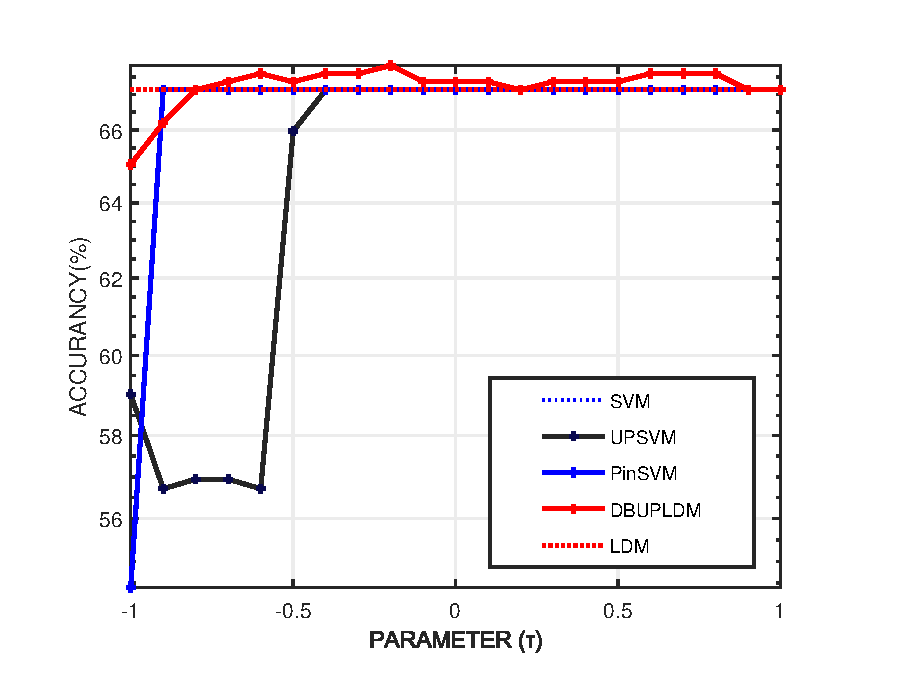
\includegraphics[width=5cm]{2.eps}
}\hspace{-5mm}
   	\subfigure[Monk 2 dataset]{
	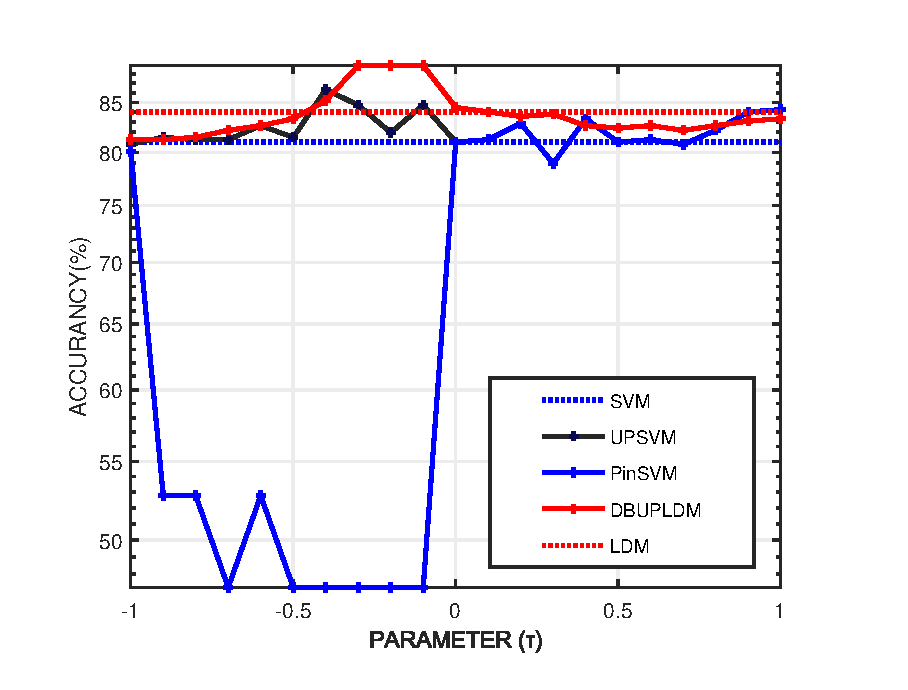
\includegraphics[width=5cm]{3.eps}
}\hspace{-5mm}
	\subfigure[Monk 3 dataset]{
	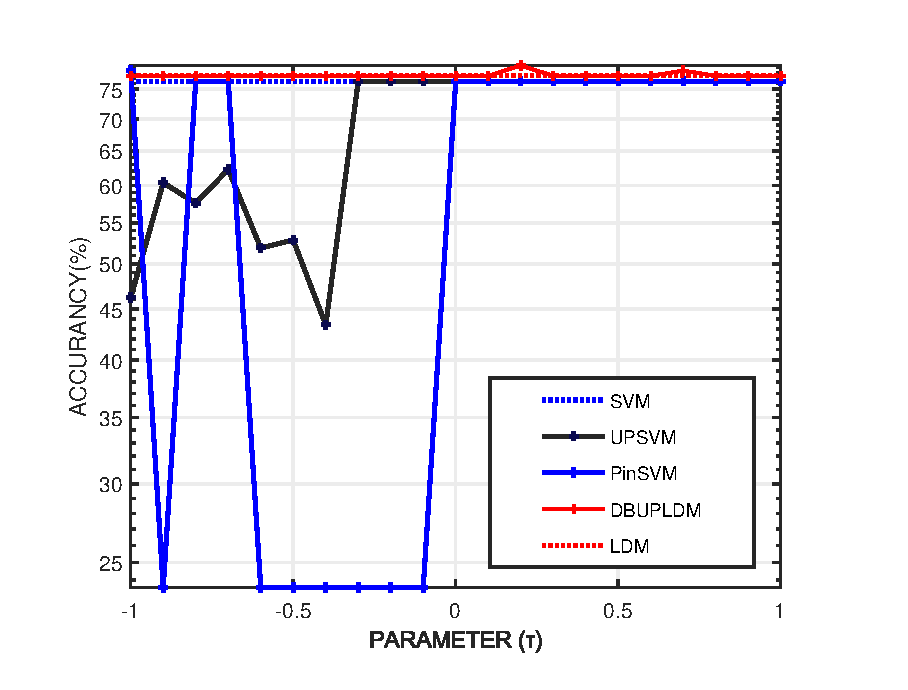
\includegraphics[width=5cm]{5.eps}
}\hspace{-5mm}
	\subfigure[Echo dataset]{
	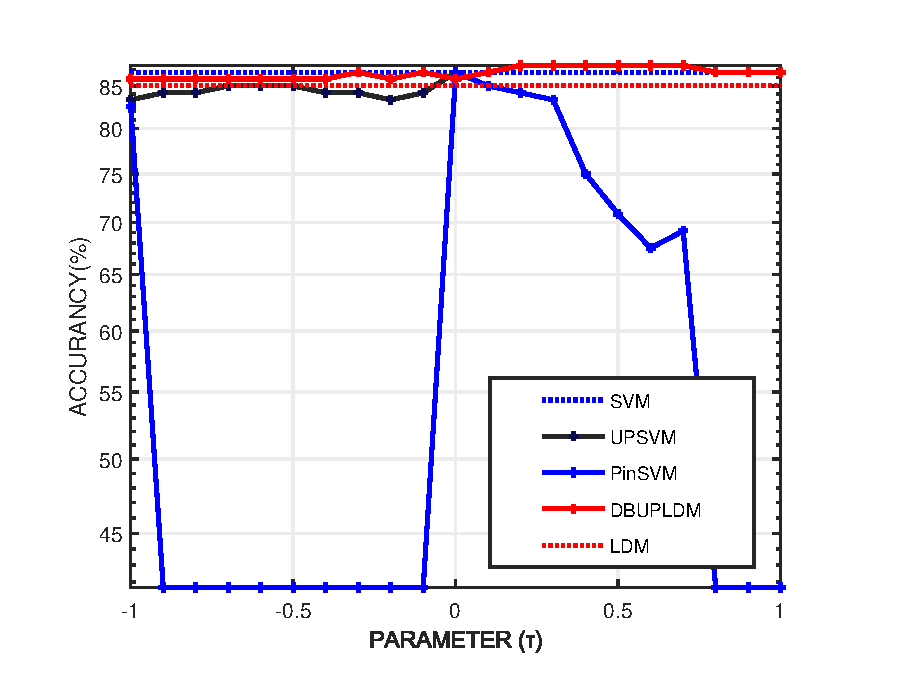
\includegraphics[width=5cm]{6.eps}
}\hspace{-5mm}
	\subfigure[Germans dataset]{
	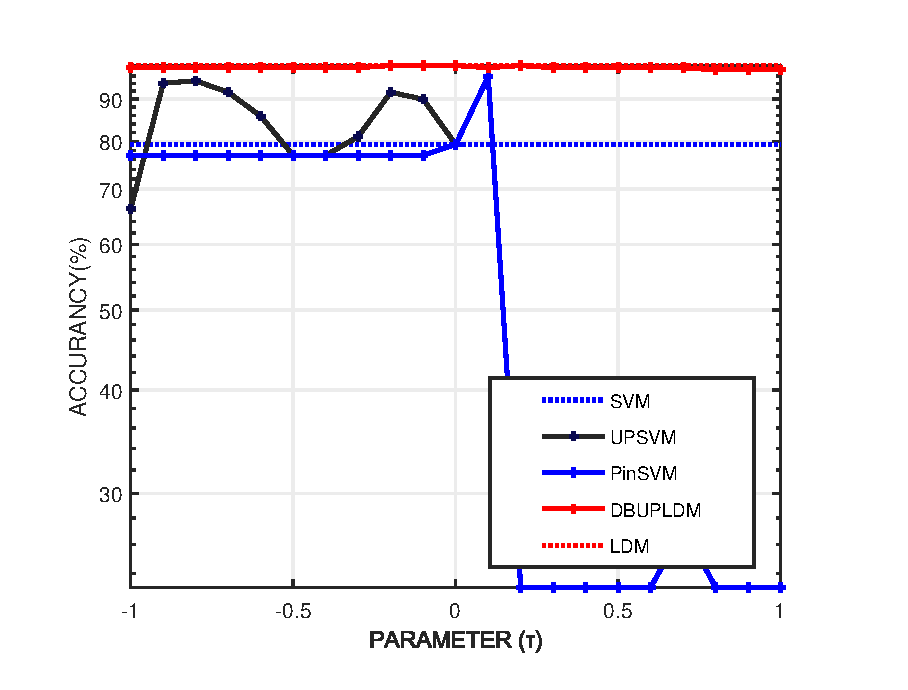
\includegraphics[width=5cm]{9.eps}
}\hspace{-5mm}
	\subfigure[BUPA dataset]{
	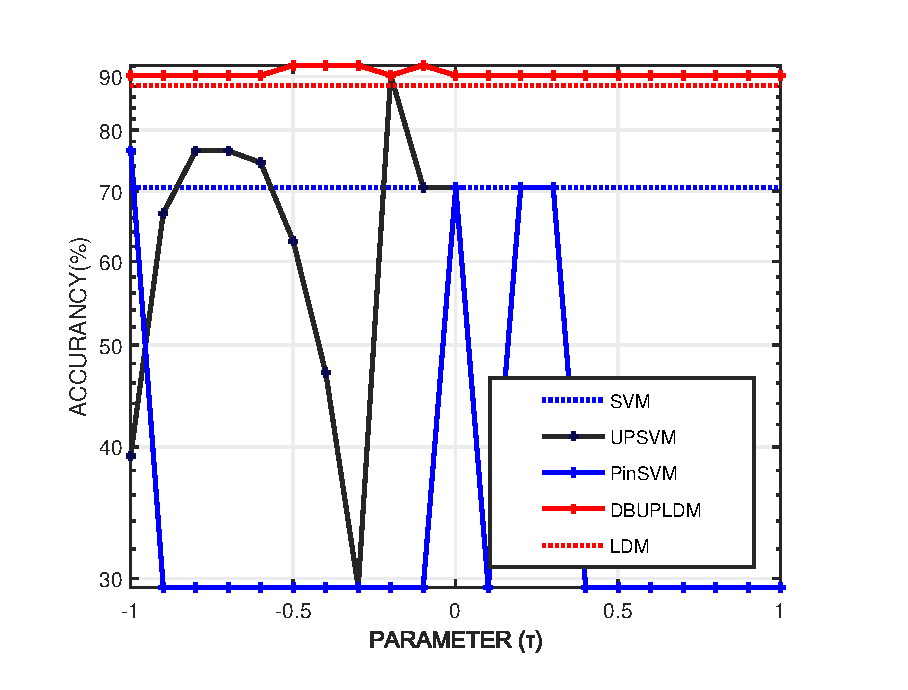
\includegraphics[width=5cm]{10.eps}
}\hspace{-5mm}
	\subfigure[Daibetes dataset]{
	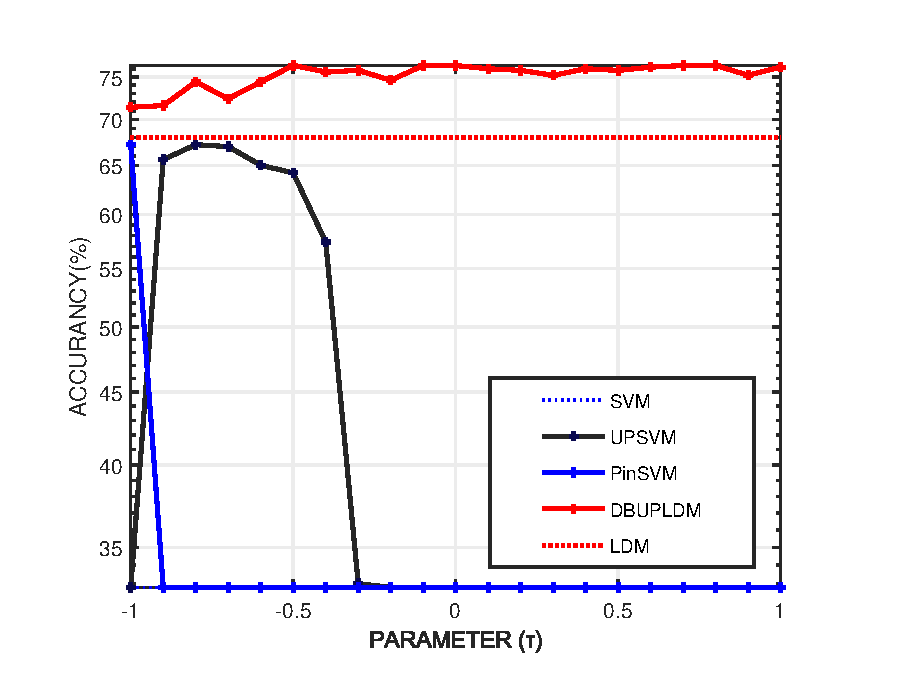
\includegraphics[width=5cm]{11.eps}
}\hspace{-5mm}
	\subfigure[Sonar dataset]{
	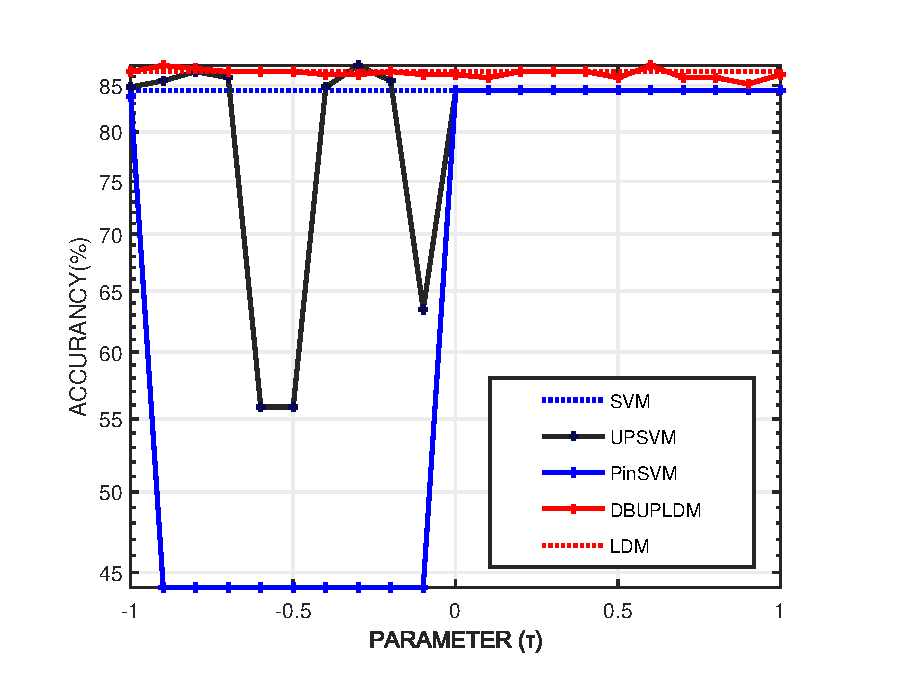
\includegraphics[width=5cm]{12.eps}
}\hspace{-5mm}
	\subfigure[Prlx dataset]{
	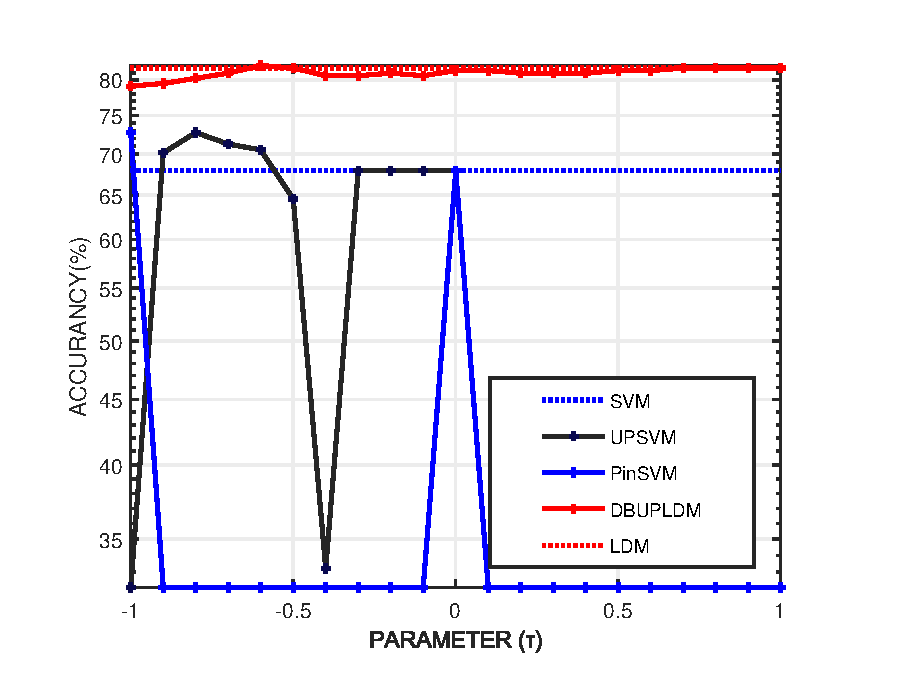
\includegraphics[width=5cm]{15.eps}
}\hspace{-5mm}
	\subfigure[Prlx dataset]{
	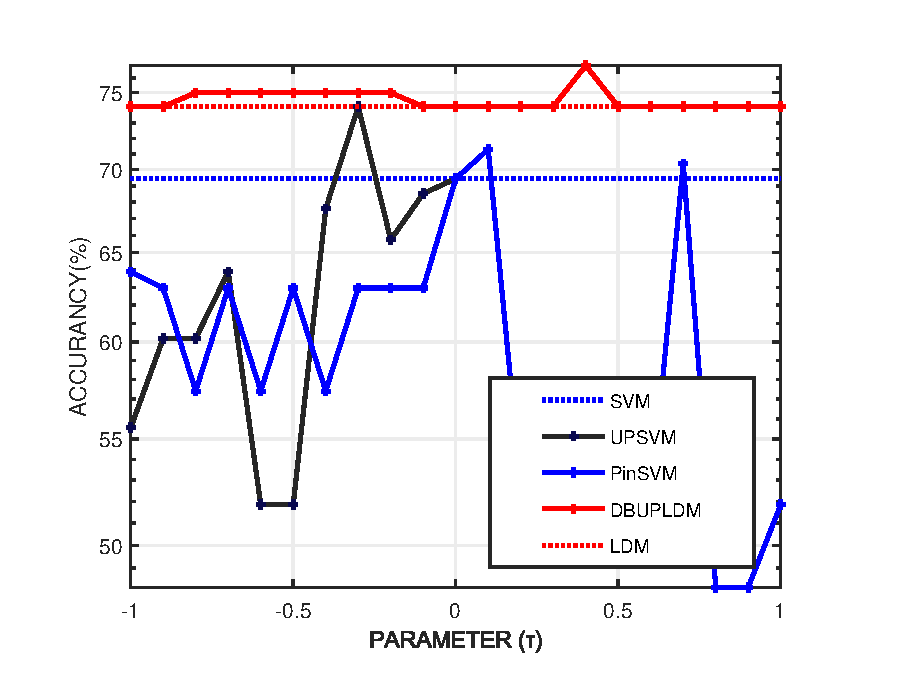
\includegraphics[width=5cm]{17.eps}
}\hspace{-5mm}
	\subfigure[Prlx dataset]{
	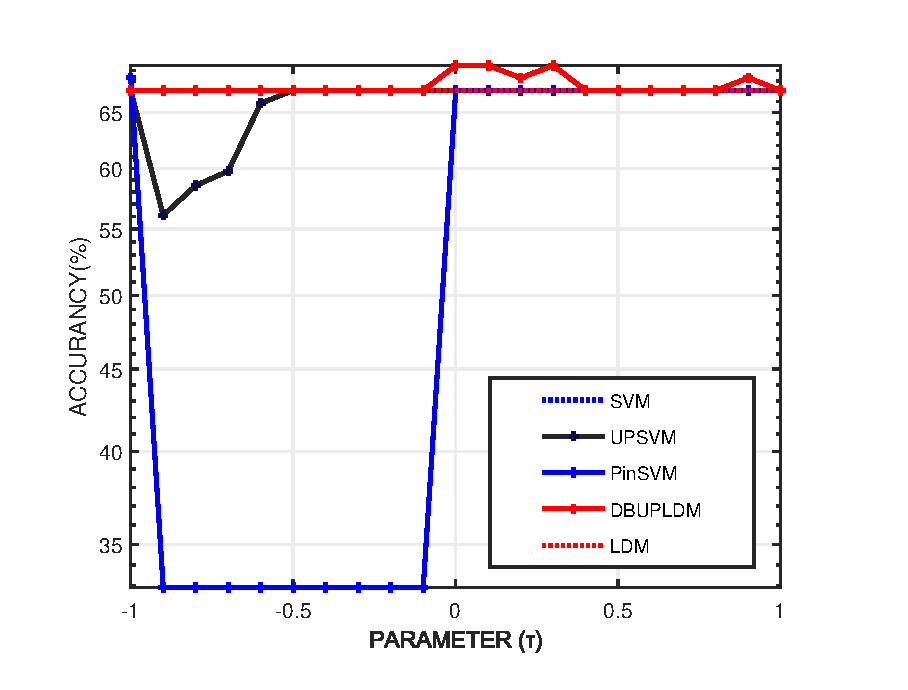
\includegraphics[width=5cm]{19.eps}
}\hspace{-5mm}
	\subfigure[Prlx dataset]{
	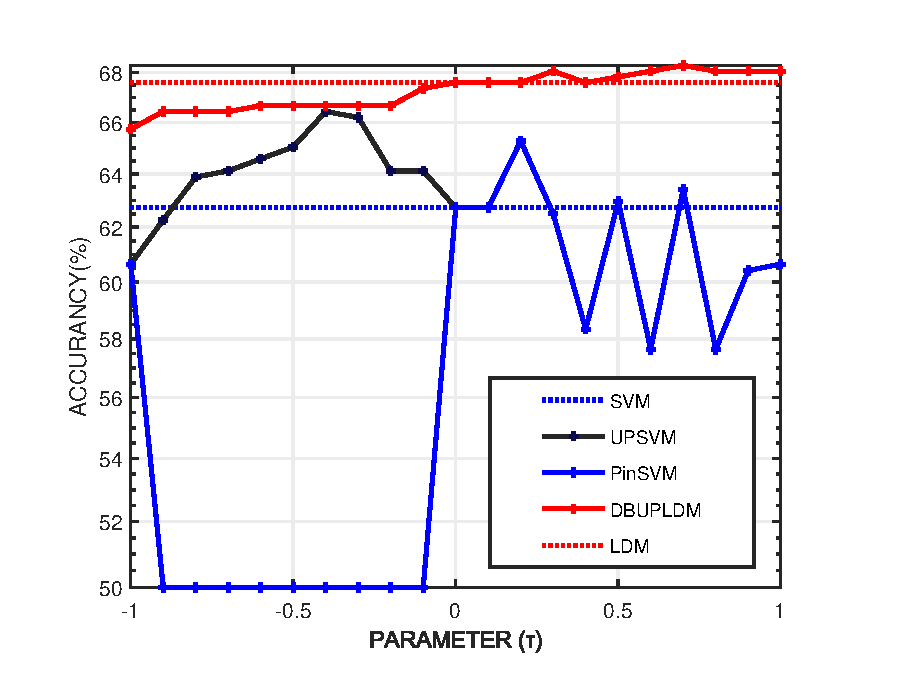
\includegraphics[width=5cm]{20.eps}
}
	\caption{The parameter sensitivity performance of SVM, LDM, Pin-SVM, UPSVM, and DBUPLDM in different datasets.)}
	\label{acc}
\end{figure}

The comparison metric for the ablation experiments is formulated as the average performance of the algorithms on the 17 datasets, measured by their average accuracy. As can be seen from Table \ref{ab} of the ablation experiment results, the base model without any treatment (LDM) has the worst performance, while adding the balanced factors (DBLDM) or modifying the loss function (UPLDM) leads to an improvement in classification accuracy by 0.48\% and 1\%, respectively. Moreover, when both the balanced factors and modified loss function are added, accuracy is improved by 1.7\%.

Fig. \ref{abb} illustrates the accuracy improvement of DBUPLDM compared to other algorithms on the 17 datasets. SVM has the most significant improvement, followed by PinSVM, UPSVM, DBUPSVM, LDM, and DBLDM. These results demonstrate that the proposed balanced factors and unified pinball loss function play a crucial role in improving the performance of the proposed algorithm. Furthermore, the overall accuracy of LDM and DBUPLDM outperforms that of SVM and UPSVM, respectively. This observation highlights the effectiveness of considering the overall distribution of samples to improve algorithm accuracy.

In conclusion, LDM outperforms SVM, and the UP loss leads to better generalization performance than hinge loss. The proposed DBUPLDM has better classification performance than the other algorithms, due to the incorporation of dual balanced factors and the unified pinball loss function.

% Based on the experimental results, we compare the CPU time consumption of DBUPLDM and LDM in classifying the above datasets. The experimental results are shown in Table \ref{tabel2}.

% \begin{table}[htbp]
% \scriptsize
% \renewcommand\arraystretch{1.3}
%   \centering
%   \caption{CPU time consumption of LDM and DBUPLDM}
%   \setlength{\tabcolsep}{7mm}{
%     \begin{tabular}{cccccc}
%     \toprule
%     Dataset & LDM   & DBUPLDM & Dataset & LDM   & DBUPLDM \\
%     \midrule
%     Monk 2 & \textbf{2.25 } & 2.35 & Bupa  & 4.99  & \textbf{4.75} \\
%     Monk 3 & 2.35  & \textbf{2.08} & Votes & 3.32  & \textbf{2.09} \\
%     Heberman & 2.32  & \textbf{1.98} & Diabetes & 20.56  & \textbf{14.95} \\
%     Statlog & 2.65  & \textbf{2.64} & Fertility & 0.60  & \textbf{0.55} \\
%     Pima-Indian & 6.60  & \textbf{5.72} & Plrx  & 1.28  & \textbf{1.18} \\
%     Echo  & \textbf{0.96 } & \textbf{0.96 } & Monk 1 & 2.00  & \textbf{1.93} \\
%     WDBC  & \textbf{12.90 } & 13.18 & Original & \textbf{6.53 } & 7.10 \\
%     Australian & \textbf{15.34 } & 18.93 & BUPA  & 4.20  & \textbf{3.67} \\
%     \bottomrule
%     \end{tabular}}%
%   \label{tabel2}%
% \end{table}%

% It can be seen from Table \ref{tabel2} that on 16 datasets, the time consumption of DBUPLDM on 13 datasets is not much different from that of traditional LDM. From the previous analysis, DBUPLDM has the same number of unknown parameters and constraints as LDM. Since $\tau$ is a hyperparameter, it does not impose a time burden on the training process. Therefore, DBUPLDM also has excellent time efficiency.

{\color{blue}To further validate the effectiveness and robustness of our proposed model DBUPLDM, we conducted a comprehensive comparison against a deep learning-based imbalanced learning technique: MLP with Focal Loss\citep{lin2017focal}. Specifically, we selected the variant of DBUPLDM that achieved the highest average accuracy and compared it with MLP with Focal Loss under consistent settings. This evaluation aims to highlight the superior performance of DBUPLDM across various datasets with different imbalance characteristics.}

{\color{magenta}To ensure reproducibility and fair comparison, we provide detailed specifications for all baseline models, including complete network architectures, optimization frameworks, hyperparameter tuning procedures, and regularization strategies. The MLP+Focal Loss baseline was implemented as a fully connected neural network with two hidden layers (128 and 64 neurons) and \texttt{ReLU} activation functions. The released implementation applies batch normalization and dropout 0.3 after each hidden layer. The model was trained using Adam with learning rate 0.001, batch size 32, and $L_2$ weight decay $1\times10^{-5}$. Focal Loss uses class-frequency weights, focusing parameter $\gamma=2.0$, and mean reduction. Training uses a maximum of 100 epochs with early stopping (patience 15) and ReduceLROnPlateau learning-rate decay by factor 0.5 after 5 epochs without improvement. The released implementation records the fixed random seed, configuration, and fold-level predictions for every run.}

{\color{red}We additionally evaluate three recent imbalance-learning baselines using tabular architectures. DeepSMOTE uses an encoder--decoder with latent dimension 128 and encoder widths 256--128--64; minority samples are interpolated among latent-space nearest neighbors and decoded before classification, with reconstruction penalty weight 0.1. LDAM uses the same two-hidden-layer tabular MLP backbone as the other neural baselines, class-dependent margins with maximum margin $\Delta=0.5$, scale 30, and deferred class reweighting after epoch 160. Balanced Softmax uses the same MLP backbone and adds the logarithm of the training class counts to the logits with temperature $T=1.0$. All three baselines use Adam (learning rate 0.001, weight decay $1\times10^{-5}$), batch size 32, at most 200 epochs, early stopping patience 10, and stratified 5-fold cross-validation. Early stopping, learning-rate scheduling, and checkpoint selection use a held-out selection split inside each training fold, so each reported fold is evaluated only once at the end. The released code reports the seed and each fold's Accuracy, AUC, and F1-score; the source code and datasets are available at \url{https://github.com/Jlchen08/dbupldm_code}.}

\begin{table*}[htbp]
  \centering
  \footnotesize
  \caption{{\color{red}Performance Comparison (Acc/AUC/F1-score) Among DBUPLDM, MLP+Focal Loss, DeepSMOTE, Tabular-MLP LDAM, and Tabular-MLP Balanced Softmax on 17 Benchmark Datasets}}
  \vspace{2mm}
  \setlength{\tabcolsep}{1mm}{ % 缩小列间距适配多指标
    \begin{tabular}{lcccccc}
    \toprule
    \textbf{Model} & Monk1 & Monk2 & Monk3 & Pima & WDBC & Echo \\
    \midrule
    \textbf{DBUPLDM} & 68.29/72.13/0.69 & 67.82/78.64/0.76 & 88.89/92.43/0.89 & \textbf{79.25}/79.34/0.72 & 87.50/91.43/0.89 & \textbf{92.72}/83.66/0.76 \\
    MLP+Focal        & {\color{red}92.80}/{\color{red}98.59}/{\color{red}0.93} & {\color{red}77.38}/{\color{red}93.28}/{\color{red}0.78} & {\color{red}96.03}/{\color{red}99.26}/{\color{red}0.96} & {\color{red}70.95}/{\color{red}82.56}/{\color{red}0.71} & {\color{red}96.14}/{\color{red}99.62}/{\color{red}0.96} & {\color{red}77.81}/{\color{red}88.28}/{\color{red}0.78} \\
    DeepSMOTE        & {\color{red}93.71}/{\color{red}98.85}/{\color{red}0.94} & \textbf{\color{red}87.38}/{\color{red}94.36}/\textbf{\color{red}0.88} & \textbf{\color{red}96.93}/\textbf{\color{red}99.52}/\textbf{\color{red}0.97} & {\color{red}74.86}/{\color{red}82.79}/{\color{red}0.75} & {\color{red}96.31}/{\color{red}99.36}/{\color{red}0.96} & {\color{red}77.01}/{\color{red}85.42}/{\color{red}0.78} \\
    LDAM             & {\color{red}92.99}/{\color{red}98.62}/{\color{red}0.93} & {\color{red}83.20}/{\color{red}90.57}/{\color{red}0.83} & {\color{red}96.03}/{\color{red}99.21}/{\color{red}0.96} & {\color{red}77.47}/\textbf{\color{red}83.11}/\textbf{\color{red}0.77} & \textbf{\color{red}97.36}/{\color{red}99.60}/\textbf{\color{red}0.97} & {\color{red}84.64}/\textbf{\color{red}88.75}/\textbf{\color{red}0.85} \\
    Balanced Softmax & \textbf{\color{red}96.94}/\textbf{\color{red}99.72}/\textbf{\color{red}0.97} & {\color{red}86.69}/\textbf{\color{red}96.08}/{\color{red}0.87} & {\color{red}96.57}/{\color{red}99.46}/{\color{red}0.97} & {\color{red}73.69}/{\color{red}83.01}/{\color{red}0.74} & {\color{red}96.67}/\textbf{\color{red}99.63}/{\color{red}0.97} & {\color{red}82.39}/{\color{red}87.99}/{\color{red}0.83} \\
    \midrule
    \textbf{Model} & Iono & Habe & Stat & Germ & Aust & Vote \\
    \midrule
    \textbf{DBUPLDM} & 78.85/89.23/0.76 & \textbf{98.82}/\textbf{85.51}/\textbf{0.86} & \textbf{92.16}/79.46/\textbf{0.91} & \textbf{76.40}/73.21/\textbf{0.78} & \textbf{87.24}/83.44/0.84 & \textbf{95.32}/\textbf{87.29}/\textbf{0.79} \\
    MLP+Focal        & {\color{red}94.29}/{\color{red}98.79}/{\color{red}0.94} & {\color{red}36.30}/{\color{red}67.95}/{\color{red}0.31} & {\color{red}81.11}/{\color{red}87.61}/{\color{red}0.81} & {\color{red}60.90}/{\color{red}77.54}/{\color{red}0.62} & {\color{red}85.51}/{\color{red}92.44}/\textbf{\color{red}0.86} & {\color{red}58.62}/{\color{red}64.71}/{\color{red}0.58} \\
    DeepSMOTE        & \textbf{\color{red}94.86}/{\color{red}98.58}/\textbf{\color{red}0.95} & {\color{red}71.57}/{\color{red}69.76}/{\color{red}0.71} & {\color{red}81.48}/{\color{red}89.33}/{\color{red}0.81} & {\color{red}70.90}/{\color{red}77.13}/{\color{red}0.72} & {\color{red}85.94}/{\color{red}92.75}/{\color{red}0.86} & {\color{red}60.92}/{\color{red}64.52}/{\color{red}0.61} \\
    LDAM             & {\color{red}93.73}/{\color{red}98.61}/{\color{red}0.94} & {\color{red}71.56}/{\color{red}66.54}/{\color{red}0.66} & {\color{red}80.74}/{\color{red}87.17}/{\color{red}0.81} & {\color{red}75.50}/{\color{red}77.19}/{\color{red}0.75} & {\color{red}84.93}/{\color{red}92.65}/{\color{red}0.85} & {\color{red}63.91}/{\color{red}64.40}/{\color{red}0.64} \\
    Balanced Softmax & {\color{red}94.86}/\textbf{\color{red}98.97}/{\color{red}0.95} & {\color{red}68.95}/{\color{red}69.49}/{\color{red}0.70} & {\color{red}84.07}/\textbf{\color{red}89.44}/{\color{red}0.84} & {\color{red}71.00}/\textbf{\color{red}77.58}/{\color{red}0.72} & {\color{red}84.93}/\textbf{\color{red}92.96}/{\color{red}0.85} & {\color{red}62.76}/{\color{red}66.56}/{\color{red}0.63} \\
    \midrule
    \textbf{Model} & Diab & Fert & Sonar & Ecoil & Plrx & Avg \\
    \midrule
    \textbf{DBUPLDM} & \textbf{82.09}/80.12/\textbf{0.79} & \textbf{96.00}/\textbf{92.88}/\textbf{0.88} & 76.85/72.42/0.78 & 94.49/82.18/0.75 & \textbf{69.51}/\textbf{68.72}/\textbf{0.68} & \textbf{84.16}/82.78/0.81 \\
    MLP+Focal        & {\color{red}70.95}/{\color{red}82.56}/{\color{red}0.71} & {\color{red}32.00}/{\color{red}59.05}/{\color{red}0.35} & {\color{red}82.23}/{\color{red}91.93}/{\color{red}0.82} & \textbf{\color{red}96.03}/{\color{red}98.90}/\textbf{\color{red}0.96} & {\color{red}38.36}/{\color{red}44.60}/{\color{red}0.37} & {\color{red}73.38}/{\color{red}83.98}/{\color{red}0.73} \\
    DeepSMOTE        & {\color{red}74.86}/{\color{red}82.79}/{\color{red}0.75} & {\color{red}87.00}/{\color{red}56.44}/{\color{red}0.82} & {\color{red}81.29}/{\color{red}91.03}/{\color{red}0.81} & \textbf{\color{red}96.03}/{\color{red}98.81}/\textbf{\color{red}0.96} & {\color{red}54.37}/{\color{red}42.26}/{\color{red}0.55} & {\color{red}81.50}/{\color{red}83.75}/{\color{red}0.81} \\
    LDAM             & {\color{red}77.47}/\textbf{\color{red}83.11}/{\color{red}0.77} & {\color{red}84.00}/{\color{red}63.30}/{\color{red}0.83} & {\color{red}80.78}/{\color{red}90.76}/{\color{red}0.81} & \textbf{\color{red}96.03}/{\color{red}98.78}/\textbf{\color{red}0.96} & {\color{red}62.09}/{\color{red}42.36}/{\color{red}0.56} & {\color{red}82.50}/{\color{red}83.81}/\textbf{\color{red}0.82} \\
    Balanced Softmax & {\color{red}73.69}/{\color{red}83.01}/{\color{red}0.74} & {\color{red}36.00}/{\color{red}56.37}/{\color{red}0.41} & \textbf{\color{red}84.63}/\textbf{\color{red}92.22}/\textbf{\color{red}0.85} & {\color{red}96.03}/\textbf{\color{red}99.13}/{\color{red}0.96} & {\color{red}52.67}/{\color{red}39.17}/{\color{red}0.51} & {\color{red}78.97}/\textbf{\color{red}84.16}/{\color{red}0.79} \\
    \bottomrule
    \end{tabular}
  }
  \label{tab:performance_comparison}
\end{table*}



{\color{blue}The comparison results in terms of accuracy are summarized in Table~\ref{tab:performance_comparison}. {\color{red}The new experiment shows that DBUPLDM achieves higher accuracy than MLP with Focal Loss on 10 of 17 datasets and a higher average accuracy, demonstrating adaptability to different data distributions and imbalance ratios. Notably, on challenging datasets such as Echo, Haberman, and Plrx, DBUPLDM shows substantial improvements, indicating its capability in learning from hard examples and mitigating class imbalance.}}


{\color{red}As shown in Table \ref{tab:performance_comparison}, compared with the MLP+Focal baseline in the new experiment, DBUPLDM achieves higher accuracy on 10 of 17 datasets and a higher average accuracy (84.16\% versus 73.38\%) and average F1-score (0.81 versus 0.73), whereas MLP+Focal attains higher AUC on 13 of 17 datasets and a higher average AUC (83.98\% versus 82.78\%). Against the three recent deep baselines, DBUPLDM remains competitive but does not dominate on every metric: DBUPLDM reaches the highest average accuracy (84.16\%), Balanced Softmax has the highest average AUC (84.16\%), LDAM has the highest average F1-score (0.82), and DBUPLDM reports 84.16\%, 82.78\%, and 0.81, respectively. We therefore do not claim that DBUPLDM is best on all three averages. Its advantages are (i) the best average classification accuracy, improving on the plain MLP+Focal baseline, (ii) high interpretability, since the decision boundary is determined by a small number of support vectors, and (iii) much lower computational cost than deep learning. DBUPLDM leads MLP+Focal on datasets such as Pima, Echo, Haberman, Statlog Heart, German, Australian, Votes, Diabetes, Fertility, and Plrx, and is competitive on the remaining benchmarks. These results validate the generalization ability and imbalance-awareness of our proposed DBUPLDM model.}

{\color{orange}The above experimental results have fully verified the performance advantages of DBUPLDM in imbalanced tabular data classification tasks from the perspective of core metrics such as accuracy, AUC, and F1-score, especially highlighting its adaptability in complex datasets and resource-constrained scenarios. To further clarify the core value and application boundaries of this model, we will conduct an in-depth exploration from more essential dimensions and perform a multi-faceted comparison with deep learning methods widely used in the field of imbalanced learning.

Specifically, our analysis will focus on three key dimensions: First, in terms of interpretability, DBUPLDM exhibits high interpretability. The final decision function of the model is determined by a small number of support vectors, resulting in clear decision boundaries. In contrast, deep learning methods have relatively low interpretability, as their decision-making processes stem from complex nonlinear transformations of multi-layer neural networks, and it is difficult to trace back to the explicit physical meaning of original features. Second, regarding the requirement for computational resources, DBUPLDM has moderate resource demands, with its computational complexity mainly depending on the number of samples and feature dimensions. Deep learning methods, however, require substantial computational resources, as their training involves a large number of matrix operations, leading to long training cycles and high resource consumption. Finally, in terms of performance across different data types, this study focuses on tabular data (structured data), which is the target data type for DBUPLDM. Through its unique dual-balance and large-margin mechanisms, DBUPLDM specifically optimizes the decision boundaries of tabular data under imbalanced conditions, which is also confirmed by our experimental results. Nevertheless, we acknowledge that DBUPLDM cannot effectively handle pixel spatial relationships or word-order semantics, thus it is not applicable to unstructured data such as images and texts.

Based on the above discussions, we can position DBUPLDM more precisely: it is a high-performance, highly interpretable, and computationally efficient specialized model designed specifically for classification tasks involving small-to-medium-sized, high-dimensional, and imbalanced tabular data. It serves as a powerful alternative to deep learning in scenarios that require transparent model decisions, limited computational resources, and tabular-form intrinsic data.}






\subsection{Experiments on UCI datasets with feature noise}
\label{5.1.3}
To gain insights from the perspective of noise immunity, we add Gaussian white noise to the 17 datasets to properly distort the original data distribution. We set the mean value to 0 and the noise ratio to $\varepsilon$ = 0.05 and 0.1, respectively.


{\color{orange}Supplementary TABLE S2 presents the experimental results, covering performance metrics such as Accuracy, AUC, and F1-score. } Compared to SVM, PinSVM, UPSVM, LDM, and DBUPLDM algorithms show better noise-handling capabilities on most datasets. {\color{orange}In addition, due to the introduction of second-order statistics in the model, LDM outperforms SVM in terms of classification accuracy, AUC, and F1-score. However, regardless of the noise ratio, DBUPLDM consistently outperforms LDM in terms of accuracy, AUC, and F1-score across all 17 datasets. By setting \(s = 0.05\), the average accuracy, AUC, and F1-score of DBUPLDM are significantly improved compared with other algorithms across all 17 datasets. Specifically, DBUPLDM improves by 8.9\% over SVM, 4.25\% over PinSVM, 2.09\% over UPSVM, and 1.82\% over LDM in terms of accuracy, and also shows similar leading advantages in AUC and F1-score.}



\subsection{Experiments on UCI datasets with high imbalance ratio}
\label{im_UCI}


To further validate the superiority of our model, we select multiple datasets with higher imbalance ratio, including Bank, Thyroid\_Diff, Phonemes, Website Phishing, Oil\_Spill, Pharyngitis, and Blood\_Transfusion\_Services, as shown in Table \ref{dataset}. For these datasets, we use various machine learning algorithms, including SVM, LDM, PSVM, UPSVM, CSLDM, and our proposed DBUPLDM. We separately calculate the comprehensive performance of these algorithms on performance metrics such as AUC, F-measure, and G-means.




The experimental results are detailed in Table \ref{metrics}. In terms of AUC, DBUPLDM achieves the highest score or is close to the highest score in all datasets. Specifically, in the Bank, Thyroid Diff, Phoneme, and Website Phishing datasets, DBUPLDM's performance is second only to the optimal algorithm, while the other datasets achieve the best performance. This indicates that DBUPLDM has outstanding advantages in overall discrimination ability. In terms of F-measure performance, DBUPLDM also demonstrates significant advantages. Taking bank as an example, the F-measure of DBUPLDM reached 33.06\%, far exceeding other algorithms. This shows that DBUPLDM achieves a good balance between accuracy and recall in handling positive categories. In terms of G-means, DBUPLDM performe well in Thyroid Diff and Pharyngitis. G-means emphasizes the superiority of the algorithm in balancing positive and negative samples, while DBUPLDM performs well in this regard. The average results also indicate that DBUPLDM exhibits the most favorable overall performance evaluation. Overall, DBUPLDM achieves significant advantages in various performance indicators. Compared to traditional machine learning algorithms, DBUPLDM has achieved optimal or near optimal performance on multiple datasets, indicating its wide applicability and excellent performance in various classification tasks.

% \begin{table}[htbp]
%   \centering
%   \caption{Performance metrics for various algorithms on imbalanced datasets.}\label{metrics}
% \setlength{\tabcolsep}{1.3 mm}
% \begin{adjustbox}{max height=0.3\textheight}
%     \begin{tabular}{cccccccc}
%     \toprule
%     Dataset & Metrics & SVM   & LDM   & PSVM  & UPSVM & CSLDM & DBUPLDM \\
%     \midrule
%     \multicolumn{1}{c}{\multirow{3}[2]{*}{Bank}} & AUC   & 52.79  & \textbf{53.37 } & 52.79  & 52.79 & 48.13 & 52.79 \\
%           & F-measure & 0.00  & 5.45  & 0.00  & 28.74 & 18.37 & \textbf{33.06} \\
%           & G-means & 0.00  & 17.07  & 0.00  & 0.00  & \textbf{38.75} & 0.00 \\
%     \midrule
%     \multicolumn{1}{c}{\multirow{3}[2]{*}{Fertility\_Diagnosis}} & AUC   & \textbf{72.35 } & \textbf{72.35 } & \textbf{72.35} & \textbf{72.35} & 22.73 & \textbf{72.35 } \\
%           & F-measure & 0.00  & 0.00  & 0.00  & 21.43 & 0.00  & \textbf{40.00} \\
%           & G-means & 0.00  & 0.00  & 0.00  & 0.00  & 0.00  & \textbf{38.44} \\
%     \midrule
%     \multicolumn{1}{c}{\multirow{3}[2]{*}{Phoneme}} & AUC   & \textbf{51.38 } & 51.33  & 51.33 & 51.33 & 43.13 & 51.33 \\
%           & F-measure & 22.04  & 0.00  & 22.04 & \textbf{22.51} & 14.04 & 22.00 \\
%           & G-means & 5.11  & 0.00  & 0.00  & 0.00  & \textbf{40.16} & 0.00 \\
%     \midrule
%     \multicolumn{1}{c}{\multirow{3}[2]{*}{Website\_Phishing}} & AUC   & 51.84  & 51.19  & 51.84 & 51.84 & \textbf{52.90} & 51.19 \\
%           & F-measure & 3.77  & 0.00  & 14.72 & 18.37 & 12.80 & \textbf{19.05} \\
%           & G-means & 13.99  & 0.00  & 13.99 & 13.99 & \textbf{37.46} & 0.00 \\
%     \midrule
%     \multicolumn{1}{c}{\multirow{3}[2]{*}{Oil\_Spill}} & AUC   & \textbf{42.49 } & \textbf{42.49 } & \textbf{42.49} & \textbf{42.49} & 42.06 & \textbf{42.49} \\
%           & F-measure & 0.00  & 0.00  & 0.00  & \textbf{15.00} & 0.00  & 10.94 \\
%           & G-means & 0.00  & 0.00  & 0.00  & 0.00  & 0.00  & 0.00 \\
%     \midrule
%     \multicolumn{1}{c}{\multirow{3}[2]{*}{Pharyngitis}} & AUC   & 53.92  & 53.92 & 53.92 & 53.92 & 49.94 & \textbf{56.03} \\
%           & F-measure & 94.36  & 94.36 & 94.36 & 94.36 & 56.56 & \textbf{94.51} \\
%           & G-means & 0.00  & 0.00  & 0.00  & 0.00  & \textbf{48.03} & 32.44 \\
%     \midrule
%     \multicolumn{1}{c}{\multirow{3}[2]{*}{Blood\_Transfusion\_Service}} & AUC   & \textbf{49.01 } & \textbf{49.01} & \textbf{49.01} & \textbf{49.01} & 45.31 & \textbf{49.01} \\
%           & F-measure & 38.44  & 0.00  & 38.44 & 38.70 & 26.98 & \textbf{39.34} \\
%           & G-means & 0.00  & 0.00  & 0.00  & 0.00  & \textbf{46.36} & 0.00 \\
%     \midrule
%     \multirow{3}[2]{*}{\textbf{Ave. }} & AUC   & 53.40  & 53.38  & 53.39  & 53.39  & 43.46  & \textbf{53.60 } \\
%           & F-measure & 22.66  & 14.26  & 24.22  & 34.16  & 18.39  & \textbf{36.99 } \\
%           & G-means & 2.73  & 2.44  & 2.00  & 2.00  & \textbf{30.11 } & 10.13  \\
%     \bottomrule
%     \end{tabular}
%     \end{adjustbox}
%     \begin{tablenotes}
%     \item (1) \textbf{Ave.} represents the average value of the Metrics.
%     \end{tablenotes}
% \end{table}%

% Table generated by Excel2LaTeX from sheet 'Sheet2'

% Table generated by Excel2LaTeX from sheet 'Sheet2'


% \begin{table}[ht]
% \centering
% \caption{Performance metrics for various algorithms and datasets.}
% \setlength{\tabcolsep}{1.3 mm}
% \begin{adjustbox}{max height=0.35\textheight}
% \begin{tabular}{cccccccc}
% \toprule
% \multicolumn{1}{c}{Dataset} & \multicolumn{1}{c}{Metrics} & \multicolumn{1}{c}{SVM} & \multicolumn{1}{c}{LDM} & \multicolumn{1}{c}{PSVM} & \multicolumn{1}{c}{UPSVM} & \multicolumn{1}{c}{CSLDM} & \multicolumn{1}{c}{DBUPLDM} \\
% % Dataset &Metrics &SVM &LDM &PSVM &UPSVM &CSLDM &DBUPLD\\
% \midrule
% \multirow{3}{*}{Bank} 
%   &AUC &52.79 &\textbf{53.37} &52.79 &52.79 &48.13 &52.79 \\ 
%   &F-measure &0.00 &5.45 &0.00 &28.74 &18.37 &\textbf{33.06} \\
%   &G-means &0.00 &17.07 &0.00 &0.00 &\textbf{38.75} &0.00 \\
% \midrule
% \multirow{3}{*}{Fertility\_Diagnosis} 
%   &AUC &\textbf{72.35} &\textbf{72.35} &\textbf{72.35} &\textbf{72.35} &22.73 &\textbf{72.35} \\ 
%   &F-measure &0.00 &0.00 &0.00 &21.43 &0.00 &\textbf{40.00} \\
%   &G-means &0.00 &0.00 &0.00 &0.00 &0.00 &\textbf{38.44} \\
% \midrule
% \multirow{3}{*}{Phoneme}
%   & AUC & \textbf{51.38} & 51.33 & 51.33 & 51.33 & 43.13 & 51.33 \\
%   & F-measure & 22.04 & 0.00 & 22.04 & \textbf{22.51} & 14.04 & 22.00 \\
%   & G-means & 5.11 & 0.00 & 0.00 & 0.00 & \textbf{40.16} & 0.00 \\
% \midrule
% \multirow{3}{*}{Website\_Phishing}
%   & AUC & 51.84 & 51.19 & 51.84 & 51.84 & \textbf{52.90} & 51.19 \\
%   & F-measure & 3.77 & 0.00 & 14.72 & 18.37 & 12.80 & \textbf{19.05} \\
%   & G-means & 13.99 & 0.00 & 13.99 & 13.99 & \textbf{37.46} & 0.00 \\
% \midrule
% \multirow{3}{*}{Oil\_Spill}
%   & AUC & \textbf{42.49} & \textbf{42.49} & \textbf{42.49} & \textbf{42.49} & 42.06 & \textbf{42.49} \\
%   & F-measure & 0.00 & 0.00 & 0.00 & 15.00 & 0.00 & \textbf{10.94} \\
%   & G-means & 0.00 & 0.00 & 0.00 & 0.00 & 0.00 & 0.00 \\
% \midrule
% \multirow{3}{*}{Pharyngitis}
%   & AUC & 53.92 & 53.92 & 53.92 & 53.92 & 49.94 & \textbf{56.03} \\
%   & F-measure & 94.36 & 94.36 & 94.36 & 94.36 & 56.56 & \textbf{94.51} \\
%   & G-means & 0.00 & 0.00 & 0.00 & 0.00 & \textbf{48.03} & 32.44 \\
% \midrule
% \multirow{3}{*}{Blood\_Transfusion\_Service}
%   & AUC & \textbf{49.01} & \textbf{49.01} & \textbf{49.01} & \textbf{49.01} & 45.31 & \textbf{49.01} \\
%   & F-measure & 38.44 & 0.00 & 38.44 & 38.70 & 26.98 & \textbf{39.34} \\
%   & G-means & 0.00 & 0.00 & 0.00 & 0.00 & \textbf{46.36} & 0.00 \\
% \bottomrule
% \end{tabular}
% \end{adjustbox}
% \label{metrics}
% \end{table}


\subsection{Parameter sensitivity and stability}
\label{para_sen}
To further demonstrate the performance of DBUPLDM, we analyze the parameter $\tau$. As previously mentioned, $\tau$ can reduce the algorithm's sensitivity to the classification boundary according to the division distance, so it obtains higher classification accuracy. However, in DBUPLDM, the participation of dual balanced factors and second-order statistics $\gamma_{1}$ and $\gamma_{2}$ enhances the algorithm's robustness, making it less susceptible to huge fluctuations resulting from a single parameter $ \tau$ change.

We compare the performance of PinSVM, UPSVM, and DBUPLDM (with parameter $\tau$) to verify the advantages of dual balanced factors and second-order statistics. The $\tau$ value domain is set to [-1, 1], with a step length of 0.1. Fig. \ref{acc} shows the performance of these algorithms on the datasets.

As seen from Fig. \ref{acc}, DBUPLDM achieves almost the best accuracy on all datasets. Moreover, the accuracy of PinSVM and UPSVM fluctuates significantly with changes in $\tau$ values, while DBUPLDM exhibits more stable changes, highlighting its superior stability. Further analysis reveals that DBUPLDM had the best classification accuracy at most $\tau$ values, except for some special values.



\subsection{Overall summary}
Summarizing the analysis of all experimental results, we have the following observations.
\begin{itemize}
\item[$\bullet$] DBUPLDM demonstrates excellent generalization performance on artificial datasets, consistently exhibiting superior accuracy and stability across different balanced factors and artificial noise levels.
\item[$\bullet$] DBUPLDM achieves the highest classification accuracy on UCI datasets with various noise levels, indicating its robustness against noise.
\item[$\bullet$] DBUPLDM achieves optimal or near optimal results in various performance indicators, demonstrating its outstanding performance.
% \item[$\bullet$] The classification performance of LDM is better than that of SVMs both in binary classification and multiple classification experiments. Specifically, on 16 benchmark UCI datasets, LDM classification accuracy is 8.22\% higher than SVM. In multi-classification experiments, LDM has higher classification accuracy than SVM, no matter in the case of linear kernel or Gaussian kernel.



% \item[$\bullet$] Compared with hinge loss, UP loss improves the noise resistance and flexibility of the SVMs and LDMs. On the UCI datasets with Gaussian white noise, \% higher than that of SVM and LDM,

%  UP loss can significantly improve the noise insensitivity of the classifier.
% the UCI datasets, the classification accuracy of UPSVM and DBUPLDM is 6.86\% and 1.45\% higher than that of SVM and LDM, respectively. On

\item[$\bullet$] Through adjusting the parameter $\tau$, we discover that DBUPLDM has superior robustness and model stability, and is an excellent robust algorithm.

% Based on pinball loss, UP loss further improves the noise resistance and flexibility of the proposed model. our models combine the advantages of both LDM and UP loss



\end{itemize}
% Based on the above experimental conclusions and analysis, we can draw the following viewpoints. DBUPLDM is insensitive to boundary noise due to the use of the UP loss function. In addition, the combination of UP loss and second-order statistic makes DBUPLDM insensitive to noise, while the parameter sensitivity is also weakened, and it has good robustness and stability.


\section{Conclusion}\label{conclusion}
In this paper, we propose a dual balanced large margin classifier with unified pinball loss (DBUPLDM). Specifically, DBUPLDM changes the definition of the mean margin and constructs a new dual balance factor function to handle the imbalanced data classification task. In addition, DBUPLDM replaces the hinge loss function with quantile distance-dependent UP loss to improve the noise insensitivity of the model. We compare the proposed model with algorithms such as SVM, PinSVM, UPSVM, CSLDM, and LDM, and design a series of experiments to verify the high generalization performance and stability of the model. The experimental results of each experiment show that DBUPLDM is an excellent algorithm that can solve the problems caused by imbalanced datasets and noise more effectively.

{\color{magenta}While the current experimental validation focuses on small-to-medium sized tabular datasets, the mathematical foundations of DBUPLDM naturally extend to larger-scale scenarios. The dual formulation lends itself to distributed optimization frameworks such as ADMM, enabling scalability through dataset partitioning across computing nodes. For streaming applications, the dual balanced distance and unified pinball loss admit incremental computation for mini-batch processing. Computational complexity can be further addressed through kernel approximation techniques such as Random Fourier Features, reducing the $O(n^3)$ complexity to $O(n)$ or $O(n^2)$. These theoretical extensions demonstrate that DBUPLDM's core principles are compatible with large-scale data processing paradigms, though empirical validation on massive datasets remains a direction for future investigation.

Despite these promising results, DBUPLDM has inherent limitations that warrant acknowledgment. The quadratic programming formulation results in $O(n^3)$ training complexity, which becomes substantial for datasets exceeding 100,000 samples without approximation techniques. As a kernel-based method, DBUPLDM is designed for tabular data and does not directly accommodate unstructured data such as images or text, where deep learning architectures excel. The method involves multiple hyperparameters requiring careful tuning, and may face challenges in scenarios with extreme imbalance ratios (exceeding 100:1), severe noise levels (above 30\% label corruption), heavily overlapping classes, or significant concept drift in streaming data. While DBUPLDM offers superior interpretability through its support vector-based decision function, this may come at the cost of some performance on very large or highly complex datasets where ensemble methods or deep learning excel.}

{\color{blue}Moreover, considering the potential of DBUPLDM in real-world scenarios, its characteristics of handling imbalanced data and being insensitive to noise lay a good foundation for applications in various domains like meteorology and finance. {\color{magenta}Future work will focus on developing efficient approximation algorithms, designing automatic hyperparameter tuning strategies, extending the framework to streaming data with concept drift, and exploring hybrid architectures that integrate DBUPLDM with deep feature extraction for unstructured data.}}

\printcredits

\section*{Declaration of Competing Interest}
The authors declare that they have no known competing financial interests or personal relationships that could have appeared to influence the work reported in this paper.

{\color{red}\section*{Data and Code Availability}
The source code and the benchmark datasets used in this study are publicly available at \url{https://github.com/Jlchen08/dbupldm_code}.}

\section*{Acknowledgment}
This work is supported by the China's National Key Research and Development Program (No. 2021YFB3101500).

\bibliographystyle{model5-names} 
\bibliography{KBS.bib}
%\end{refcontext}

% %---------------------Appendix--------------------------------------
% {\color{orange}
% \appendix % 
% \section{\color{orange}Sensitivity Analysis of Parameter $\rho$}
% \label{app:rho_sensitivity} % 

% This appendix presents the detailed experimental setup and results for the sensitivity analysis of $\rho$. 

% \subsection{Experimental Setup}
% \begin{itemize}
%     \item \textbf{Datasets}: Two datasets from Table \ref{dataset} are selected: one is the Pharyngiti (mild imbalance, class ratio ~8.26:1), and the other is the Oil Spill (severe imbalance, class ratio ~21.85:1).
%     \item \textbf{Evaluation Metrics}: Accuracy(Acc), AUC, F-measure.
%     \item \textbf{Parameter Range}: $\rho \in \{0, 0.2, 0.4, 0.5, 0.6, 0.7, 0.8, 1.0\}$.
% \end{itemize}

% \subsection{Experimental Results}

% \begin{table}[h]
% \centering
% \caption{\color{orange}The performance of different balanced ratio datasets under different $\rho$ values.}
% \label{tab:rho_sensitivity_updated}

% \setlength{\tabcolsep}{4mm} %
% \begin{tabular}{c c c c c c c}
% \toprule
% \multirow{2}{*}{\textcolor{orange}{\textbf{\large $\rho$}}} & \multicolumn{3}{c}{\textcolor{orange}{\textbf{Pharyngitis (8.26:1)}}} & \multicolumn{3}{c}{\textcolor{orange}{\textbf{Oil Spill (21.85:1)}}} \\
% \cmidrule(lr){2-4} \cmidrule(lr){5-7}
% & \textcolor{orange}{\textbf{Acc}} & \textcolor{orange}{\textbf{AUC}} & \textcolor{orange}{\textbf{F-measure}} & \textcolor{orange}{\textbf{Acc}} & \textcolor{orange}{\textbf{AUC}} & \textcolor{orange}{\textbf{F-measure}} \\
% \midrule
% \textcolor{orange}{0.0}    & \textcolor{orange}{0.61}     & \textcolor{orange}{0.57}               & \textcolor{orange}{0.63}            & \textcolor{orange}{0.55}     & \textcolor{orange}{0.50}               & \textcolor{orange}{0.58}            \\
% \textcolor{orange}{0.2}    & \textcolor{orange}{0.69}     & \textcolor{orange}{0.64}               & \textcolor{orange}{0.71}            & \textcolor{orange}{0.62}     & \textcolor{orange}{0.56}               & \textcolor{orange}{0.66}            \\
% \textcolor{orange}{0.4}    & \textcolor{orange}{0.78}     & \textcolor{orange}{0.75}               & \textcolor{orange}{0.80}            & \textcolor{orange}{0.70}     & \textcolor{orange}{0.65}               & \textcolor{orange}{0.73}            \\
% \textcolor{orange}{0.5}    & \textcolor{orange}{\textbf{0.82}}     & \textcolor{orange}{0.79}               & \textcolor{orange}{\textbf{0.84}}           & \textcolor{orange}{0.76}     & \textcolor{orange}{0.71}               & \textcolor{orange}{0.79}            \\
% \textcolor{orange}{0.6}    & \textcolor{orange}{0.81}     & \textcolor{orange}{\textbf{0.89}}             & \textcolor{orange}{0.82}            & \textcolor{orange}{\textbf{0.79}}    & \textcolor{orange}{0.74}               & \textcolor{orange}{\textbf{0.83}}            \\
% \textcolor{orange}{0.7}    & \textcolor{orange}{0.77}     & \textcolor{orange}{0.81}               & \textcolor{orange}{0.75}            & \textcolor{orange}{0.77}     & \textcolor{orange}{0.77}               & \textcolor{orange}{0.78}            \\
% \textcolor{orange}{0.8}    & \textcolor{orange}{0.70}     & \textcolor{orange}{0.72}               & \textcolor{orange}{0.65}            & \textcolor{orange}{0.68}     & \textcolor{orange}{0.79}               & \textcolor{orange}{0.61}            \\
% \textcolor{orange}{1.0}    & \textcolor{orange}{0.63}     & \textcolor{orange}{0.80}               & \textcolor{orange}{0.52}            & \textcolor{orange}{0.58}     &\textcolor{orange}{\textbf{0.81}}              & \textcolor{orange}{0.43}            \\
% \bottomrule
% \end{tabular}
% \end{table}

% From Table \ref{tab:rho_sensitivity_updated}, in the Pharyngitis dataset, the model achieves peak performance at \(\rho=0.5\). For the Oil Spill dataset, the optimal \(\rho\) shifts to 0.6. This aligns with the guideline in Remark \ref{remark 1}: for low imbalance, \(\rho\) should be restricted to 0.4–0.6, while for high imbalance, \(\rho\) needs to increase to 0.6–0.7. The shift in optimal \(\rho\) demonstrates that \(\rho\) effectively modulates the balance factor’s sensitivity, allowing it to adapt to different imbalance degrees—lower \(\rho\) provides moderate intervention for mild imbalance, while higher \(\rho\) amplifies the balance factor’s effect to protect minority classes in severe imbalance.
% }

\vfill
\end{document}
